\chapter{Automated Fault Detection, Categorization, and Diagnosis for Transformer Architectures}
\label{chapter_defaultpp}

Chapter~\ref{chapter_default} showed that hierarchical diagnosis can detect and categorize faults in FFNNs, CNNs, and RNNs, but that result does not transfer directly to transformer architectures. Transformer faults are often silent. A stale QKV projection, a missing attention-score scaling factor, or a corrupted residual path can leave the model runnable, show a normal loss curve, and still degrade behavior without raising an exception or producing NaNs. The debugging problem is therefore not only to detect that something is wrong, but also to determine which transformer component is responsible and what mechanism caused the failure. This chapter studies that problem on the labeled benchmark produced by the FrankenFormer mutation-testing framework~\cite{frankenformer}. The dataset contains 3{,}739 averaged instances across seven transformer models and nine tasks. On this benchmark, we address three linked tasks: Level~1 fault detection, Level~2 fault categorization into architecture-specific components, and Level~3 root-cause diagnosis within the predicted fault category.

We introduce DEFault++ (Detect, Explain, and Analyze Faults in Transformers), which extends DEFault's hierarchical reasoning strategy to attention-based architectures. Unlike prior DNN-level techniques, DEFault++ uses transformer-specific runtime measurements and a component-level label space derived from the attention fault taxonomy~\cite{attention_taxonomy}. DEFault++ also organizes the diagnosis around a Fault Propagation Graph (FPG), a deterministic directed graph that encodes how faults propagate between transformer components. This approach keeps the prediction tied to transformer subsystems rather than to a flat feature vector.

The chapter proceeds from introduction and background (Sections~\ref{sec:defaultpp_introduction}--\ref{sec:defaultpp_background}) through the DEFault++ technique (Section~\ref{sec:defaultpp_approach}), experimental evaluation (Section~\ref{sec:defaultpp_experiment}), real-world evaluation (Section~\ref{sec:defaultpp_casestudy}), developer study (Section~\ref{sec:defaultpp_devstudy}), limitations and future directions (Section~\ref{sec:defaultpp_limitations}), threats to validity (Section~\ref{sec:defaultpp_threats}), related work (Section~\ref{sec:defaultpp_related}), and conclusion (Section~\ref{sec:defaultpp_summary}).

\section{Introduction}
\label{sec:defaultpp_introduction}

Observable symptoms of transformer faults, such as degraded output quality, ineffective fine-tuning, or unexpected calibration drift, are rarely specific to one component. The same externally visible symptom may arise from projection errors, masking faults, positional faults, residual corruption, or broader training instabilities. A developer can inspect loss curves, gradients, attention maps, and parameter updates manually, but those metrics do not by themselves provide a structured path from symptom to architectural cause.

Existing DNN debugging techniques do not resolve this ambiguity. Rule-based approaches such as UMLAUT~\cite{umlaut} and AutoTrainer~\cite{autotrainer} encode common training symptoms, including exploding gradients, vanishing gradients, and oscillating loss. Learning-based approaches such as DeepFD~\cite{deepfd} improve over fixed rules by training on runtime features. Our prior work DEFault~\cite{default} further showed that hierarchical classification can improve detection and diagnosis across FFNNs, CNNs, and RNNs. However, all of these techniques, including DEFault, operate with either generic DNN symptom rules or architecture-agnostic features. They were not designed to represent projection alignment, attention-score behavior, masking integrity, or KV-cache dynamics at the granularity needed for transformer diagnosis.

Three results of our works in the previous chapters make a transformer-specific diagnostic technique feasible. First, Chapter~\ref{chapter_attention} established an empirical taxonomy of 555 attention-related faults and organized them into component-level categories with finer-grained root causes~\cite{attention_taxonomy}. Second, Hessian-based analysis showed that perturbations in attention mechanisms propagate across projections, heads, and residual paths rather than remaining confined to one local variable~\cite{hessian_analysis}. Third, the FrankenFormer mutation-testing framework produced a labeled benchmark with instrumented traces over multiple transformer models and tasks~\cite{frankenformer}. Together, they provide labels, a propagation model, and training data for supervised diagnosis.

DEFault++ combines those three results. DEFault++ preserves DEFault's hierarchical reasoning strategy but replaces the DNN-level feature space and label space with transformer-specific ones. DEFault++ then adds a Level~3 diagnosis stage and component-aligned explanation through the FPG. The aim is not merely to predict that a transformer is faulty, but to narrow the fault to a fault category and then to a root cause that a developer can act on.

We evaluate DEFault++ on 3{,}739 averaged instances from encoder and decoder architectures. DEFault++ achieves AUROC of 0.966 and 0.962 for fault detection, Macro-F1 of 0.850 and 0.868 for fault categorization, and Macro-F1 of 0.851 and 0.867 for hierarchical root-cause diagnosis on encoder and decoder architectures, respectively. On the fault-detection task, it outperforms four prior techniques, AutoTrainer~\cite{autotrainer}, DeepDiagnosis~\cite{deepdiagnosis}, DeepFD~\cite{deepfd}, and DEFault~\cite{default}. The ablation analysis further shows that message passing in the Fault Propagation Graph contributes most to fault categorization, whereas the separation loss contributes most to root-cause diagnosis. The chapter makes the following contributions:

\begin{enumerate}[label=(\alph*)]
\item A hierarchical neural technique for fault detection, fault categorization, and root-cause diagnosis in transformer architectures.

\item A Fault Propagation Graph (FPG) that encodes seven dependency mechanisms derived from forward computation, backward gradient flow, architectural configuration, and autoregressive execution and provides the diagnostic model with an architecture-based propagation structure.

\item A custom root-cause separation loss for Level~3. The loss combines a contrastive term with a prototype-matching loss and improves root-cause diagnosis over the base variant.
\end{enumerate}

%==============================================================================
\section{Motivating Example}
\label{sec:defaultpp_motivation}

\begin{listing}[!htbp]
\tcbinputlisting{
    thesis-code-scriptsize,
    unbreakable,
    minted language=python,
    listing file={code/defaultplusplus/qkv_fusion_bug.py},
}
\caption{Faulty QKV projection fusion from HuggingFace Diffusers Issue \#11903 (simplified).}
\label{lst:qkv_fusion_bug}
\end{listing}

To show the effectiveness of DEFault++, consider the real-world fault in Listing~\ref{lst:qkv_fusion_bug}, taken from the HuggingFace Diffusers library (Issue~\#11903\footnote{\href{https://github.com/huggingface/diffusers/issues/11903}{HuggingFace Diffusers Issue \#11903}}). The method \texttt{fuse\_qkv\_projections} merges three projection layers (query~\texttt{q\_proj},
key~\texttt{k\_proj}, and value~\texttt{v\_proj}) into one fused layer (\texttt{to\_qkv}) and redirects the model to route all computation through this fused layer. However, the original projection layers are not removed after fusion because doing so would cause LoRA to raise an error, as the adapter targets would no longer exist. Retaining these original layers, however, allows LoRA to attach to modules that are no longer used in the forward computation. In the example, LoRA targets \texttt{q\_proj} and \texttt{v\_proj}, even though the forward pass uses only the fused layer \texttt{to\_qkv}. As a result, the LoRA adapters are attached to stale modules outside the active computation path and therefore have no effect on model output. The fault produces no visible error. The model runs without exception, the loss decreases, and no invalid values (e.g., nan/inf) appear. The only observable indication that something is wrong is that fine-tuning does not change model behavior.

Static analysis might not catch such faults since the original layers still exist, are correctly typed, and remain reachable in the parameter list. Existing fault diagnosis techniques that leverage dynamic analysis also struggle to detect such faults. AutoTrainer~\cite{autotrainer} monitors generic training symptoms (e.g., oscillating loss, vanishing gradients), but these symptoms are absent here. UMLAUT~\cite{umlaut} applies predefined heuristics to validation trends. However, in this case, the declining loss curve does not trigger its rules. DeepLocalize~\cite{deeplocalize} focuses on numerical issues in model training (e.g., inf/nan), which are also absent here. DeepFD~\cite{deepfd} classifies five DNN-level faults (e.g., hyperparameter faults, loss function faults, activation function faults), while DEFault~\cite{default} classifies 14 fault categories (model \& training-related) across feed-forward, convolutional, and recurrent networks, but does not include transformer-specific categories. ATTNChecker~\cite{liang2025attnchecker} targets temporary NaN or Inf failures in attention computations, which this fault does not produce.

In contrast, DEFault++ measures runtime traces such as QKV alignment, attention entropy, and projection update activity during training. These features help characterize the faulty component (i.e., the QKV projection path). DEFault++ therefore detects the fault in Level~1, assigns it to the correct fault category (i.e., QKV) in Level~2, and identifies the underlying root cause (i.e., stale projection update path).

%==============================================================================
\section{Background}
\label{sec:defaultpp_background}

\textit{Fault taxonomies.} Prior studies identified training and model faults as the dominant fault types in DNN programs and organized them into taxonomies by root cause~\cite{faulttaxonomy,dlbugcharacterstics}. Those taxonomies cover weights, regularization, hyperparameters, and layer configuration across FFNNs, CNNs, and RNNs. They do not include transformer-specific fault patterns, because they predate the widespread adoption of attention-based architectures. We established an empirical taxonomy of 555 attention-related faults~\cite{attention_taxonomy} that groups faults by the transformer component they affect: QKV projections, masking logic, positional encoding, residual paths, and KV caching. Within each component group, root-cause mechanisms are distinguished. A projection-dimension mismatch, a stale projection update path, and direct weight corruption all belong to the QKV category yet produce different alignment, entropy, and gradient patterns. The taxonomy supplies the Level~2 fault categories and the Level~3 root-cause targets that DEFault++ predicts.

\textit{Mutation-based fault injection.} Supervised diagnosis requires labeled faulty instances. DeepMutation~\cite{deepmutation} introduced source-level and model-level mutation operators for feed-forward networks, covering a narrow fault type set. DeepCrime~\cite{deepcrime} extended mutation to six fault categories across model construction and training and introduced the killability criterion, which requires that injected faults produce measurable behavioral change. DEFault~\cite{default} added ten layer-level operators and RNN support, producing a benchmark of 14{,}652 mutant programs across FFNNs, CNNs, and RNNs. None of these frameworks targets transformer architectures. FrankenFormer~\cite{frankenformer} applies the attention fault taxonomy~\cite{attention_taxonomy} to generate and validate transformer fault configurations. FrankenFormer produces 3{,}739 averaged instances with component-level fault labels across encoder and decoder architectures, which serve as the supervised training data for DEFault++.

\textit{DNN debugging techniques.} Rule-based debuggers AutoTrainer~\cite{autotrainer} and DeepDiagnosis~\cite{deepdiagnosis} monitor generic training symptoms including exploding gradients, vanishing gradients, and oscillating loss. DeepFD~\cite{deepfd} trains classifiers on runtime features to identify five common fault types, improving over fixed rules. DEFault~\cite{default} showed that hierarchical classification further raises detection Macro-F1 above 0.85 across 14{,}652 DNN programs. More recently, tools have targeted transformer architectures directly: ATTNChecker~\cite{liang2025attnchecker} detects transient NaN/Inf-style faults in attention computations, FT-Transformer~\cite{fttransformer} addresses hardware-level fault tolerance for vision transformers under soft errors, and AtPatch~\cite{atpatch2026} localizes attention-map anomalies at the patch level. These techniques, whether they use generic DNN features or target only one part of transformer behavior, share a common limitation: none observes projection alignment, attention-score behavior, masking integrity, or KV-cache dynamics across a component-level label space, and none distinguishes root causes within a fault category. Applied to the FrankenFormer benchmark~\cite{frankenformer}, AutoTrainer and DeepDiagnosis achieve detection Macro-F1 of only 0.284 and 0.338 on encoders, confirming that generic training symptoms do not transfer to transformer fault diagnosis.

DEFault++ measures transformer-specific runtime behavior and predicts component-level fault categories and root causes through a three-level hierarchy, at a level of detail existing techniques do not cover.

%==============================================================================
\section{Methodology}
\label{sec:defaultpp_approach}

DEFault++ takes as input the labeled set of 3{,}739 averaged instances, where each instance records the instrumented behavioral metrics for one configuration averaged across five seed runs. Our proposed three-level hierarchy introduced in Section~\ref{sec:defaultpp_introduction} is realized as follows. Level~1 uses the full feature representation for binary fault detection. Only instances predicted as faulty proceed to Level~2, which assigns one of the architecture-specific fault categories (11 for encoders, 12 for decoders). Level~3 predicts the root cause within the Level~2 predicted category through prototypical classification~\cite{snell2017prototypical} in an embedding space aligned with the transformer's Fault Propagation Graph. The same embedding space also produces feature-group importance scores for each diagnosis. Figure~\ref{fig:defaultpp_technique} shows the three-level hierarchy.


%------------------------------------------------------------------------------
\subsection{Dataset Construction}
\label{sec:defaultpp_dataset}

We construct the input dataset using the mutation-testing framework from Chapter~\ref{chapter_frankenformer}~\cite{frankenformer}. Each fault configuration $\mathcal{C} = (m, t, u, f, v, \ell, \sigma)$ specifies a transformer model~$m$, a fine-tuning task~$t$, a target component~$u$, a fault category~$f$, a fault variant~$v$, a target layer~$\ell$, and a severity~$\sigma$. We execute each configuration with the fixed seed set $\mathcal{S} = \{42, 123, 456, 789, 101112\}$ and average per-seed measurements to reduce seed-induced variance in the training features. The dataset contains 3{,}739 averaged instances drawn from four encoder models (BERT-base, DistilBERT, RoBERTa-base, DistilRoBERTa) fine-tuned on five GLUE tasks (SST-2, QNLI, RTE, MRPC, QQP) and three decoder models (GPT-2, DistilGPT-2, GPT-Neo-125M) fine-tuned on four language modeling corpora (LAMBADA, PTB, WikiText-2, OpenWebText). Table~\ref{tab:data_accounting} summarizes the dataset composition.

\begin{table}[t]
\centering
\caption{Summary of the DEFault++ dataset by architecture, fault category, and instance count.}
\label{tab:data_accounting}
\begin{tabular}{@{} lrr @{\hspace{2em}} lrr @{}}
\toprule
\textbf{Metric} & \textbf{Encoder} & \textbf{Decoder} & \textbf{Metric} & \textbf{Encoder} & \textbf{Decoder} \\
\midrule
Total   & 1{,}891 & 1{,}848 & Fault categories & 11 & 12 \\
Faulty  & 1{,}598 & 1{,}180 & Root causes      & 40 & 45 \\
Correct & 293     & 668     &                  &    &    \\
\midrule
\textbf{Category} & \textbf{Encoder} & \textbf{Decoder} & \textbf{Category} & \textbf{Encoder} & \textbf{Decoder} \\
\midrule
Variant    & 24  & 51  & LayerNorm & 210 & 185 \\
Score      & 278 & 142 & Embedding & 176 & 165 \\
QKV        & 247 & 184 & Output    & 192 & 180 \\
Positional & 180 & 179 & Masking   & 70  & 126 \\
FFN        & 288 & 203 & Kernel    & 96  & 63  \\
Residual   & 130 & 167 & KV Cache  & --- & 203 \\
\bottomrule
\end{tabular}
\end{table}


Each instance carries labels at three levels of granularity. At Level~1 (\emph{fault detection}), the label is binary. Each sample is labeled as \textit{faulty} or \textit{correct} and corresponds to one configuration averaged across five seed runs. At Level~2 (\emph{fault categorization}), the label is the injected \emph{fault category}. Encoders use 11 categories: Score, Positional, FFN, QKV, LayerNorm, Residual, Masking, Embedding, Kernel, Output, and Variant. Decoders use the same 11 plus KV Cache, covering faults in the key-value caching mechanism used during autoregressive generation. At Level~3 (\emph{root-cause diagnosis}), the label is the injected \emph{root cause} within the fault category. Each category contains 2--7 root causes that distinguish structurally different faults within the same transformer component. Each root cause belongs to exactly one fault category.

Figure~\ref{fig:defaultpp-fault-taxonomy} shows the complete fault taxonomy that defines the Level~2 and Level~3 label spaces. The seven attention-specific categories and their 25 root causes are derived from the attention fault taxonomy (Chapter~\ref{chapter_attention})~\cite{attention_taxonomy}. The five non-attention categories (Input/Embedding, Layer Normalization, FFN, Residual, and Output) and their 20 root causes are derived from prior DNN fault taxonomies~\cite{faulttaxonomy} and DeepCrime mutation operators~\cite{deepcrime}. Each root cause name identifies the fundamental mechanism or parameter that is faulty (e.g., activation function, dropout rate, weight scaling) rather than a specific corrective action. Together, the 12 categories define 40 root causes for encoders and 45 for decoders.

\begin{figure}[!htbp]
\centering
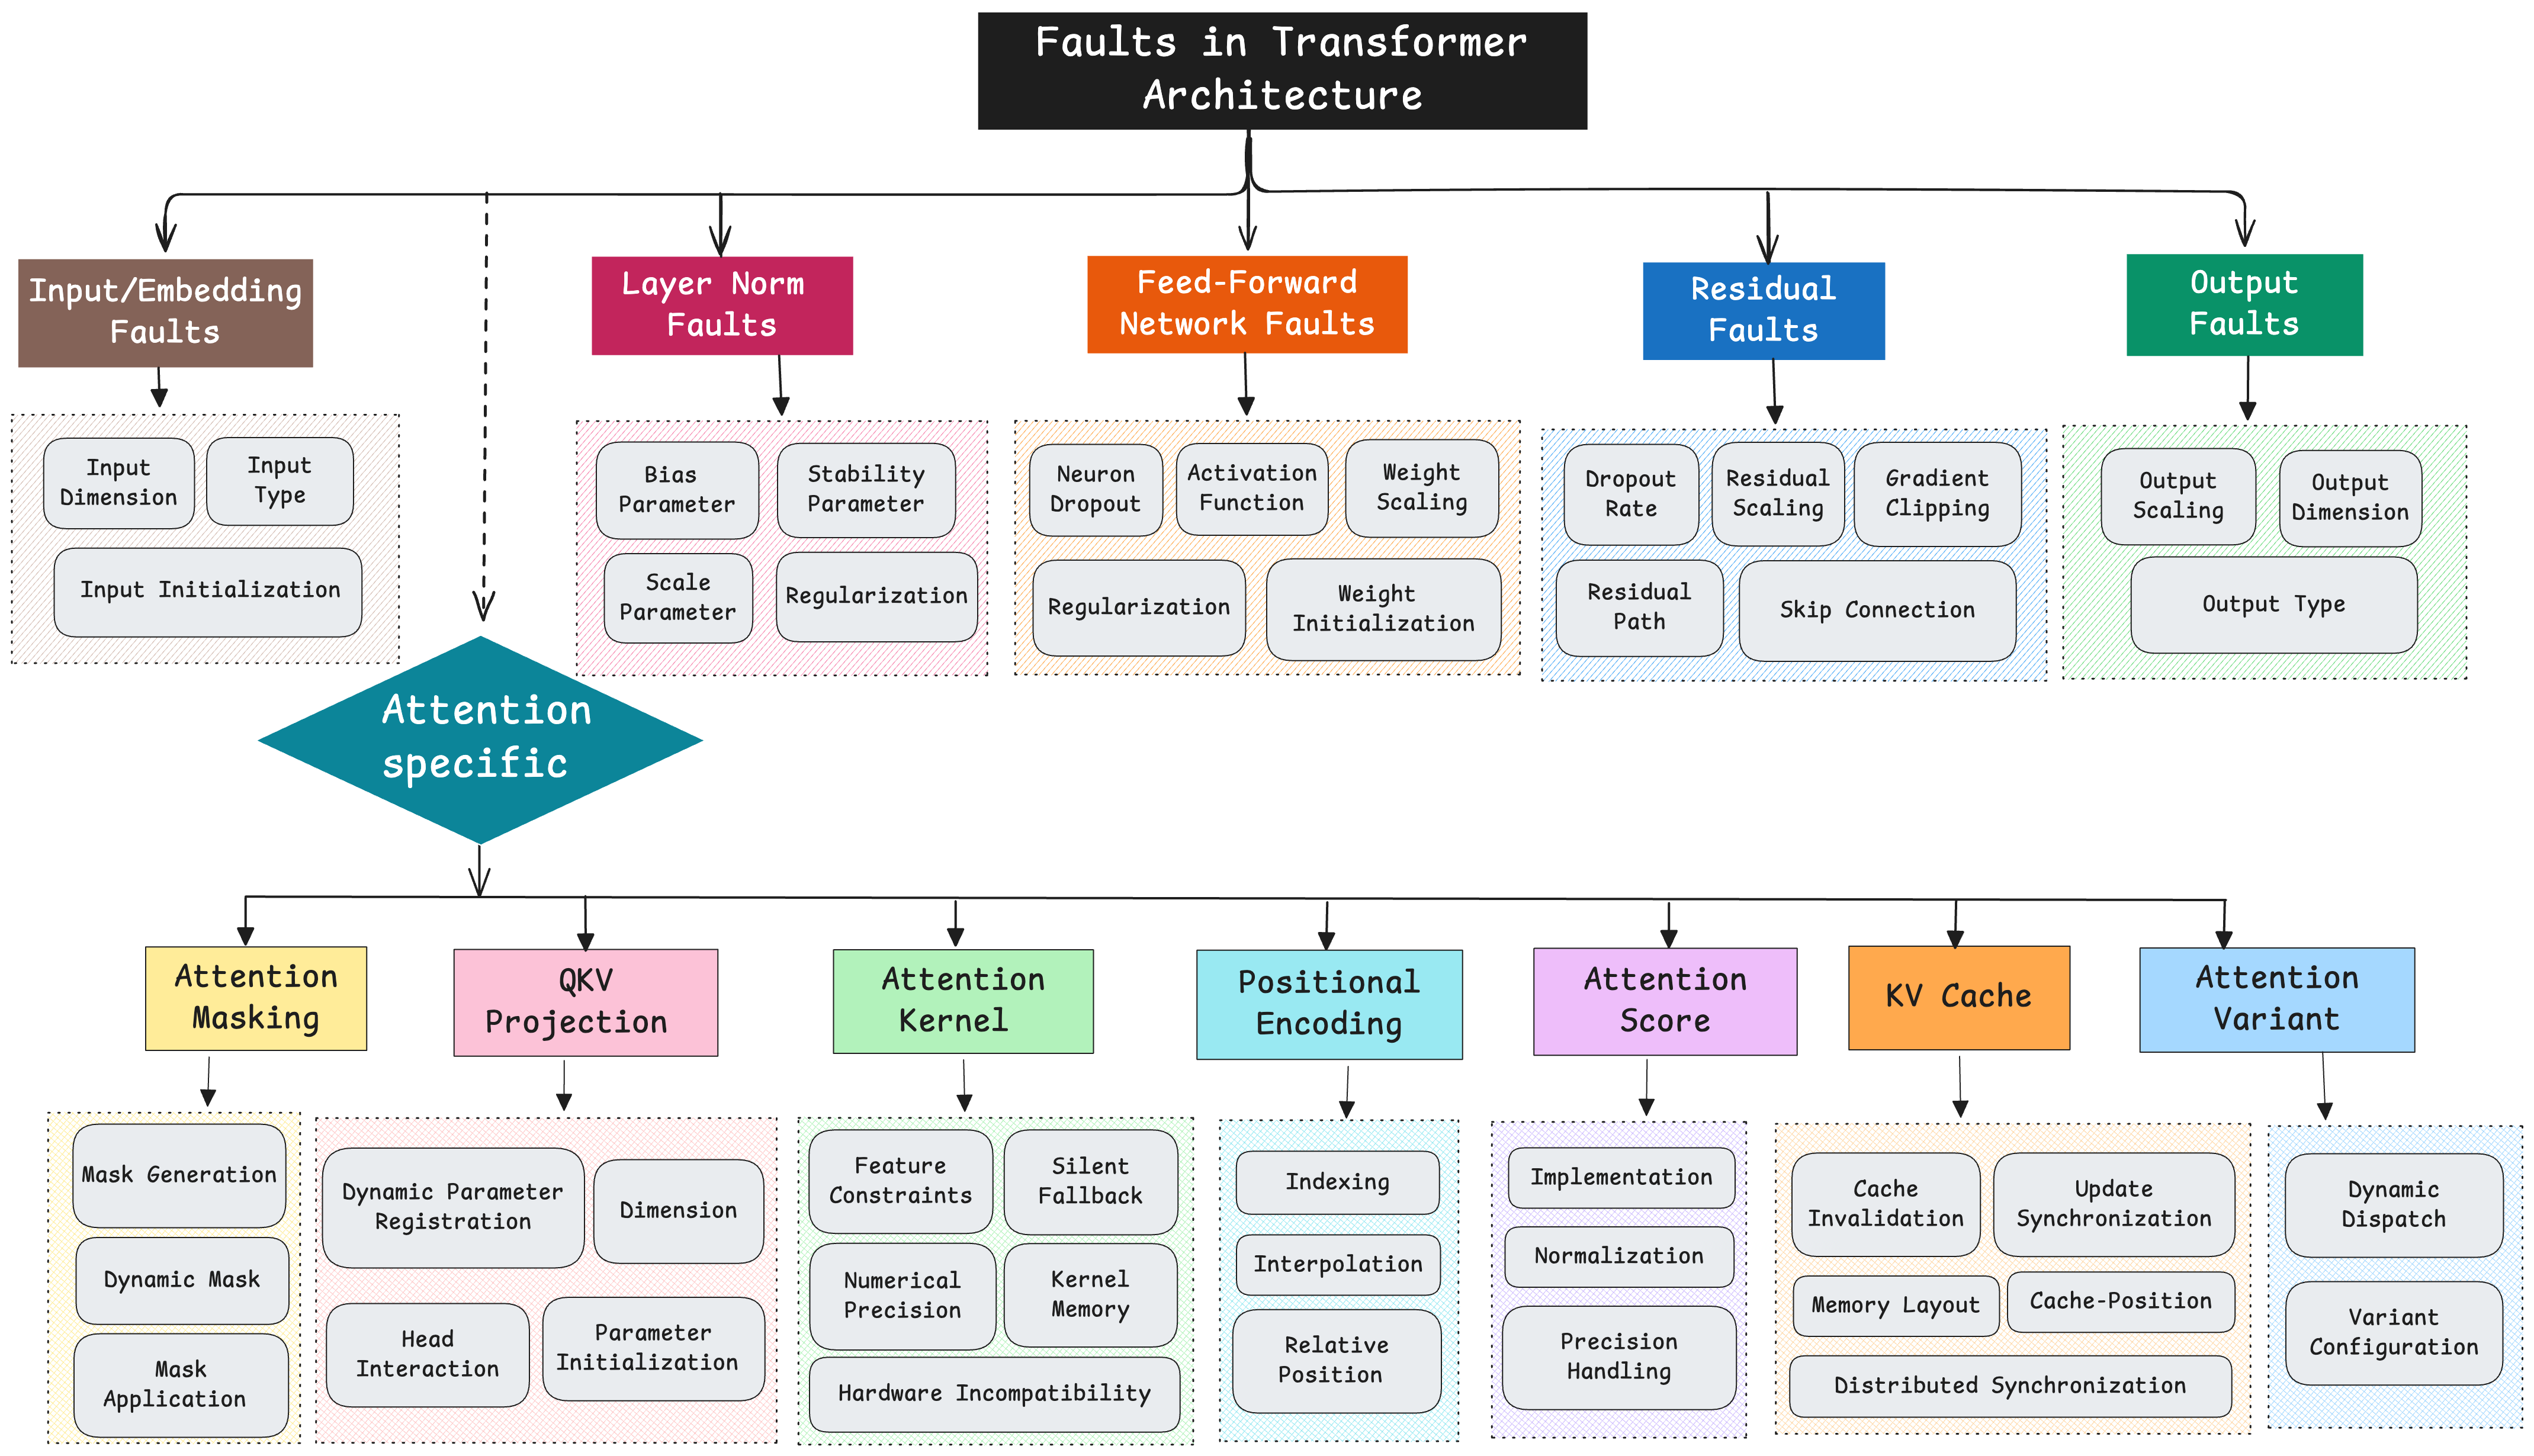
\includegraphics[width=\textwidth]{taxonomy-chapter-7-8.png}
\caption[Fault taxonomy defining the Level~2 and Level~3 label spaces.]{Complete fault taxonomy for transformer architectures. The seven attention-specific categories (bottom) and 25 root causes are from the attention fault taxonomy (Chapter~\ref{chapter_attention}). The five non-attention categories (top) and 20 root causes are from prior DNN fault taxonomies and DeepCrime.}
\label{fig:defaultpp-fault-taxonomy}
\end{figure}

The encoder and decoder subsets in Table~\ref{tab:data_accounting} are imbalanced. Encoder instances are 84.5\% faulty and decoder instances are 63.9\% faulty. For Levels~2 and~3, the 11--12 fault categories and their root causes also vary in support. Section~\ref{sec:defaultpp_experiment} describes the evaluation criteria and class-weighting strategy used to address this imbalance.

%------------------------------------------------------------------------------
\subsection{Fault Propagation Graph}
\label{sec:defaultpp_fpg}

The fault categories and root causes defined in Section~\ref{sec:defaultpp_dataset} identify \emph{where} a fault originates, but they do not describe how a fault in one component affects other components during forward computation or backward gradient flow. A stale QKV projection, for example, not only corrupts the projection output but also shifts downstream attention scores, attention weights, and the residual stream. To capture these inter-component dependencies, we define the Fault Propagation Graph (FPG), a directed graph derived from the transformer forward pass, backward pass, architectural configuration, and autoregressive execution. The FPG serves two purposes in DEFault++: it structures the feature representation by mapping feature groups to transformer components (Section~\ref{sec:defaultpp_features}), and it provides the adjacency matrix for message passing in the diagnostic model (Section~\ref{sec:defaultpp_message_passing}).

We distinguish seven dependency mechanisms. Mechanisms~1--3 describe local propagation relations in the forward computation, Mechanism~4 captures their repeated application across stacked layers, Mechanism~5 captures backward gradient-flow dependencies, Mechanism~6 captures architecture-wide interventions that affect multiple components simultaneously, and Mechanism~7 captures temporal dependencies introduced by decoder caching. The current FPG collapses these dependency types into unlabeled directed edges. The resulting graph is deterministic in construction since it reflects the fixed computational graph of the transformer architecture. Each edge encodes a structural dependency through which a perturbation can propagate. Whether a specific perturbation produces an observable downstream effect depends on its magnitude, on intervening nonlinear operations (detailed below), and on the parameter values learned during training. The FPG therefore models possible dependency pathways.

Existing works have used graph-based representations in DNN fault analysis for different purposes. NeuraLint~\cite{NeuraLint} models a deep-learning program as a typed meta-model graph and applies graph-transformation rules to detect structural faults before training. FL4Deep~\cite{fl4deep} constructs a knowledge graph from static and dynamic system information and uses reasoning together with learned link prediction to rank potential root causes. However, these graph representations do not model how a fault in one transformer component can propagate to other components through the forward computation or backward gradient flow. To address this gap, the FPG models fault propagation pathways within transformer architectures, with edges derived from dependencies in the transformer forward and backward pass.

We define the FPG $\mathcal{G} = (\mathcal{V}, \mathcal{E})$ where each node $v \in \mathcal{V}$ represents a transformer component. The component types are: embedding, positional encoding, QKV projection, score computation, attention masking, attention weights, attention output, residual connections, LayerNorm, FFN, and output head. Residual connections and LayerNorm appear independently for each sublayer (attention and FFN). Decoders additionally include a KV cache node. Each directed edge $(v_i, v_j) \in \mathcal{E}$ indicates that $v_j$ depends on $v_i$ under the chosen computational, execution, or architectural abstraction, so a perturbation at $v_i$ can reach $v_j$. An edge $(v_i, v_j)$ is included when a perturbation at $v_i$ can directly affect the output of $v_j$ through forward data flow, backward gradient flow, residual identity flow, autoregressive state reuse, or architecture-wide intervention under the chosen transformer abstraction. The FPG models only transformer components and their dependencies. Not all diagnostic feature groups are FPG nodes. Model-wide context groups and the cross-layer observation group participate in the group-level graph through self-loops only (Table~\ref{tab:fpg_mapping}).

By analyzing the transformer's forward and backward equations, we identify seven dependency mechanisms. Let $\delta x$ denote a perturbation to variable $x$.

\begin{enumerate}[nosep]
\item \textbf{M1: Forward sequential propagation.} If $B = f(A)$, then $\delta B = (\partial f / \partial A)\, \delta A$. Perturbation propagates along the data flow path: embedding $\to$ projections $\to$ scores $\to$ masking $\to$ weights $\to$ output $\to$ residual $\to$ LayerNorm $\to$ FFN $\to$ residual $\to$ output head.

\item \textbf{M2: Simultaneous propagation.} QKV projections feed both score computation (via $Q, K$) and attention output (via $V$) simultaneously. A single projection fault therefore perturbs scores and values at the same time. In decoders, $K$ and $V$ additionally enter the cache.

\item \textbf{M3: Residual bypass.} In $h = x + \text{MHA}(x)$, a perturbation $\delta x$ appears in $h$ with unit gain regardless of what the attention sublayer might do. Skip connections guarantee that faults cannot be absorbed by the sublayer they bypass.

\item \textbf{M4: Cross-layer propagation.} The residual stream propagates perturbations with at least unit gain per layer~\cite{roquet2024cross}. After $N$ layers, a fault in layer $\ell$ is present in all representations $\ell+1, \ldots, \ell+N$.

\item \textbf{M5: Backward pass propagation.} Any fault that changes the loss $\mathcal{L}$ changes $\partial \mathcal{L} / \partial \theta_i$ for every parameter $\theta_i$, affecting weight updates of every component during training.

\item \textbf{M6: Architecture-wide intervention.} Some fault types inherently affect multiple components at once. A variant fault (e.g., single-head instead of multi-head attention) simultaneously changes the attention computation pattern, parameter shapes, and kernel dispatch. Unlike Mechanisms~1--5, this is not a propagation relation but a structural co-affectation pattern in which a single architectural change alters multiple components at the same time.

\item \textbf{M7: Cache propagation across time steps} (decoder only). The KV cache stores $K$ and $V$ across generation steps. A cache fault affects the current token and all future tokens.
\end{enumerate}

Three nonlinear operations limit propagation at specific edges. Softmax maps perturbations into $[0,1]$ with a sum-to-one constraint, which reduces large-magnitude deviations. LayerNorm~\cite{ba2016layer} rescales outputs to zero mean and unit variance, which removes additive shifts. Activation functions (ReLU, GELU) suppress perturbations in their saturation regions and pass them in their linear regions. We annotate these limiting operations on the corresponding edges of the FPG.

The seven mechanisms fall into three classes (see Table~\ref{tab:fpg_derivation}). \emph{Propagation relations} (Mechanisms~1, 2, 3, 5, 7) describe how a perturbation at one component directly reaches another through forward data flow, residual identity, backward gradient flow, or autoregressive state reuse. \emph{Recursive composition} (Mechanism~4) is the repeated application of propagation relations~1 and~3 across stacked layers. \emph{Structural intervention} (Mechanism~6) is a co-affectation pattern in which a single architectural change simultaneously alters multiple components rather than propagating from one to another. The current FPG collapses all three classes into unlabeled directed edges. Relation-typed message passing that distinguishes these classes is a natural extension.

\begin{table}[!htbp]
\caption{Edge derivation for the Fault Propagation Graph. M3, M4, M5, and M6 entries represent dependency patterns that span multiple edges rather than individual directed connections.}
\label{tab:fpg_derivation}
\centering
\footnotesize
\renewcommand{\arraystretch}{1.0}
\begin{tabularx}{\textwidth}{@{} l l l c X @{}}
\toprule
\textbf{Source} & \textbf{Target} & \textbf{Mechanism Class} & \textbf{Scope} & \textbf{Details} \\
\midrule
Embedding & QKV Projection & Forward prop.\ (M1) & Enc/Dec & $Q,K,V = W_{Q,K,V}\, E[x]$ \\
Positional & QKV Projection & Forward prop.\ (M1) & Enc/Dec & Position added to embedding before projection \\
QKV Proj.\ & Score Computation & Simultaneous (M2) & Enc/Dec & $S = QK^\top\!/\sqrt{d_k}$; $Q,K$ from projection \\
QKV Proj.\ & Attn.\ Output & Simultaneous (M2) & Enc/Dec & $\text{Attn} = \text{softmax}(S)\,V$; $V$ from projection \\
QKV Proj.\ & KV Cache & Simultaneous (M2) & Dec & $K,V$ stored in cache at each step \\
Score Comp.\ & Attn.\ Masking & Forward prop.\ (M1) & Enc/Dec & $S' = S + M$ \\
Attn.\ Masking & Attn.\ Weights & Forward prop.\ (M1) & Enc/Dec & $\alpha = \text{softmax}(S')$ \\
Attn.\ Weights & Attn.\ Output & Forward prop.\ (M1) & Enc/Dec & $\text{Attn} = \alpha\, V$ \\
Attn.\ Output & Residual (attn) & Forward prop.\ (M1) & Enc/Dec & $h = x + \text{Attn}(x)$ \\
Residual input & Residual (attn) & Residual bypass (M3) & Enc/Dec & Skip connection: $\delta x$ passes with unit gain \\
Residual (attn) & LayerNorm (attn) & Forward prop.\ (M1) & Enc/Dec & $\hat{x} = \text{LN}(h)$ \\
LayerNorm (attn) & FFN & Forward prop.\ (M1) & Enc/Dec & FFN input is post-norm representation \\
FFN & Residual (FFN) & Forward prop.\ (M1) & Enc/Dec & $h' = h + \text{FFN}(\hat{x})$ \\
Residual input & Residual (FFN) & Residual bypass (M3) & Enc/Dec & Skip connection: $\delta h$ passes with unit gain \\
Residual (FFN) & LayerNorm (FFN) & Forward prop.\ (M1) & Enc/Dec & $\hat{h}' = \text{LN}(h')$ \\
LayerNorm (FFN) & Output Head & Forward prop.\ (M1) & Enc/Dec & Final representation enters output head \\
Layer $\ell$ residual & Layer $\ell{+}1$ & Cross-layer (M4) & Enc/Dec & Repeated M1+M3 across stacked layers \\
All components & All components & Backward prop.\ (M5) & Enc/Dec & $\partial\mathcal{L}/\partial\theta_i$ couples all parameters \\
KV Cache & Attn.\ Weights & Cache-time (M7) & Dec & Cached $K,V$ affect future-step attention \\
Variant config.\ & Multiple components & Intervention (M6) & Enc/Dec & Architectural change alters multiple components \\
\bottomrule
\end{tabularx}
\end{table}

\begin{figure}[!htbp]
\centering
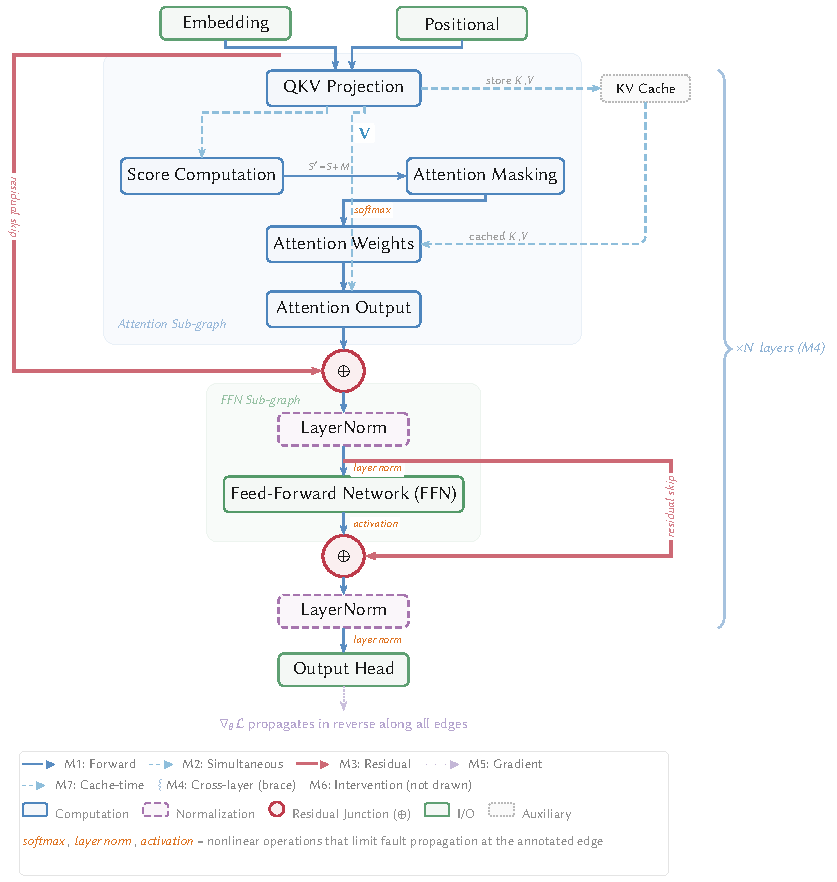
\includegraphics[width=0.85\linewidth]{fig_fpg.pdf}
\caption{The Fault Propagation Graph (FPG) for transformer architectures. The cross-layer loopback represents M4. The dashed return from KV Cache to Attention Weights represents M7 (decoder only). M6 is omitted because it affects multiple components simultaneously.}
\label{fig:defaultpp_fpg}
\end{figure}

For use in the diagnostic model, we collapse the component-level FPG to a group-level adjacency matrix. Each transformer component maps to the feature group that instruments it, as shown in Table~\ref{tab:fpg_mapping}. A group-level edge exists if any component in the source group has a propagation edge to any component in the target group. Components that map to the same group (e.g., attention masking, attention weights, and attention output all map to the Attention group) are merged. Structural groups receive FPG-derived neighbor edges. The cross-layer observation group (Representation drift) and model-wide context groups (Training dynamics, Validation performance) participate through self-loops only: they undergo the same learned transformation as structural groups but do not receive information from neighboring groups. Groups that map to multiple components inherit all edges of their constituent components. Figure~\ref{fig:defaultpp_adjacency} shows the group-level adjacency matrix $\hat{\mathbf{A}}$ for the decoder diagnostic model ($G = 13$). The near-diagonal sparsity reflects the sequential data flow through the transformer block, while the off-diagonal entries (e.g., QKV$\to$Cache, Cache$\to$Attention, FFN$\to$Residual) capture the feedback and branching paths that the FPG encodes. Non-structural groups (Representation drift, Training dynamics, Validation performance) appear as isolated self-loops in the lower-right block.

\begin{figure}[!htbp]
\centering
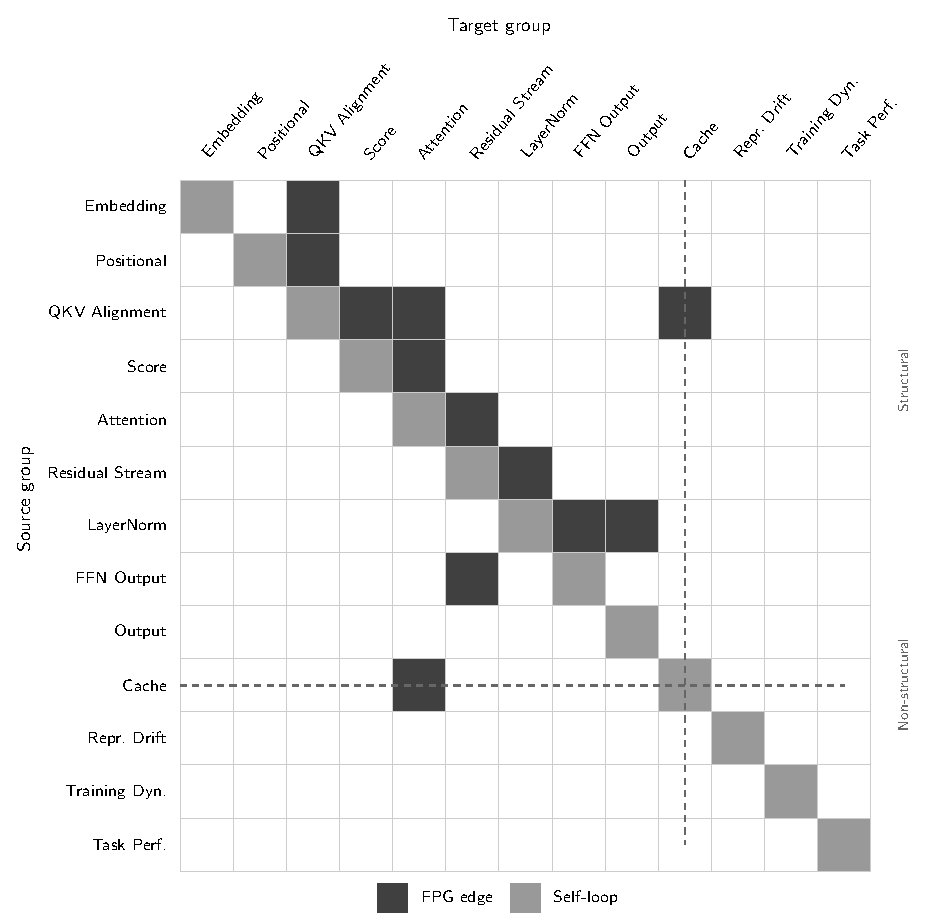
\includegraphics[width=0.72\linewidth]{fig_adjacency_matrix.pdf}
\caption{Group-level adjacency matrix $\hat{\mathbf{A}}$ for the decoder diagnostic model.}
\label{fig:defaultpp_adjacency}
\end{figure}

\begin{table}[!htbp]
\caption{Feature-group roles and message passing in DEFault++. Structural groups use FPG-derived edges. Cross-layer observation and model-wide context groups use self-loops only.}
\label{tab:fpg_mapping}
\centering
\footnotesize
\renewcommand{\arraystretch}{1.0}
\begin{tabular}{@{} l l l l @{}}
\toprule
\textbf{Feature Group} & \textbf{Role} & \textbf{Scope} & \textbf{Message Passing} \\
\midrule
Attention & Structural & Attention masking, weights, output & FPG edges \\
Score & Structural & Score computation & FPG edges \\
FFN output & Structural & FFN & FPG edges \\
LayerNorm & Structural & LayerNorm & FPG edges \\
Residual stream & Structural & Residual connections & FPG edges \\
QKV alignment & Structural & QKV projection & FPG edges \\
Embedding & Structural & Embedding & FPG edges \\
Positional & Structural & Positional encoding & FPG edges \\
Output & Structural & Output head & FPG edges \\
Cache (dec.) & Structural & KV cache & FPG edges \\
\midrule
Representation drift & Cross-layer observation & Inter-layer residual path & Self-loop only \\
\midrule
Training dyn. & Model-wide context & Model-wide optimization & Self-loop only \\
Validation perf. & Model-wide context & Model-wide output quality & Self-loop only \\
\bottomrule
\end{tabular}
\end{table}

%------------------------------------------------------------------------------
\subsection{Feature Representation}
\label{sec:defaultpp_features}

The Fault Propagation Graph defines which transformer components can affect each other, but the diagnostic model requires quantitative measurements of those components during training. Generic DNN fault features such as loss trajectories, gradient statistics, and activation counts do not distinguish transformer fault categories~\cite{frankenformer}. Corrupted QKV projections, missing causal masks, and misconfigured positional encodings leave end-task metrics undisturbed while producing characteristic patterns in attention-level and component-level measurements. We therefore define a transformer-specific feature space that targets attention distributions, projection alignments, and residual-stream behavior (see Figure~\ref{fig:feature_technique}). Table~\ref{tab:defaultpp_features} lists the feature groups, their metric types, and the collection branch through which each group enters the feature-construction process.

\begin{table}[!htbp]
\caption{Feature groups, metric types, and dimensionality derivation in DEFault++.}
\label{tab:defaultpp_features}
\centering
\footnotesize
\renewcommand{\arraystretch}{1.05}
\begin{tabularx}{\linewidth}{@{} p{1.7cm} X c @{}}
\toprule
\textbf{Feature Group} & \textbf{Metric Types} & $\mathbf{n_g}$ \\
\midrule

\multicolumn{3}{c}{\textit{Layer-internal metrics ($C_{int}$, collected at each training step, per layer)}} \\[2pt]

Attention & Attention entropy, padding attention mass, inter-head cosine similarity, head utilization, attention rank, cross-example leakage, future attention mass (decoder only) & 6/7\textsuperscript{a} \\[2pt]

Score & Pre-softmax score & 1 \\[2pt]

FFN output & FFN output norm & 1 \\[2pt]

LayerNorm & Scale parameter norm, post-norm distribution & 2 \\[2pt]

Residual stream & Residual cosine similarity & 1 \\[2pt]

Repr.\ drift & CKA layer similarity & 1 \\[2pt]

QKV alignment & Q--K sim., Q--V sim., K--V sim. & 3 \\[2pt]

\midrule
\multicolumn{3}{c}{\textit{Gradient metrics ($C_{opt}$, collected at each training step)}} \\[2pt]

Optimization & Component-level and global gradient features (gradient norm, update ratio, update activity) & 21 \\[2pt]

\midrule
\multicolumn{3}{c}{\textit{Behavioral metrics ($C_{train}$, collected at each training step)}} \\[2pt]

Embedding & Embedding norm, token-level variance & 2 \\[2pt]

Positional & Positional sensitivity & 1 \\[2pt]

Training dyn. & Loss trajectory, gradient noise scale, step time, peak memory allocation & 4 \\[2pt]

Output & Prediction confidence, output entropy, margin statistics & 3 \\[2pt]

Cache & Cache hidden similarity, cache distribution divergence & 2 \\[2pt]

\midrule
\multicolumn{3}{c}{\textit{Validation metrics ($C_{eval}$, collected at epoch end or validation checkpoints)}} \\[2pt]

Validation perf. & Task accuracy / perplexity, calibration error & 2 \\

\midrule

\multicolumn{3}{@{}p{\linewidth}@{}}{\textsuperscript{a}6 for encoders, 7 for decoders (future attention mass applies only to decoders).} \\[2pt]

\multicolumn{3}{@{}p{\linewidth}@{}}{\textbf{Branch Total (see Figure~\ref{fig:feature_technique}):}
$C_{int}=15$ (encoder) / $16$ (decoder), $C_{opt}=21$, $C_{train}=10$ (encoder) / $12$ (decoder), $C_{eval}=2$.} \\[2pt]

\multicolumn{3}{@{}p{\linewidth}@{}}{\textbf{Aggregation factors:}
$A_{\ell}=5$ for layer aggregation
(early $\mu$, early $\sigma$, mid $\mu$, mid $\sigma$, final-layer value),
$A_e=3$ for epoch summary (epoch $\mu$, epoch $\sigma$, burst),
and $A_p=5$ for training-phase summary (early $\mu$, mid $\mu$, final $\mu$, slope, final value).} \\[2pt]

\multicolumn{3}{@{}p{\linewidth}@{}}{\textbf{Dimensionality:}
$d_{\text{step}} = A_{\ell}C_{int}+C_{opt}+C_{train}$,
$d_{\text{epoch}} = A_e d_{\text{step}} + C_{eval}$,
$d_{\text{final}} = A_p d_{\text{epoch}}$.} \\[2pt]

\multicolumn{3}{@{}p{\linewidth}@{}}{\textbf{Closed form:}
$d_{\text{final}} = A_p\!\left(A_e\!\left(A_{\ell}C_{int}+C_{opt}+C_{train}\right)+C_{eval}\right)$.} \\[2pt]

\multicolumn{3}{@{}p{\linewidth}@{}}{\textbf{Final feature-vector size:}
encoder $= 5\!\left(3\!\left(5\!\cdot\!15+21+10\right)+2\right)=5\!\left(3\!\cdot\!106+2\right)=1600$,
decoder $= 5\!\left(3\!\left(5\!\cdot\!16+21+12\right)+2\right)=5\!\left(3\!\cdot\!113+2\right)=1705$.} \\

\bottomrule
\end{tabularx}
\end{table}


\vspace{0.5em}
\noindent\textbf{\textsc{A. Layer-internal metrics}} ($C_{int}$, collected per layer at each training step).

\paragraph{A1-Attention.} We measure seven properties of the post-softmax attention distribution at each sampled layer (six for encoders, seven for decoders). \emph{Attention entropy} ($H_{\text{attn}}$, Equation~\ref{eq:entropy}) computes the Shannon entropy of the attention distribution, averaged across heads and query positions~\cite{voita2019analyzing}. Low entropy indicates that a head concentrates on a single position. High entropy indicates a near-uniform distribution. \emph{Padding attention mass} ($\mathrm{PadMass}$, Equation~\ref{eq:padmass}) computes the fraction of attention directed at padding tokens. Non-zero padding mass indicates a masking fault. \emph{Inter-head cosine similarity} ($\mathrm{HeadSim}$, Equation~\ref{eq:headsim}) computes pairwise cosine similarity $\text{sim}(\mathbf{a}_i, \mathbf{a}_j) = \frac{\mathbf{a}_i \cdot \mathbf{a}_j}{\|\mathbf{a}_i\|\,\|\mathbf{a}_j\|}$ between the flattened attention patterns of heads $i$ and $j$ within each layer. High pairwise similarity indicates redundant heads. \emph{Head utilization} is the fraction of heads whose attention entropy exceeds a minimum threshold, indicating the head attends to more than one position. Variant faults that reduce the effective head count lower this fraction~\cite{voita2019analyzing,clark2019does}. \emph{Attention rank} quantifies the effective dimensionality of each head's attention weight matrix using the exponential of the Shannon entropy of the normalized singular value distribution~\cite{roy2007effective}, as defined in Chapter~\ref{chapter_frankenformer} (Equation~\ref{eq:effrank}). A rank near~1 indicates the head attends to a single position; a rank near~$n$ indicates near-uniform attention. Variant faults that reduce multi-head capacity reduce the metric, while faults that collapse heads to uniform distributions increase it. \emph{Cross-example leakage} measures the total attention weight flowing between unrelated examples in the same batch, averaged over heads and layers~\cite{vaswani2017attention,dao2022flashattention}. Under correct masking, this quantity is zero. Non-zero values indicate that the attention mechanism attends across example boundaries, which is a direct indicator of masking faults. \emph{Future attention mass} (decoder only) measures the total attention weight assigned from each query position to future key positions, averaged over heads and layers (Equation~\ref{eq:futuremass})~\cite{vaswani2017attention}. Under correct causal masking, this quantity is near zero. Causal-mask violations increase it systematically. This metric applies only to decoder architectures, where the causal constraint restricts each token to attending only to preceding positions.

\paragraph{A2-Score.} We record the raw attention logits before the softmax operation~\cite{vaswani2017attention}:
\begin{equation}
s = Q K^\top / \sqrt{d_k}.
\label{eq:score_stats}
\end{equation}
At each layer, we reduce the full query-key score matrix to a single scalar by computing its mean across all positions~\cite{dong2021attention}. This within-layer reduction precedes the cross-layer aggregation ($A_\ell$) described above. High score variance across layers indicates that attention sharpness differs substantially between early and late layers, which can result from softmax saturation and reduced gradient flow~\cite{dong2021attention,zhai2023stabilizing}. Pre-softmax scores are sensitive to Score and Positional faults because both fault types directly alter this computation.

\paragraph{A3-FFN output.} We record the $\ell_2$ norm of the feed-forward sublayer outputs at each layer, computed as $\|\text{FFN}(x)\|_2$ per token and averaged across the batch. Abnormally large norms indicate instability in the FFN transformation. Near-zero norms indicate that the FFN sublayer contributes little to the residual stream, which can occur when activation functions suppress most dimensions.

\paragraph{A4-LayerNorm.} We record two properties of layer normalization~\cite{ba2016layer} at each layer. \emph{Scale parameter norm} is the Frobenius norm $\|\gamma\|_F$ of the learned scale vector. \emph{Post-norm distribution} captures the moments of the normalized output:
\begin{equation}
\hat{x} = \gamma \odot \frac{x - \mu}{\sigma + \epsilon} + \beta.
\label{eq:layernorm}
\end{equation}
A LayerNorm fault disrupts the rescaling to zero mean and unit variance, producing abnormal post-norm moments or $\gamma$ magnitudes that differ from values observed in clean training runs.

\paragraph{A5-Residual stream.} We compute the cosine similarity between the input and output of each residual sublayer:
\begin{equation}
\text{res\_sim}_\ell = \frac{x_\ell \cdot h_\ell}{\|x_\ell\|\,\|h_\ell\|}
\label{eq:residual_sim}
\end{equation}
where $x_\ell$ is the sublayer input and $h_\ell = x_\ell + f(x_\ell)$ is the residual output at layer $\ell$. In a correctly functioning transformer, the skip connection preserves the input direction while the sublayer $f$ adds a bounded perturbation, so cosine similarity remains close to 1.0. A Residual fault that corrupts the skip-connection path reduces this similarity. This metric measures the effect of a fault \emph{within} a single sublayer (input vs.\ output of the same residual block).

\paragraph{A6-Representation drift.} We compute Centered Kernel Alignment (CKA)~\cite{kornblith2019similarity} between consecutive layer representations:
\begin{equation}
\text{CKA}(H_\ell, H_{\ell+1}) = \frac{\|H_{\ell+1}^\top H_\ell\|_F^2}{\|H_\ell^\top H_\ell\|_F \;\|H_{\ell+1}^\top H_{\ell+1}\|_F}
\label{eq:cka}
\end{equation}
where $H_\ell \in \mathbb{R}^{n \times d}$ is the centered representation matrix at layer $\ell$. CKA measures similarity independent of rotation and isotropic scaling. A fault that propagates across multiple layers causes decreasing CKA between adjacent layers. We use CKA rather than direct cosine similarity because CKA is invariant to orthogonal transformations of the representation space. Unlike the Residual stream metric, which measures the effect of a single sublayer on its own input, CKA measures cumulative representational change \emph{between} consecutive layers and therefore captures faults that propagate beyond the originating sublayer.

\paragraph{A7-QKV alignment.} We compute pairwise cosine similarity between the query, key, and value projection outputs at each sampled layer:
\begin{equation}
\text{sim}(Q, K) = \frac{Q \cdot K}{\|Q\|\,\|K\|}, \quad \text{sim}(Q, V) = \frac{Q \cdot V}{\|Q\|\,\|V\|}, \quad \text{sim}(K, V) = \frac{K \cdot V}{\|K\|\,\|V\|}
\label{eq:qkv_alignment}
\end{equation}
where $Q = W_Q x$, $K = W_K x$, and $V = W_V x$ are the projection outputs for input $x$~\cite{vaswani2017attention}. A fault that corrupts one projection weight matrix shifts its output direction relative to the other two, producing a measurable drop in pairwise similarity.

\vspace{0.5em}
\noindent\textbf{\textsc{B. Gradient metrics}} ($C_{opt}$, collected per component at each training step).

For each parameterized component (e.g., Attention, QKV, FFN, LayerNorm, Embedding), we compute three gradient-level measurements inspired by prior DNN fault detection work~\cite{default,deepfd}. \emph{Gradient norm} computes the $\ell_2$ norm of the gradient vector for all parameters belonging to that component:
\begin{equation}
g_c = \sqrt{\sum_{\theta \in \Theta_c} \|\nabla_\theta \mathcal{L}\|^2}
\label{eq:component_grad_norm}
\end{equation}
where $\Theta_c$ is the parameter set of component $c$. \emph{Update ratio} measures the relative magnitude of weight change between consecutive training steps:
\begin{equation}
u_c = \frac{\|W_c^{(t)} - W_c^{(t-1)}\|_F}{\|W_c^{(t-1)}\|_F + \epsilon}
\label{eq:component_update_ratio}
\end{equation}
where $W_c^{(t)}$ is the weight matrix of component $c$ at step $t$. \emph{Update activity} is a binary flag indicating whether the gradient norm exceeds a minimum threshold ($g_c > 10^{-6}$), which identifies components that have stopped learning. These 15 component-level measurements (three per component) together with six global gradient statistics form the $C_{opt}=21$ gradient metrics in Table~\ref{tab:defaultpp_features}. The Output group uses behavioral metrics only and does not add a sixth component-routed gradient set.

\vspace{0.5em}
\noindent\textbf{\textsc{C. Behavioral metrics}} ($C_{train}$, collected at each training step).

\paragraph{C1-Embedding.} We record two properties of the input embedding vectors. \emph{Embedding norm} is the mean $\ell_2$ norm $\frac{1}{n}\sum_{i=1}^{n}\|e_i\|_2$ across all $n$ input tokens, where $e_i = E[x_i]$ is the embedding of token $x_i$. \emph{Token-level variance} is $\text{Var}(\{e_1, \ldots, e_n\})$ computed across the hidden dimension. An Embedding fault that corrupts the embedding matrix $E$ produces abnormal norms or collapses the variance across tokens. We compute both metrics on the first hidden state before the first transformer block.

\paragraph{C2-Positional.} We measure positional sensitivity from the model's response to a fixed non-zero shift in position indices on a held-out batch, using the same perturbation protocol as Chapter~\ref{chapter_frankenformer}. In all experiments, we set $\Delta = 1$. Let $P_{\max}$ denote the model's maximum supported position index, and let $\mathcal{I}(X)$ be the set of valid non-padding token positions in batch $X$ such that $i+\Delta < P_{\max}$. For each $i \in \mathcal{I}(X)$, we compare the hidden state at position $i$ under the original indices with the hidden state at the same token position under the shifted indices. We define positional sensitivity as
\begin{equation}
S_{\text{pos}}(X) =
\frac{1}{L\,|\mathcal{I}(X)|}
\sum_{\ell=1}^{L}
\sum_{i \in \mathcal{I}(X)}
\left\|
h_{\ell,i}(X) - h_{\ell,i}^{(\Delta)}(X)
\right\|_2
\label{eq:positional_sensitivity}
\end{equation}
where $L$ is the number of instrumented layers. Tokens that would exceed the valid index range after shifting are excluded from the average; we do not clip, wrap, or reuse position indices. Larger values indicate stronger dependence of the model's representations on positional information. Positional faults that omit, misalign, or truncate positional encoding shift this quantity away from the clean baseline.

\paragraph{C3-Training dynamics.} We record four optimization-level and infrastructure-level metrics at each training step. \emph{Loss trajectory} is the scalar training loss per step. \emph{Gradient noise scale} measures the ratio of gradient variance to the squared gradient norm~\cite{mccandlish2018empirical}:
\begin{equation}
\text{GNS} = \frac{\text{Var}(\|\nabla \mathcal{L}\|)}{\mathbb{E}[\|\nabla \mathcal{L}\|]^2}
\label{eq:gns}
\end{equation}
computed over a rolling window of 20 training steps. High gradient noise scale indicates that individual batches produce inconsistent gradient directions. \emph{Step time} is the wall-clock duration of each training step. Sudden increases in step time can indicate memory pressure or scheduling faults. \emph{Peak memory allocation} records the peak GPU memory reported by the CUDA allocator during each training step~\cite{nvidia2021dlprof,chakrabarti2012cuda}. A forced fallback to a non-optimized kernel or an unintended data-layout change can increase peak memory without raising an explicit error~\cite{dao2022flashattention}. We include peak memory alongside step time because both are infrastructure-level measurements that detect kernel and scheduling faults.

\paragraph{C4-Output.} We record three properties of the output head at each training step. \emph{Prediction confidence} computes the mean maximum softmax probability $\frac{1}{N}\sum_{i=1}^{N} \max_c p_c^{(i)}$ across all samples in the batch. \emph{Output entropy} computes the mean Shannon entropy of the output distribution $-\frac{1}{N}\sum_{i=1}^{N}\sum_c p_c^{(i)} \log p_c^{(i)}$. \emph{Margin statistics} measure the gap between the correct-class logit and the strongest competing logit. For encoder classification tasks, we compute these metrics over the classification logits per batch sample. For decoder language modeling tasks, we average over non-padding tokens within each sequence, where margin measures the gap between the logit of the true next token and the highest competing logit. Low confidence, high entropy, or negative margins indicate that the output head does not produce well-separated predictions, which can result from faults in upstream components or from direct output-projection faults. These step-level per-batch measurements differ from the validation metrics (below), which aggregate accuracy and calibration at the epoch level.

\paragraph{C5-Cache (decoder only).} We measure two properties of the key-value cache used during autoregressive generation. \emph{Cache hidden similarity} computes the cosine similarity $\text{sim}(K_{\text{cached}}, K_{\text{recomputed}})$ between cached and recomputed key states at each generation step. High similarity indicates a consistent cache. Low similarity indicates stale or corrupted cached states. \emph{Cache distribution divergence} computes the KL divergence:
\begin{equation}
D_{\text{KL}}(P_{\text{cache}} \| P_{\text{fresh}}) = \sum_v P_{\text{cache}}(v) \log \frac{P_{\text{cache}}(v)}{P_{\text{fresh}}(v)}
\label{eq:cache_kl}
\end{equation}
between the next-token distribution produced using the cache ($P_{\text{cache}}$) and the distribution produced by fresh computation ($P_{\text{fresh}}$). Non-zero divergence indicates that cached states produce different predictions, which is a direct indicator of KV Cache faults.

\vspace{0.5em}
\noindent\textbf{\textsc{D. Validation metrics}} ($C_{eval}$, collected at epoch end or validation checkpoints).

We record two measurements at epoch end or at scheduled validation checkpoints. \emph{Task accuracy} is classification accuracy for encoder tasks and perplexity for decoder language modeling tasks. \emph{Calibration error} is the expected calibration error~\cite{guo2017calibration}:
\begin{equation}
\text{ECE} = \sum_{b=1}^{B} \frac{|b|}{N} \,\big|\text{acc}(b) - \text{conf}(b)\big|
\label{eq:defaultpp_ece}
\end{equation}
where $B$ is the number of confidence bins. Faults that degrade downstream performance produce abnormal values in these metrics. Faults that shift internal behavior without affecting validation performance (task-invisible faults) produce normal values in this group but abnormal values in other groups. Since these metrics are computed at epoch boundaries rather than at each training step, they enter the feature-construction process after the epoch-level summary stage (Table~\ref{tab:defaultpp_features}).

\begin{figure}[!htbp]
\centering
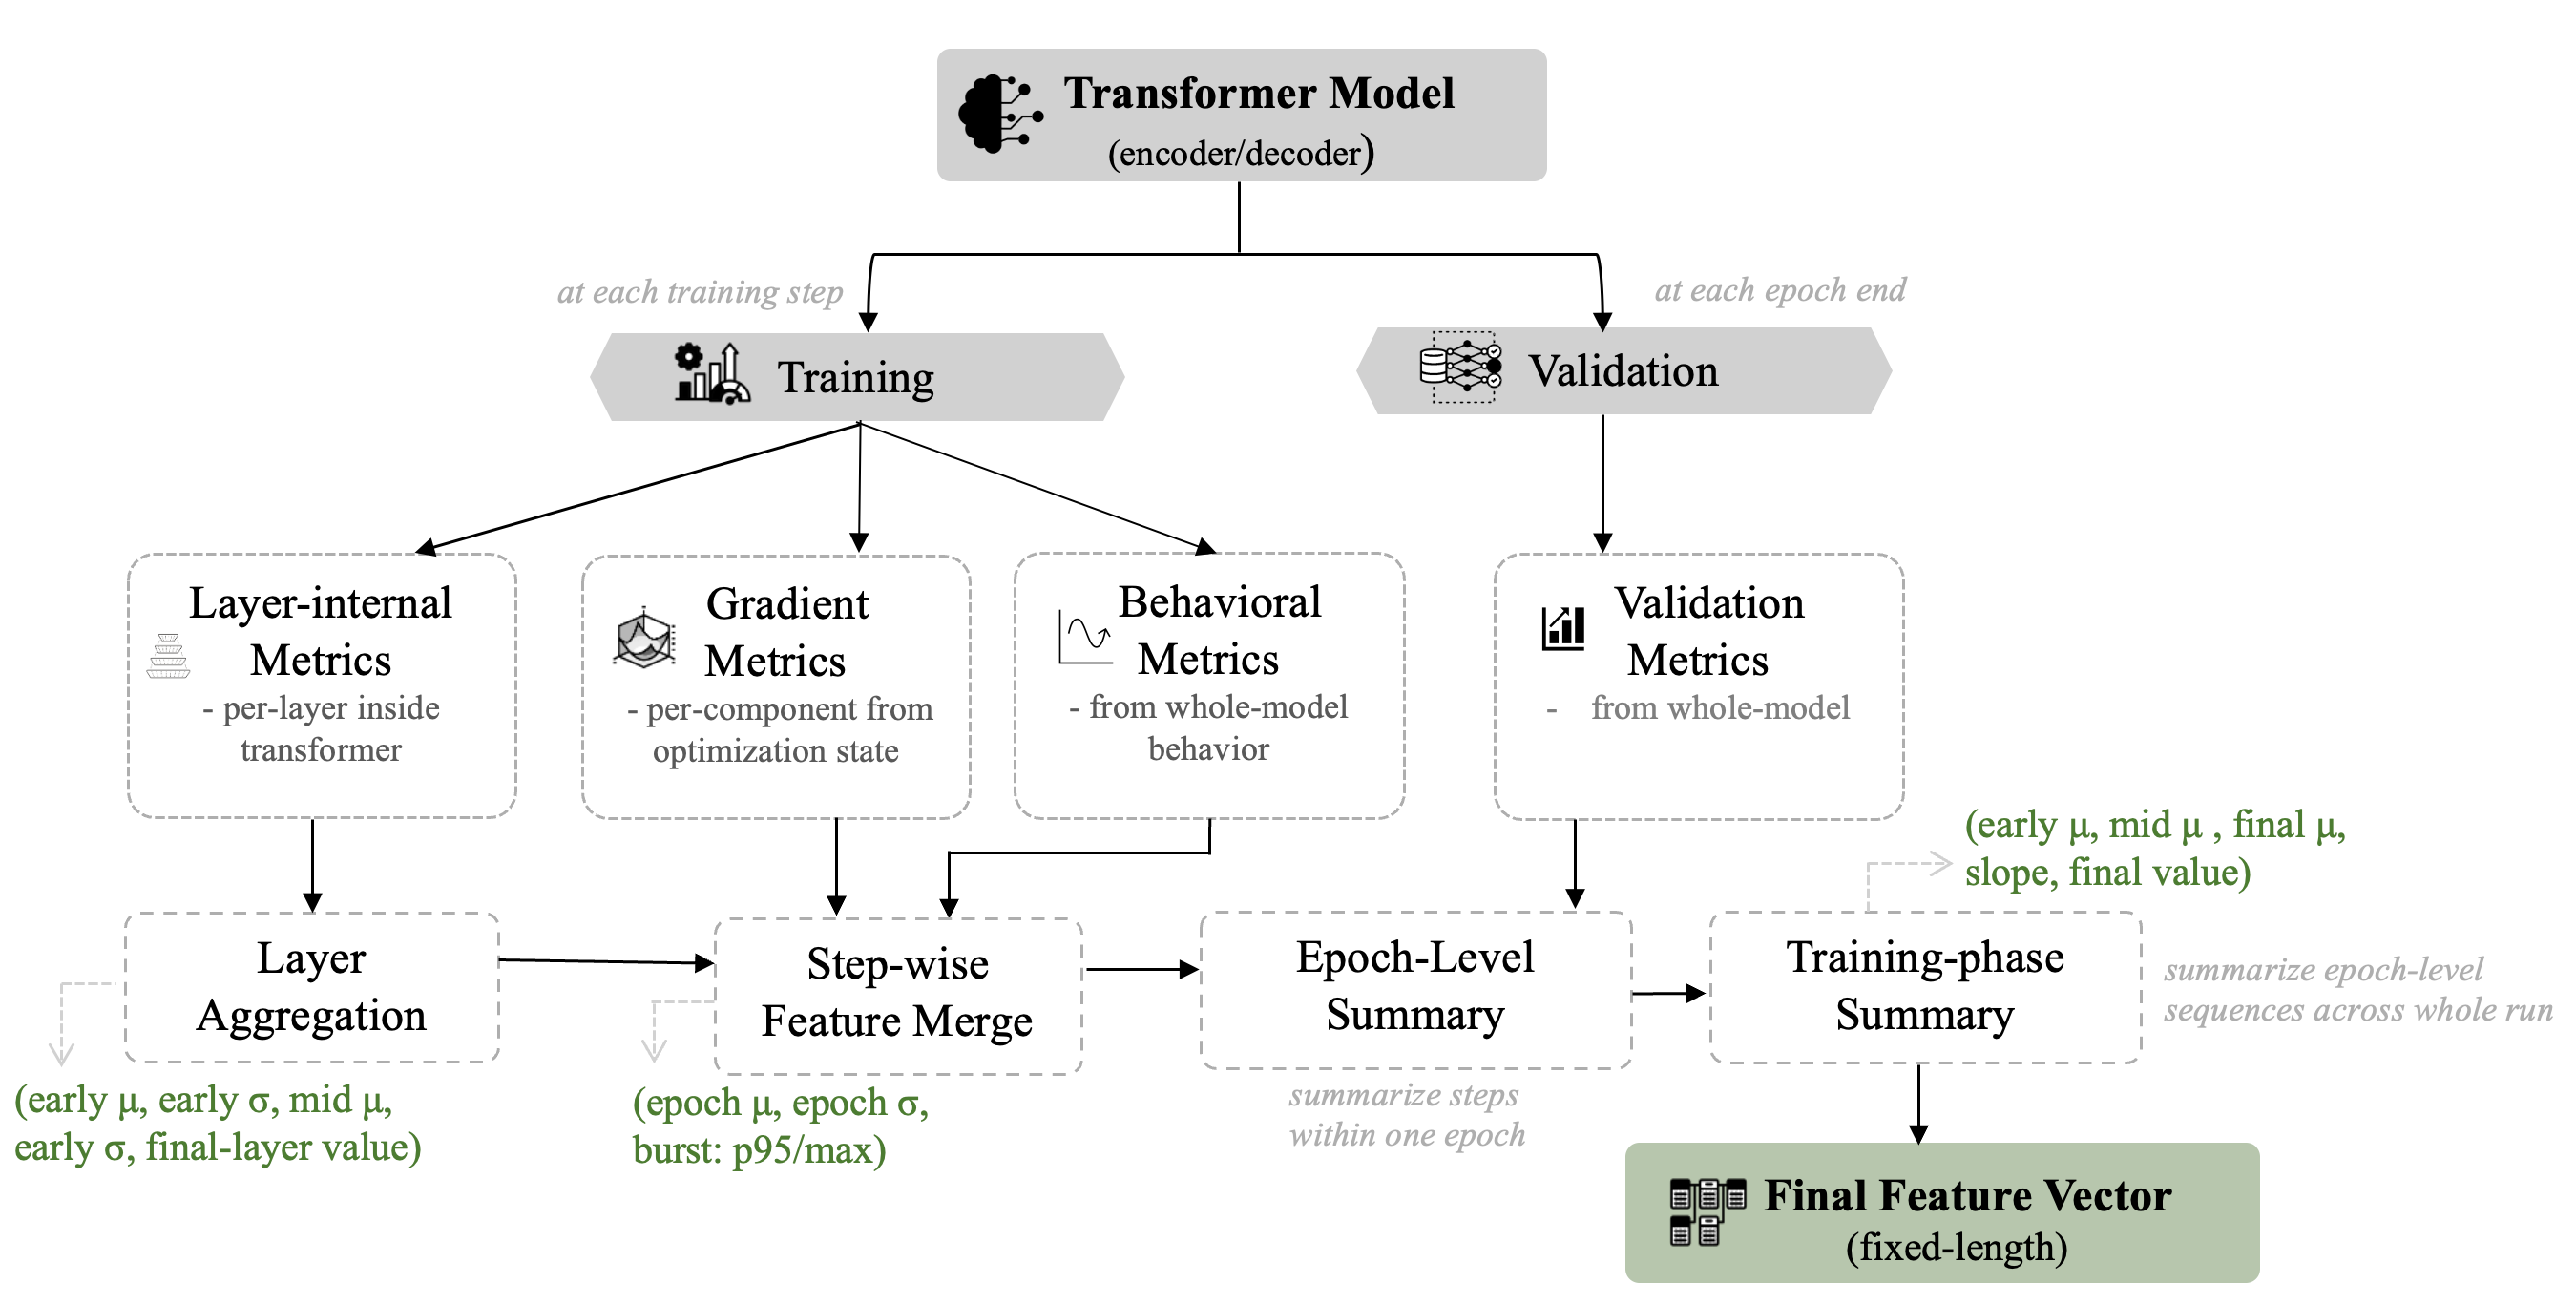
\includegraphics[width=0.98\linewidth]{fig_feature.png}
\caption{Feature-construction technique in DEFault++, from metric collection through aggregation to the final fixed-length feature vector.}
\label{fig:feature_technique}
\end{figure}

\subsubsection{Aggregation \& Feature Vector Construction}
\label{sec:defaultpp_aggregation}

We classify each metric into one of four collection branches based on its granularity (see Figure~\ref{fig:feature_technique}). Prior work established that attention distributions~\cite{voita2019analyzing,clark2019does}, representation geometry~\cite{ethayarajh2019contextual,kornblith2019similarity}, normalization parameters~\cite{ba2016layer,xiong2020layer}, and residual propagation~\cite{roquet2024cross} differ qualitatively across transformer layers. We therefore measure $C_{int}=15$ (encoder) or $C_{int}=16$ (decoder) layer-internal metric types at each layer independently (Table~\ref{tab:defaultpp_features}). The decoder count is higher because future attention mass applies only to decoder architectures. The remaining metrics are collected at the step level or epoch level. Gradient metrics ($C_{opt}=21$) record gradient norm, update ratio, and update activity across parameterized components and global gradients. Behavioral metrics ($C_{train}=10$ for encoders, $12$ for decoders) measure model-wide properties such as training loss, output-head behavior, positional sensitivity under controlled position shifts, and peak memory allocation. Validation metrics ($C_{eval}=2$) record accuracy or perplexity and calibration error at epoch boundaries.

To produce a fixed-length representation regardless of model depth, we aggregate per-layer layer-internal metrics into five summary statistics ($A_\ell=5$: early mean, early standard deviation, mid mean, mid standard deviation, and final-layer value). A 6-layer and a 12-layer model therefore produce the same number of features per group. Step-level metrics (gradient and behavioral) skip this aggregation. After layer aggregation produces $d_{\text{step}} = A_\ell C_{int} + C_{opt} + C_{train}$ step-level features, we apply two further aggregation stages to convert variable-length training runs into a fixed-length vector.

\paragraph{Epoch-level summary ($A_e=3$).} Following prior work on step-level training metrics~\cite{ben2023testing,deeplocalize}, we aggregate step-level values within each training epoch into three statistics: epoch mean, epoch standard deviation, and a burst statistic (the 95th-percentile or maximum value). These statistics capture micro-level training behavior within a single pass over the data. Abnormal within-epoch variance can reveal batch-level issues such as gradient instability~\cite{ben2023testing} or data-complexity mismatches~\cite{deeplocalize} that disappear when only the final epoch value is recorded. Validation metrics ($C_{eval}=2$) enter at this stage because they are collected at epoch end or at validation checkpoints. The epoch-level vector has dimensionality $d_{\text{epoch}} = A_e \, d_{\text{step}} + C_{eval}$.

\paragraph{Training-phase summary ($A_p=5$).} We partition the epoch sequence into three training phases (early, mid, final) and compute the mean within each phase, a linear-regression slope across phases, and the final-epoch value. Together these five statistics per metric compose $A_p=5$. The slope captures the macro-level trajectory of the training process. A fault that causes learning-rate decay to stall~\cite{autotrainer}, or that traps the optimizer in a suboptimal region~\cite{deeplocalize}, produces a characteristic slope pattern that a single-epoch snapshot would miss. Final values detect faults that manifest as degraded end-state performance (e.g.,~low accuracy~\cite{deepfd}, high calibration error~\cite{ben2023testing}) without requiring temporal analysis.

\paragraph{Feature vector length.} Layer-internal metrics ($C_{int}$) pass through layer aggregation ($A_\ell=5$) before the epoch-level and training-phase summaries. Gradient and behavioral metrics skip layer aggregation. Validation metrics enter after the epoch-level summary. The raw feature vector length before filtering is
\begin{equation}
d_{\text{final}} = A_p\!\left(A_e\!\left(A_\ell \, C_{int} + C_{opt} + C_{train}\right) + C_{eval}\right).
\label{eq:feature_vector_length}
\end{equation}
For encoders, $C_{int}=15$, $C_{opt}=21$, $C_{train}=10$, and $C_{eval}=2$, giving $d_{\text{final}} = 5\!\left(3\!\left(5 \cdot 15 + 21 + 10\right) + 2\right) = 5\!\left(3 \cdot 106 + 2\right) = 5 \times 320 = 1600$. For decoders, $C_{int}=16$ (adding future attention mass) and $C_{train}=12$ (adding two cache metrics), giving $d_{\text{final}} = 5\!\left(3\!\left(5 \cdot 16 + 21 + 12\right) + 2\right) = 5\!\left(3 \cdot 113 + 2\right) = 5 \times 341 = 1705$. We apply coefficient-of-variation filtering (CV~$< 0.01$) to remove near-constant columns. The output (i.e.,fixed-length feature vector) serves as input to the diagnostic model (Section~\ref{sec:defaultpp_reasoning}).



%------------------------------------------------------------------------------
\subsection{Diagnostic Model}
\label{sec:defaultpp_reasoning}

\begin{figure}[!htbp]
\centering
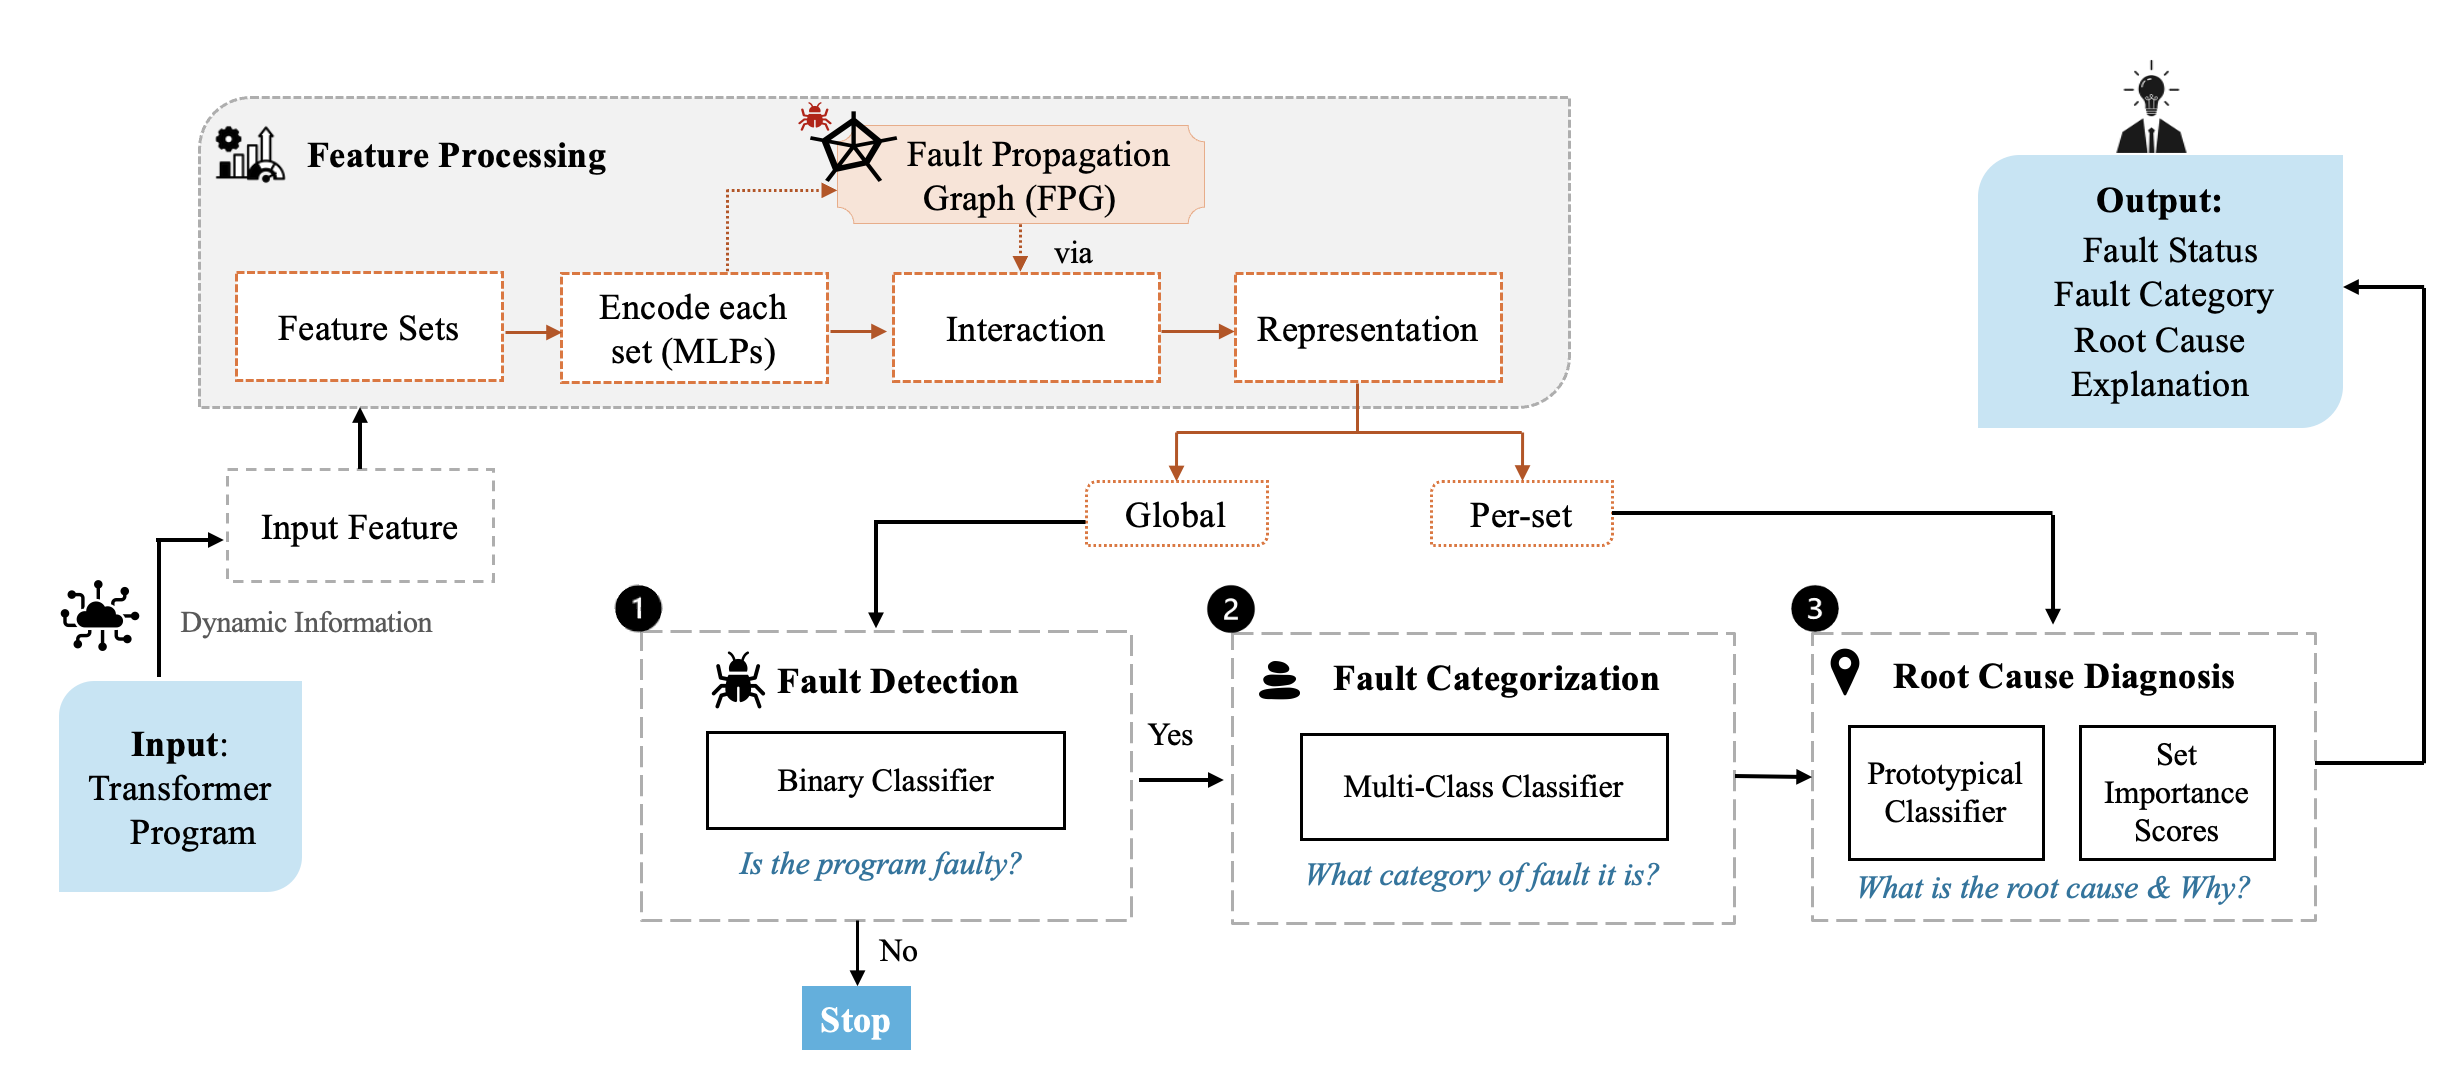
\includegraphics[width=\linewidth]{fig_method_overview.png}
\caption{Inference technique of DEFault++, showing the three-level diagnostic hierarchy from feature processing through fault detection, categorization, and root-cause diagnosis.}
\label{fig:defaultpp_technique}
\end{figure}

Algorithm~\ref{alg:defaultpp_inference} summarizes the diagnosis and explanation flow for one input instance. It shows the three-level gating logic and the explanation derivation; the shared encoding is defined in Sections~\ref{sec:defaultpp_encoding}--\ref{sec:defaultpp_message_passing}.

\begin{algorithm}[!htbp]
\caption{DEFault++ hierarchical diagnosis for one input instance}
\label{alg:defaultpp_inference}
\begin{algorithmic}[1]
\Statex \textbf{Input:} Feature vector $\mathbf{x}$; shared encoder producing group embeddings $\{\mathbf{h}_g\}_{g=1}^{G}$ and projection $\mathbf{z}_{\text{proj}}$; trained prototypes $\{\symbf{\pi}_{c,r}\}$
\Statex \textbf{Output:} Detection label $\hat{y}$; if faulty: fault category $\hat{c}$, root cause $\hat{r}$, and per-group importance scores $\{w_g\}_{g=1}^{G}$
\Statex
\Statex \textbf{Level 1 --- Fault Detection}
\State Classify the instance as faulty or clean: $\hat{y} \gets \text{Detect}(\mathbf{z}_{\text{proj}})$
\If{$\hat{y} = \textit{clean}$}
    \State \Return $\hat{y}$ \Comment{clean instances exit here; Levels~2--3 are not called}
\EndIf
\Statex
\Statex \textbf{Level 2 --- Fault Categorization}
\State Assign the fault to a transformer component category: $\hat{c} \gets \text{Categorize}(\mathbf{z}_{\text{proj}})$
\Statex
\Statex \textbf{Level 3 --- Root-Cause Diagnosis}
\For{each root cause $r$ in the predicted category $\mathcal{R}_{\hat{c}}$}
    \State Sum squared distances to prototype $r$ across all feature groups: $d_r \gets \sum_{g=1}^{G} \lVert \mathbf{h}_g - \symbf{\pi}_{\hat{c},r,g} \rVert^2$
\EndFor
\State Select the nearest prototype as the predicted root cause: $\hat{r} \gets \arg\min_{r \in \mathcal{R}_{\hat{c}}}\; d_r$
\Statex
\Statex \textbf{Explanation}
\State Identify the nearest alternative root cause: $\tilde{r} \gets \arg\min_{r \in \mathcal{R}_{\hat{c}} \setminus \{\hat{r}\}}\; d_r$
\For{each feature group $g = 1, \ldots, G$}
    \State Compute how much group $g$ favors $\hat{r}$ over $\tilde{r}$: $\Delta_g \gets d_g(\symbf{\pi}_{\hat{c},\tilde{r}}) - d_g(\symbf{\pi}_{\hat{c},\hat{r}})$
    \State Normalize positive contributions into importance score: $w_g \gets \max(\Delta_g,\,0)\;/\;\sum_{g'} \max(\Delta_{g'},\,0)$
\EndFor
\State \Return $\hat{y},\; \hat{c},\; \hat{r},\; \{w_g\}_{g=1}^{G}$
\end{algorithmic}
\end{algorithm}

\subsubsection{Feature-Group Encoding}
\label{sec:defaultpp_encoding}

We encode each feature group relying on a dedicated MLP. We keep groups structurally separated so that message passing in the Fault Propagation Graph can propagate information between them and so that the explanation step can examine each group's embedding independently. We use trainable MLPs rather than a flat classifier because the prototype-distance objective and the contrastive separation loss both require gradients to flow through the group-level weights during training. As encoder and decoder architectures differ in the number of feature groups ($G = 13$ vs.\ $G = 14$), we train separate encoder and decoder diagnostic models. Given the feature vector $\mathbf{z} \in \mathbb{R}^d$ partitioned into $G$ groups $\{\mathbf{z}_{g_1}, \ldots, \mathbf{z}_{g_G}\}$ (see Table~\ref{tab:defaultpp_features}), each group $g$ is encoded by a dedicated MLP (Equation~\ref{eq:group_encoding}).
\begin{equation}
\mathbf{h}_g = \text{MLP}_g(\mathbf{z}_g) \in \mathbb{R}^{h}, \quad g = 1, \ldots, G,
\label{eq:group_encoding}
\end{equation}
where $h = 32$ is the hidden dimension per group (selected via grid search on the inner validation fold). The group embeddings form the matrix $\mathbf{H} = [\mathbf{h}_1; \ldots; \mathbf{h}_G] \in \mathbb{R}^{G \times h}$.

A projection layer maps the concatenated group embeddings to a shared representation (Equation~\ref{eq:projection}).
\begin{equation}
\mathbf{z}_{\text{proj}} = W_{\text{proj}} \, \text{vec}(\mathbf{H}) \in \mathbb{R}^{e},
\label{eq:projection}
\end{equation}
where $e = 64$ is the embedding dimension and $\text{vec}(\mathbf{H}) \in \mathbb{R}^{Gh}$ denotes the row-major vectorization. Levels~1 and~2 use the pooled projection $\mathbf{z}_{\text{proj}}$ for detection and categorization. Level~3 uses the group embedding matrix $\mathbf{H}$ directly to preserve group-level structure for root-cause separation and group-level explanation (Section~\ref{sec:defaultpp_explainability}).

\subsubsection{Message Passing in the Fault Propagation Graph}
\label{sec:defaultpp_message_passing}

We update each group embedding by aggregating information from neighboring groups in the FPG. We construct the group-level adjacency matrix $\mathbf{A} \in \mathbb{R}^{G \times G}$ from the component-level FPG (Section~\ref{sec:defaultpp_fpg}) and the mapping in Table~\ref{tab:fpg_mapping}. Structural groups receive FPG-derived neighbor edges. The cross-layer observation group (Representation drift) and model-wide context groups (Training dynamics, Validation performance) receive self-loops only, meaning they undergo the learned transformation but do not aggregate information from neighboring groups. We compute updated group embeddings following graph convolutional networks~\cite{kipf2017semi}:
\begin{equation}
\mathbf{H}' = \operatorname{ReLU}\left(\hat{\mathbf{A}}\, \mathbf{H}\, W_{\text{msg}}\right),
\label{eq:message_passing}
\end{equation}
where $\hat{\mathbf{A}}$ is the row-normalized adjacency matrix (with self-loops) and $W_{\text{msg}} \in \mathbb{R}^{h \times h}$. We use row normalization rather than symmetric normalization because structural feature groups differ in the number of FPG propagation connections. Row normalization prevents high-degree groups from over-averaging their neighbors. The updated group embeddings $\mathbf{H}'$ replace the pre-message-passing $\mathbf{H}$ in both the projection and the Level~3 prototype matching. We apply three rounds of message passing, each with a dedicated learnable weight matrix. We selected the number of rounds via grid search on the inner validation fold (Appendix~\ref{app:defaultpp-parameters}).

For example, a QKV projection fault propagates to attention scores and the residual stream according to Mechanisms~1 and~2. Message passing along these edges aggregates that multi-group information into the QKV alignment embedding before classification. The model-wide context groups are transformed independently, without exchanging with neighbors, and contribute through the projection and prototype comparison steps.

\subsubsection{Hierarchical Classification}
\label{sec:defaultpp_stages}

All three classification levels share a single shared encoder (group encoding $+$ message passing in the FPG $+$ projection) rather than maintaining separate encoders per level. We use one shared encoder to reduce parameters and training cost. The computational cost of message passing over a 13/14-node group graph with 32-dimensional embeddings is itself negligible relative to the transformer training that produces the features, so including it in the shared pathway adds no meaningful overhead. The FPG also encodes structural dependencies between transformer components. A fault in one component (e.g., QKV projection) can shift measurements in downstream components (e.g., attention scores, residual stream). Message passing aggregates these cross-component dependencies into each group embedding, which benefits all three levels to varying degrees. Each level adds a task-specific head.

\paragraph{Level~1: Fault detection.}
A two-layer MLP maps $\mathbf{z}_{\text{proj}}$ to binary logits (faulty vs.\ correct).

\paragraph{Level~2: Fault categorization.}
A two-layer MLP maps $\mathbf{z}_{\text{proj}}$ to $C$-class logits, where $C = 11$ for encoders and $C = 12$ for decoders. During training, the class-weighted cross-entropy is computed only over samples labeled faulty.

\paragraph{Level~3: Root-cause diagnosis.}
Level~3 identifies 2--7 root causes within a fault category. Per-root-cause training support ranges from fewer than 10 samples (e.g., Variant encoder) to approximately 80, with an average of 42 per root cause for encoders and 26 for decoders. A standard softmax classifier risks overfitting to majority root causes in this regime. We therefore combine a cross-entropy head with a prototypical classifier~\cite{snell2017prototypical,kamp1995prototype}. The prototypical classifier needs fewer class-specific parameters by comparing each sample to class-mean embeddings rather than learning a separate weight vector per class.

First, a per-category classification head maps $\mathbf{z}_{\text{proj}}$ to root-cause logits within each category. During training, the cross-entropy loss is computed only over faulty samples whose ground-truth fault category matches the category under training. Negative samples for Level~3 are the other root causes within the same category, not samples from different categories. Second, a prototypical classifier~\cite{snell2017prototypical,lin2022prototypical} operates in the group embedding space $\mathbf{H} \in \mathbb{R}^{G \times h}$ (not the logit space). Distances in $\mathbf{H}$ are converted to class logits through the prototype-matching loss (Equation~\ref{eq:proto_matching}). Let $\mathcal{D}_{c,r}$ denote the set of training samples with category $c$ and root cause $r$. For each root cause $r$ within category $c$, we compute a prototype $\symbf{\pi}_{c,r}$ as the mean group embedding (Equation~\ref{eq:prototype}).
\begin{equation}
\symbf{\pi}_{c,r} = \frac{1}{|\mathcal{D}_{c,r}|} \sum_{i \in \mathcal{D}_{c,r}} \mathbf{H}_i \in \mathbb{R}^{G \times h}.
\label{eq:prototype}
\end{equation}

The distance from a sample to a prototype decomposes additively by group (Equation~\ref{eq:proto_distance}).
\begin{equation}
d(\mathbf{H}, \symbf{\pi}_{c,r}) = \sum_{g=1}^{G} \| \mathbf{h}_g - \symbf{\pi}_{c,r,g} \|^2 = \sum_{g=1}^{G} d_g,
\label{eq:proto_distance}
\end{equation}
where $d_g = \| \mathbf{h}_g - \symbf{\pi}_{c,r,g} \|^2$ is the squared distance contributed by group $g$.

Level~3 predicts the root cause whose prototype is nearest: $\hat{r} = \arg\min_{r \in \mathcal{R}_c} d(\mathbf{H}, \symbf{\pi}_{c,r})$. Because the distance decomposes additively by group (Equation~\ref{eq:proto_distance}), the prediction also admits a per-group explanation, which Section~\ref{sec:defaultpp_explainability} defines.

At inference time, Level~3 is called only after Level~2 predicts a fault category. Root-cause diagnosis is then restricted to that predicted category. The per-category cross-entropy heads are used only during training to provide auxiliary gradient information for the shared encoder. At inference, we use the prototype classifier because prototype distances decompose by group, which directly supports the group-level explanation in Section~\ref{sec:defaultpp_explainability}. The separation loss $\mathcal{L}_{\text{sep}}$ provides better separation within each category (Section~\ref{sec:defaultpp_training}).

\begin{figure}[!htbp]
\centering
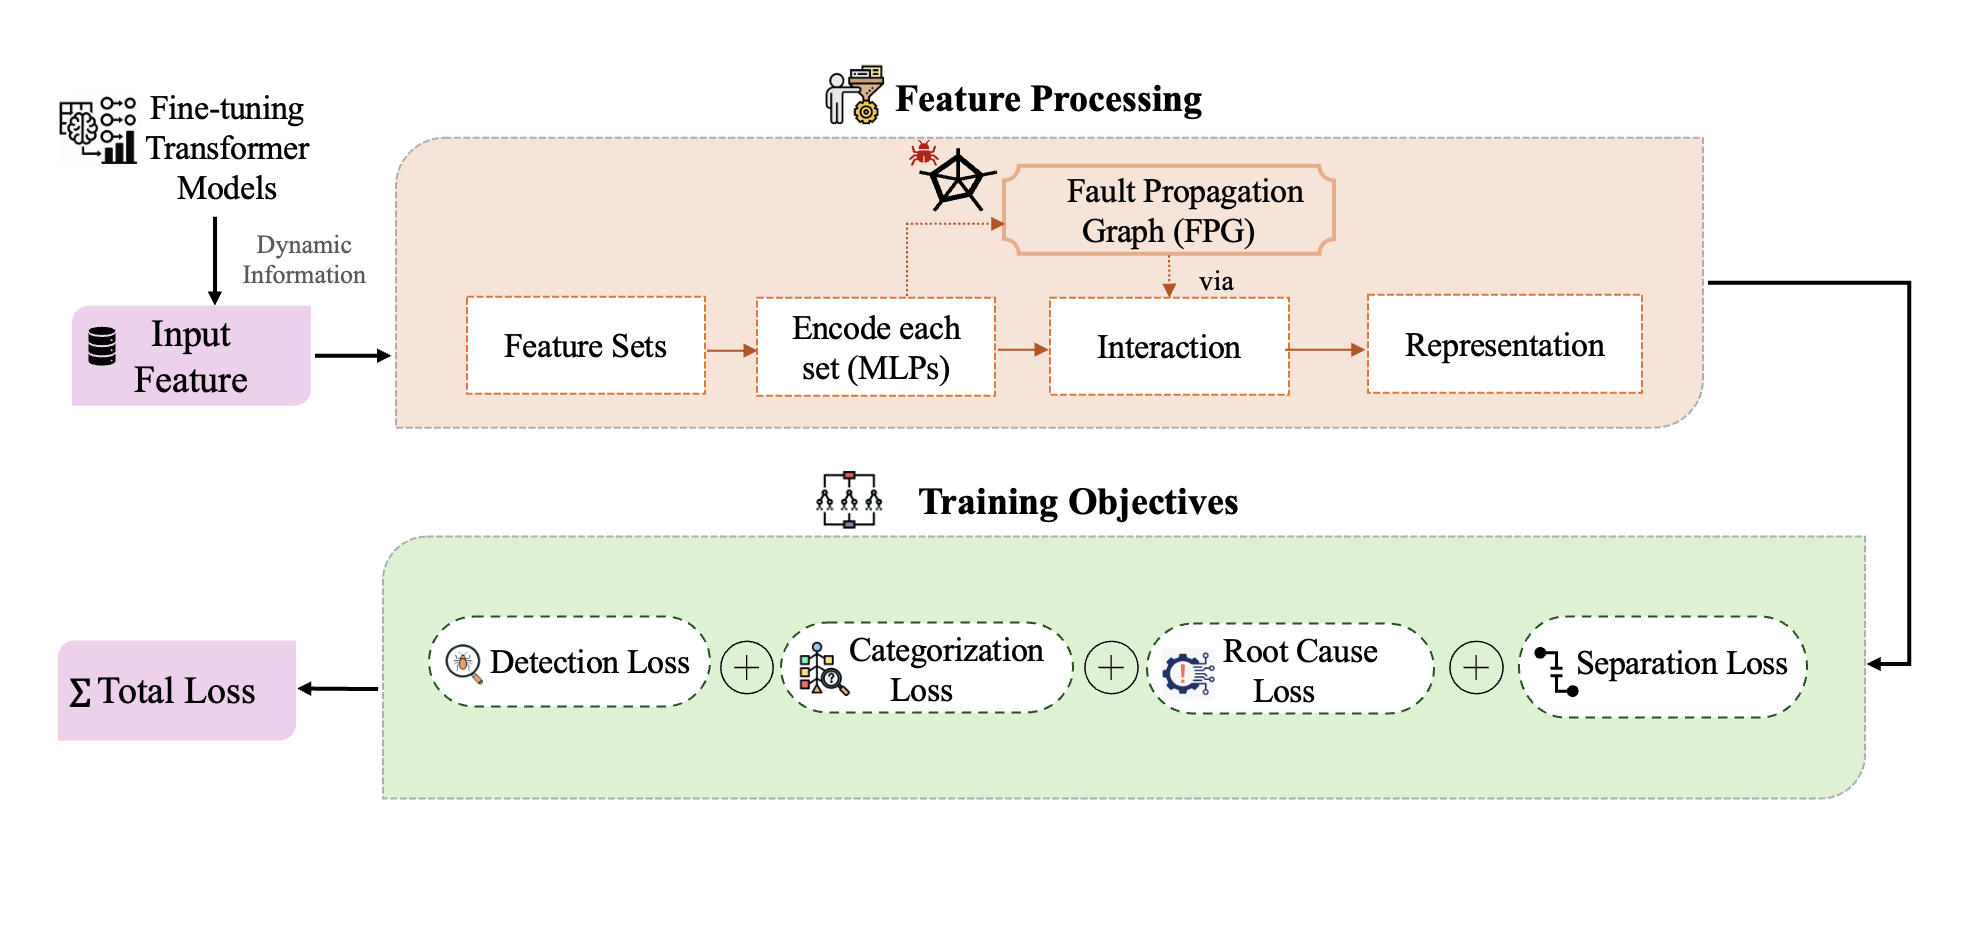
\includegraphics[width=\linewidth]{fig_training.png}
\caption{Training technique of DEFault++, showing the shared feature processing and the four loss components.}
\label{fig:defaultpp_training}
\end{figure}

\subsubsection{Training Objective}
\label{sec:defaultpp_training}

DEFault++ uses a hierarchical architecture at inference (Level~1 filters before Level~2, Level~2 filters before Level~3) but trains the shared encoding pathway jointly across all three levels. We adopt joint training with hard parameter sharing~\cite{caruana1997multitask,ruder2017overview} rather than training independent encoders per level. The dataset contains only 3{,}739 instances with an average of 42 samples per root cause for encoders and 26 for decoders (Section~\ref{sec:defaultpp_dataset}). Independent training would fragment this limited gradient information across separate encoders. Joint training is feasible because the three diagnostic tasks are nested: every Level~3 sample is also a Level~2 and Level~1 sample, and gradient directions across levels reinforce each other rather than opposing. The Level~2 categorization loss forces the encoder to produce category-separable embeddings, and the Level~3 separation loss forces within-category structure. Both constraints also improve Level~1 detection, since a more structured embedding space produces a cleaner binary boundary.

Each level uses a dedicated loss, and all losses are computed at the mini-batch level. Level~1 uses binary cross-entropy $\mathcal{L}_{\text{detect}}$ over all samples in the batch. Level~2 uses class-weighted cross-entropy $\mathcal{L}_{\text{cat}}$ over fault categories, applied to faulty samples only. Level~3 uses two losses jointly: per-category cross-entropy $\mathcal{L}_{\text{rc}}$ over root causes, and a root-cause separation loss $\mathcal{L}_{\text{sep}}$ that helps separate root causes within each category.

Cross-entropy trains per-category heads but does not explicitly structure the embedding space for within-category separation. We therefore define $\mathcal{L}_{\text{sep}}$ with two components. The first is a contrastive term that operates on the flattened group embeddings $\text{vec}(\mathbf{H})$. For each sample $i$ with category label $c_i$ and root-cause label $r_i$, positive pairs share both $(c_i, r_i)$, while negative pairs share $c_i$ but differ in root cause. Following supervised contrastive learning~\cite{khosla2020supervised}, the contrastive term within category $c$ is
\begin{equation}
\mathcal{L}_{\text{ctr}}^{(c)} = -\frac{1}{|\mathcal{P}_c|} \sum_{(i,j) \in \mathcal{P}_c} \log \frac{\exp(\text{sim}(\mathbf{h}_i, \mathbf{h}_j) / \tau)}{\sum_{k : c_k = c_i} \exp(\text{sim}(\mathbf{h}_i, \mathbf{h}_k) / \tau)},
\label{eq:contrastive}
\end{equation}
where $\mathcal{P}_c$ is the set of positive pairs within category $c$, $\text{sim}(\cdot, \cdot)$ is cosine similarity on the normalized flattened group embeddings, and $\tau = 0.1$ is the temperature. We use cosine similarity here because the contrastive objective targets directional alignment of embeddings, not their absolute magnitude~\cite{wang2021understanding,islam2023self}. The prototype classifier in Equation~\ref{eq:proto_distance} uses squared Euclidean distance instead, because prototype matching requires spatial proximity in the grouped embedding space rather than directional agreement.

We define the joint training objective $\mathcal{L}_{\text{DEFault++}}$ in Equation~\ref{eq:total_loss}.
\begin{equation}
\mathcal{L}_{\text{DEFault++}} = \mathcal{L}_{\text{detect}} + \alpha \, \mathcal{L}_{\text{cat}} + \lambda \, \mathcal{L}_{\text{rc}} + \mathcal{L}_{\text{sep}},
\label{eq:total_loss}
\end{equation}
where $\alpha$ and $\lambda$ are level-specific weighting coefficients. During training, we apply the root-cause separation loss $\mathcal{L}_{\text{sep}}$ only to faulty samples within their ground-truth fault category. At inference, Level~3 uses the predicted category from Level~2. The separation loss is defined as
\begin{equation}
\mathcal{L}_{\text{sep}} = \beta \, \mathcal{L}_{\text{ctr}} + \gamma \, \mathcal{L}_{\text{pm}},
\label{eq:separation_loss}
\end{equation}
where $\mathcal{L}_{\text{ctr}}$ is the contrastive term from Equation~\ref{eq:contrastive}, and $\mathcal{L}_{\text{pm}}$ is a prototype-matching loss defined as
\begin{equation}
\mathcal{L}_{\text{pm}} = -\frac{1}{|\mathcal{B}|} \sum_{i \in \mathcal{B}} \log \frac{\exp(-d(\mathbf{H}_i, \symbf{\pi}_{c_i, r_i}) / \tau_p)}{\sum_{r' \in \mathcal{R}_{c_i}} \exp(-d(\mathbf{H}_i, \symbf{\pi}_{c_i, r'}) / \tau_p)},
\label{eq:proto_matching}
\end{equation}
where $\mathcal{B}$ is the training batch, $d(\cdot, \cdot)$ is the grouped squared distance from Equation~\ref{eq:proto_distance}, $\mathcal{R}_{c_i}$ is the set of root causes within category $c_i$, and $\tau_p$ is a temperature parameter. By converting negative prototype distances into class logits, $\mathcal{L}_{\text{pm}}$ trains $\mathbf{H}$ so that the group-level distance gap (Equation~\ref{eq:group_contribution}) faithfully reflects the prediction.

We set $\alpha = 1.0$, $\lambda = 1.0$, $\beta = 0.5$, and $\gamma = 0.3$, where $\beta$ weights the contrastive term $\mathcal{L}_{\text{ctr}}$ and $\gamma$ weights the prototype-matching term $\mathcal{L}_{\text{pm}}$ in $\mathcal{L}_{\text{sep}}$. We selected all four coefficients via grid search on the inner validation fold (Appendix~\ref{app:defaultpp-parameters}). Training details appear in Section~\ref{sec:defaultpp_experiment}.

\subsubsection{FPG-Based Explanation}
\label{sec:defaultpp_explainability}

Level~3 predicts the root cause whose prototype is nearest in the grouped embedding space (Section~\ref{sec:defaultpp_stages}). To explain that prediction, we compare the predicted prototype $\symbf{\pi}_{c,\hat{r}}$ with the nearest alternative prototype $\symbf{\pi}_{c,\tilde{r}}$, where $\tilde{r} = \arg\min_{r \in \mathcal{R}_c \setminus \{\hat{r}\}} d(\mathbf{H}, \symbf{\pi}_{c,r})$. The distance gap between these two prototypes decomposes additively by group:
\begin{equation}
\Delta_g = d_g(\symbf{\pi}_{c,\tilde{r}}) - d_g(\symbf{\pi}_{c,\hat{r}}), \quad g = 1, \ldots, G,
\label{eq:group_contribution}
\end{equation}
where $d_g(\symbf{\pi}_{c,r}) = \| \mathbf{h}_g - \symbf{\pi}_{c,r,g} \|^2$. A positive $\Delta_g$ means group $g$ is closer to the predicted prototype than to the nearest alternative, so it favors the predicted root cause. A negative $\Delta_g$ means the group favors the alternative. The total gap $\sum_g \Delta_g$ equals the difference between the two full prototype distances, confirming that the decomposition is exact.

To summarize these contributions for visualization, we normalize the positive contributions into an importance score per group:
\begin{equation}
w_g = \frac{\max(\Delta_g, 0)}{\sum_{g'=1}^{G} \max(\Delta_{g'}, 0)}, \quad g = 1, \ldots, G.
\label{eq:explanation}
\end{equation}
Groups with negative contributions receive $w_g = 0$. The importance scores sum to one and highlight the groups that most support the predicted root cause.

For structural groups (Table~\ref{tab:fpg_mapping}), each $w_g$ maps directly to a transformer subsystem, so a large importance indicates which subsystem most supports the diagnosis after message passing~\cite{wolf2024keep}. For the cross-layer observation group (Representation drift), a large importance suggests that cross-layer representation drift is part of the diagnostic evidence, rather than a localized component effect. For model-wide context groups (Training dynamics, Validation performance), a large importance indicates model-wide deviation that corroborates the component-level diagnosis but does not localize the fault to a specific subsystem. Because $w_g$ is computed from distances in the post-message-passing embedding space, structural groups reflect fault effects as they propagate across components, while model-wide context groups reflect self-transformed embeddings without cross-group mixing. The group ablation in RQ$_3$ (Section~\ref{sec:defaultpp_rq3}) tests this interpretation by ablating the most important groups and measuring how much the gap decreases.


%==============================================================================
\section{Experiment}
\label{sec:defaultpp_experiment}

We evaluate DEFault++ on the test dataset. Encoder and decoder architectures are evaluated separately since their feature and label spaces differ.

\begin{rqlist}
\item \textbf{RQ$\mathbf{_1}$:} How does DEFault++ perform in detecting and categorizing transformer faults?
\item \textbf{RQ$\mathbf{_2}$:} How do message passing in the Fault Propagation Graph and the separation loss contribute to diagnostic performance?
\item \textbf{RQ$\mathbf{_3}$:} How does DEFault++ perform in root-cause diagnosis, and how faithful are the explanations?
\end{rqlist}

%------------------------------------------------------------------------------
\subsection{Evaluation Criteria}
\label{sec:defaultpp_cv}

We use nested grouped cross-validation with $k=5$ outer folds. We chose $k=5$ because the dataset contains only seven distinct (model, dataset) combinations, and five outer folds provide enough held-out groups per fold for stable Macro-F1 estimation while leaving sufficient training data for the inner loop. Instances are grouped by $(\text{model}, \text{dataset}, \text{seed})$ to prevent information leakage from correlated traces. The inner split uses \texttt{StratifiedGroupKFold} for model selection. The outer loop evaluates generalization on unseen groups, while the inner loop selects model hyperparameters. We restrict all preprocessing (e.g., scaling, thresholding, and standardization) and hyperparameter grid search strictly to the inner training fold. This design trains a total of 25 models per architecture (5~outer folds $\times$ 5~inner folds). Finally, we apply the outer fold assignments across all evaluated methods to ensure each method is evaluated on the same held-out samples. \footnote{Replication package: \url{https://github.com/SigmaJahan/DEFaultplusplus-Transformer-Debugging}}

We evaluate DEFault++ using four standard metrics. Let $\text{TP}$, $\text{FP}$, $\text{TN}$, and $\text{FN}$ denote the true positive, false positive, true negative, and false negative counts, respectively. Precision ($P$) and recall ($R$) are defined as
\begin{equation}
P = \frac{\text{TP}}{\text{TP} + \text{FP}}, \qquad R = \frac{\text{TP}}{\text{TP} + \text{FN}}.
\label{eq:prec_recall}
\end{equation}
The F1-score is the harmonic mean of precision and recall:
\begin{equation}
\text{F1} = \frac{2 \cdot P \cdot R}{P + R}.
\label{eq:f1}
\end{equation}
The class distributions are imbalanced at all three levels. We therefore report Macro-F1~\cite{naidu2023review}, which averages F1 across classes:
\begin{equation}
\text{Macro-F1} = \frac{1}{C} \sum_{c=1}^{C} \text{F1}_c,
\label{eq:macro_f1}
\end{equation}
where $C$ is the number of classes and $\text{F1}_c$ is the F1-score for class $c$. For fault detection (Level~1), we additionally report AUROC~\cite{bradley1997use}, which measures discriminative ability across all classification thresholds.

A true positive for fault detection means that a faulty configuration is correctly identified, regardless of its fault category. A true positive for fault categorization means that the category of the fault is identified correctly, regardless of the root cause. A true positive for root-cause diagnosis requires both the Level~2 category and the Level~3 root cause to be identified correctly in the same inference path.

\subsection{Implementation}

We implement the hierarchical model in PyTorch. We use separate MLPs for each feature group with hidden dimension $h = 32$ and a shared projection to $e = 64$ dimensions. We apply three rounds of message passing in the Fault Propagation Graph with the group-level adjacency matrix. Training uses Adam~\cite{kingma2015adam} with learning rate $10^{-3}$, weight decay $10^{-4}$, and batch size 256. We train for up to 150 epochs with early stopping on the validation split. The loss weights are $\alpha = 1.0$, $\lambda = 1.0$, $\beta = 0.5$, and $\gamma = 0.3$, with temperature $\tau = 0.1$. We address fault-category and root-cause imbalance through inverse-frequency weighting in the corresponding classification losses and select a fixed set of random seeds for reproducibility. Appendix~\ref{app:defaultpp-parameters} (Table~\ref{tab:defaultpp-hyperparameters}) gives the full hyperparameter configuration. The replication package~\cite{defaultpp_repo} contains the implementation, hyperparameter files, and trained models.

Training loss converges by ${\sim}$epoch 100, at which point validation Detection F1 and Category F1 also stabilize (Figures~\ref{fig:defaultpp_training_encoder} and~\ref{fig:defaultpp_training_decoder}). Training with early stopping at 150 epochs is sufficient for the three-level hierarchy.

\begin{figure}[!htbp]
\centering
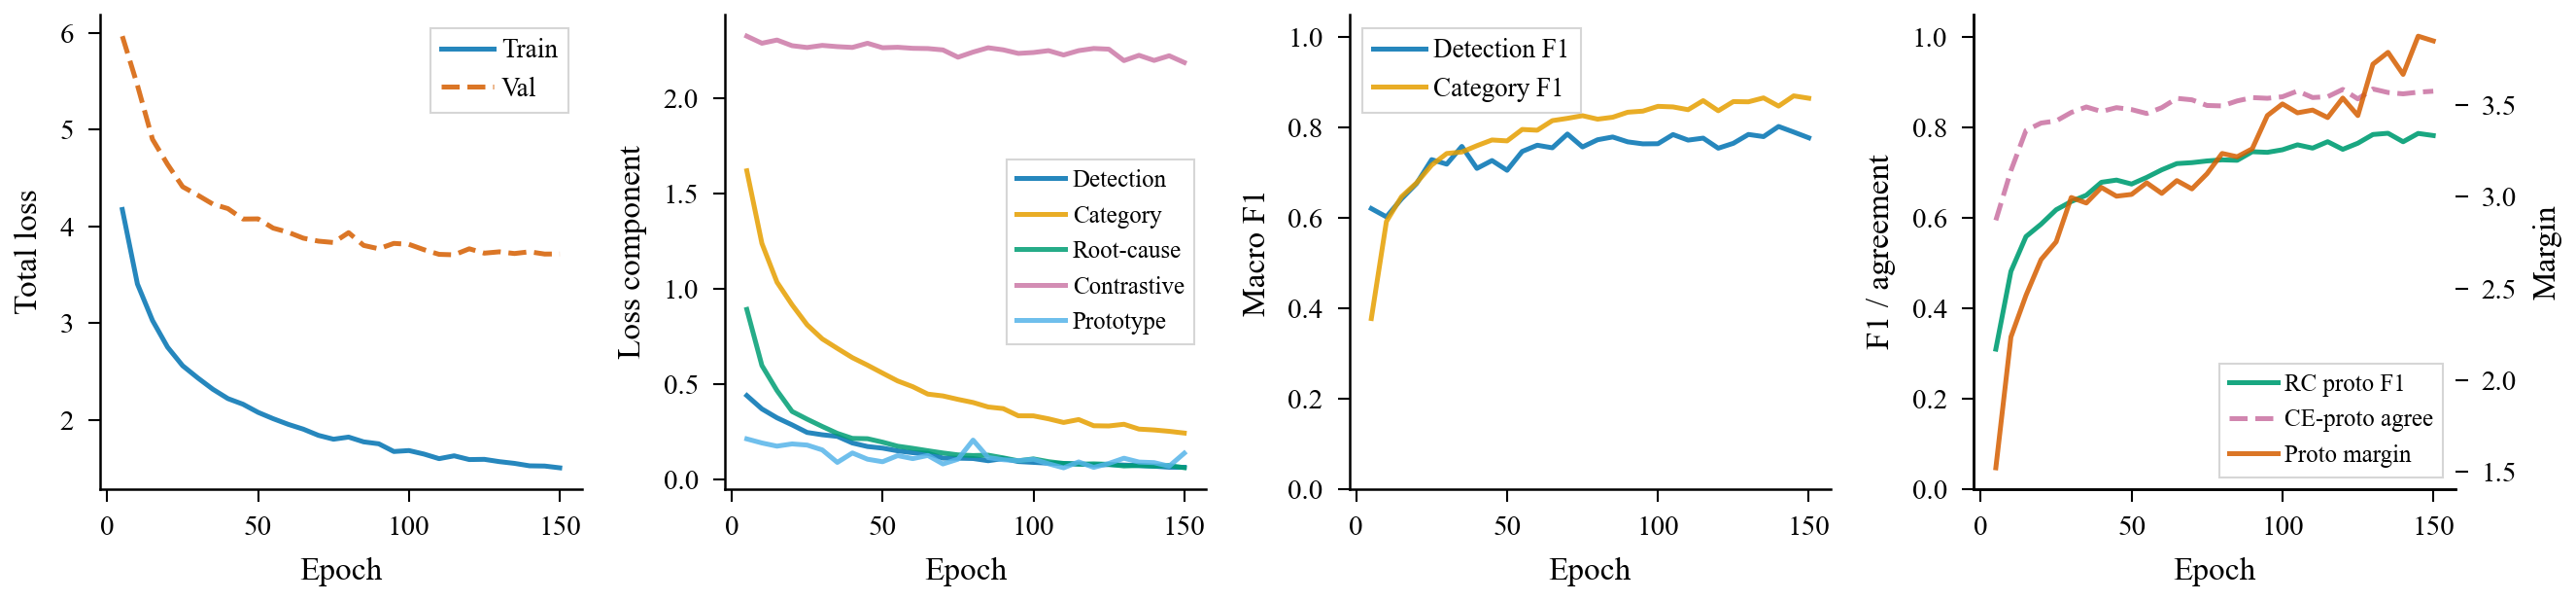
\includegraphics[width=0.9\linewidth]{fig_training_loss_encoder.png}
\caption{Training dynamics for DEFault++ on the encoder architecture.}
\label{fig:defaultpp_training_encoder}
\end{figure}

\begin{figure}[!htbp]
\centering
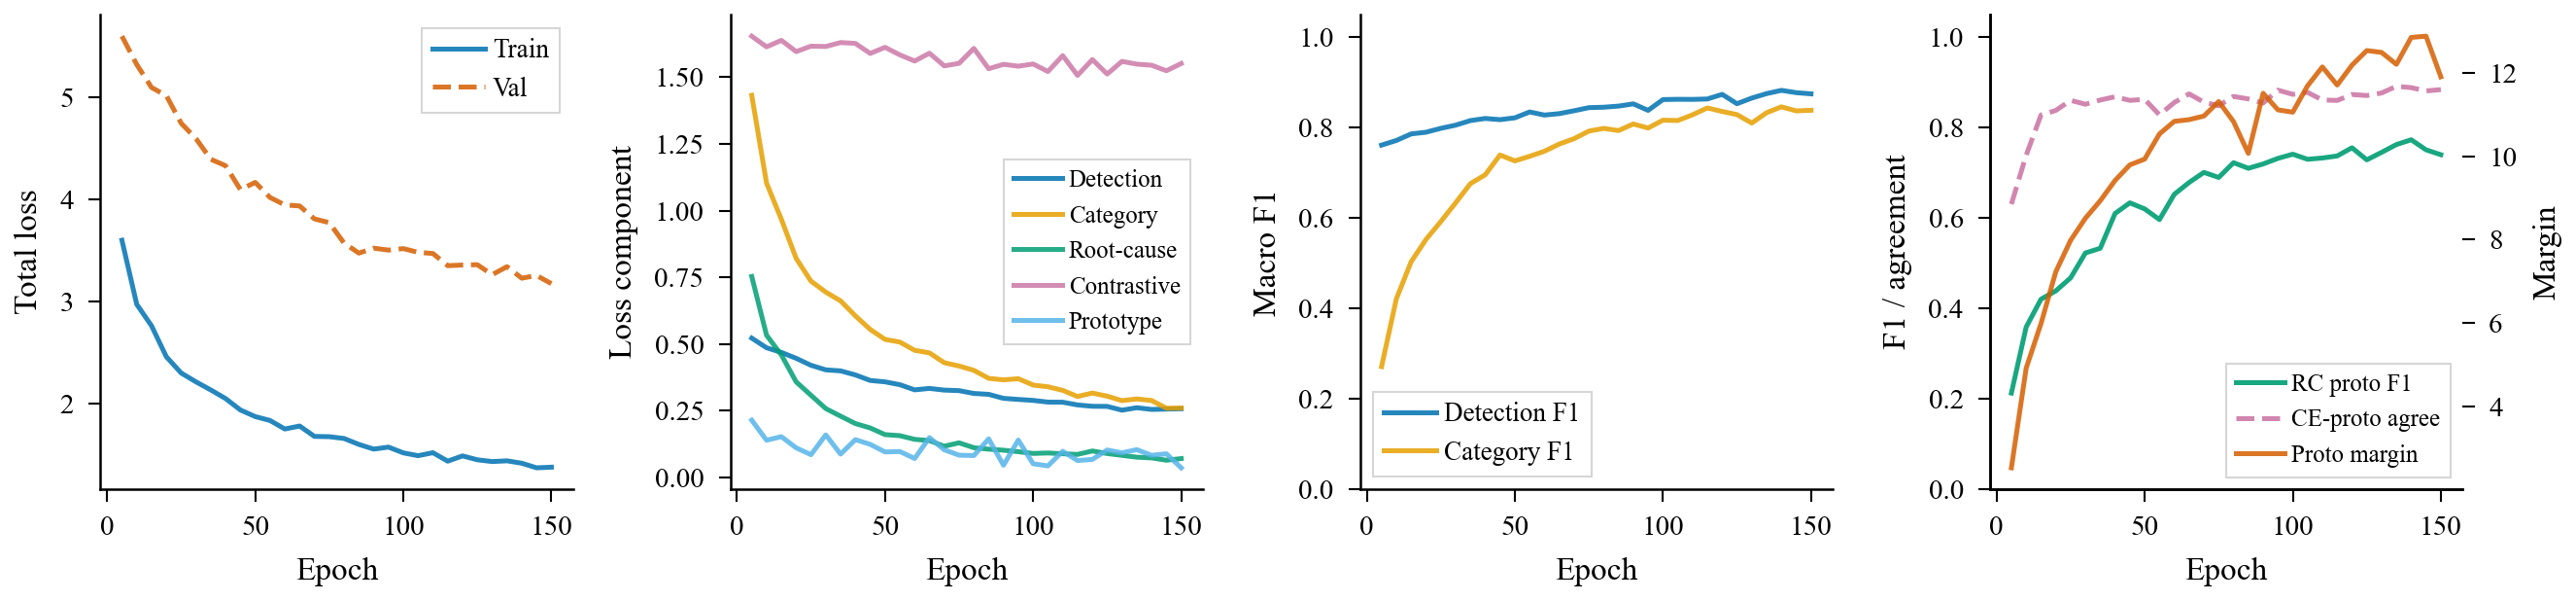
\includegraphics[width=0.9\linewidth]{fig_training_loss_decoder.png}
\caption{Training dynamics for DEFault++ on the decoder architecture.}
\label{fig:defaultpp_training_decoder}
\end{figure}

\subsection{Ablation Design}

We assess the contribution of each architectural component by systematically removing it from DEFault++ and measuring the performance drop. We ablate two components: message passing in the Fault Propagation Graph and the separation loss $\mathcal{L}_{\text{sep}}$. The separation loss applies only at Level~3. We define two variants for Levels~1 and~2 and four variants for Level~3:

\begin{enumerate}[nosep]
\item \textbf{DEFault++}. The complete model with message passing in the FPG and the separation loss at Level~3.
\item \textbf{$-$FPG}. We remove message passing in the FPG while retaining $\mathcal{L}_{\text{sep}}$ at Level~3. This variant measures the contribution of propagation-informed feature interaction.
\item \textbf{$-$Sep (Level~3 only)}. We remove the separation loss ($\beta = 0$, $\gamma = 0$) while retaining FPG. This variant measures the contribution of within-category root-cause discrimination.
\item \textbf{$-$FPG$-$Sep}. We remove both FPG and $\mathcal{L}_{\text{sep}}$, retaining only the feature-group MLPs with projection. This variant tests the hierarchical classifier alone.
\end{enumerate}

To test whether the specific FPG topology matters beyond just having any graph structure, we define two additional topology variants as follows.

\begin{enumerate}[nosep]
\item \textbf{Rewired}. We keep the same number of nodes and edges as the FPG but randomly reassign edge endpoints while preserving the degree distribution, following the degree-preserving rewiring procedure of Maslov and Sneppen~\cite{maslov2002specificity}. This rewiring preserves the overall graph density and local connectivity profile while breaking the meaningful propagation links between transformer components.
\item \textbf{Random}. We replace the FPG with an Erd\H{o}s--R\'{e}nyi random graph~\cite{erdos1959random} with approximately the same edge density. This replacement removes both the meaningful propagation links and the degree structure of the original FPG.
\end{enumerate}

\subsection{Baseline Approaches}

We compare DEFault++ against four prior techniques only on the Level~1 detection task. The baselines are evaluated on the same train/test partition as DEFault++. Rule-based techniques are executed with their published rule definitions and thresholds after mapping the required observables to the closest available trace features in our dataset. AutoTrainer's gradient-threshold rules map to our Training dynamics group. DeepDiagnosis adds rules that partially overlap with the Attention and Score groups. Learned baselines are trained as binary detectors on the Level~1 labels of each outer-training fold using the model families provided in their replication packages~\cite{autotrainer,deepdiagnosis,deepfd,default}. We do not recalibrate published rule thresholds on our dataset, and we do not claim Level~2 or Level~3 comparability since their native label space does not map validly to our transformer component categories or root causes.

\begin{enumerate}[label=(\roman*),nosep]
\item \textbf{AutoTrainer}~\cite{autotrainer} monitors five training symptoms (vanishing gradient, exploding gradient, dying ReLU, oscillating loss, slow convergence) via threshold rules applied during training. We map each rule to the corresponding features in our dataset and apply the published thresholds without recalibration. AutoTrainer was able to produce binary detection decisions but its symptom types do not map to our fault categories.

\item \textbf{DeepDiagnosis}~\cite{deepdiagnosis} extends AutoTrainer to eight symptom rules (adding unchanged weights, saturated activation, and out-of-range output) with a decision tree that maps detected symptoms to seven fix types. We apply the same feature-mapping strategy and thresholds. Its symptom labels likewise do not map to our fault categories.

\item \textbf{DeepFD}~\cite{deepfd} combines KNN, Decision Tree, and Random Forest classifiers with union voting to diagnose faults from runtime features. Its five diagnosis classes (e.g., incorrect learning rate, wrong activation function) do not correspond to our fault categories. We evaluate DeepFD as a binary classifier for the fault detection only.

\item \textbf{DEFault}~\cite{default} (Chapter~\ref{chapter_default}) uses a hierarchical Random Forest classifier that combines static and dynamic features to detect and categorize faults across seven coarse DNN-level categories (learning rate, activation function, loss function, optimizer, layer configuration, regularization, data processing). These categories operate at a different abstraction level. We evaluate DEFault for binary detection only.
\end{enumerate}

Table~\ref{tab:baseline_coverage} summarizes the coverage of each technique across our diagnostic levels.

\begin{table}[!htbp]
\caption{Baseline technique's coverage across DEFault++ diagnostic levels.}
\label{tab:baseline_coverage}
\centering
\footnotesize
\setlength{\tabcolsep}{4pt}
\begin{tabular}{@{} l l c c c @{}}
\toprule
\textbf{Technique} & \textbf{Paradigm} & \textbf{Detection} & \textbf{Categorization} & \textbf{Root-Cause} \\
\midrule
AutoTrainer~\cite{autotrainer}     & Rule-based (5 rules)      & \cmark & N/A & N/A \\
DeepDiagnosis~\cite{deepdiagnosis} & Rule-based (8 rules)      & \cmark & N/A & N/A \\
DeepFD~\cite{deepfd}               & Flat ensemble (KNN+DT+RF) & \cmark & N/A & N/A \\
DEFault~\cite{default}             & Hierarchical RF            & \cmark & N/A & N/A \\
\midrule
\textbf{DEFault++}          & Neural hierarchical        & \cmark & \cmark & \cmark \\
\bottomrule
\end{tabular}
\end{table}

%------------------------------------------------------------------------------
\subsection{Evaluation of DEFault++}

\subsubsection{\textbf{RQ$\mathbf{_1}$:} Fault Detection, Fault Categorization, and Baseline Comparison}
\label{sec:defaultpp_rq1}

\paragraph{Fault detection.}
Following the three-level hierarchy in Figure~\ref{fig:defaultpp_technique}, we first evaluate DEFault++ on binary fault detection (Level~1) across the nine tasks in the FrankenFormer benchmark~\cite{frankenformer}. The encoder tasks are five GLUE classification benchmarks\footnote{\url{https://gluebenchmark.com/}} (SST-2 for sentiment, QNLI for natural language inference, RTE for textual entailment, MRPC for paraphrase detection, and QQP for duplicate question detection). The decoder tasks are four language-modeling corpora (LAMBADA\footnote{\url{https://zenodo.org/record/2630551}} for word prediction, PTB\footnote{\url{https://catalog.ldc.upenn.edu/LDC99T42}} for Penn Treebank, WikiText-2\footnote{\url{https://huggingface.co/datasets/Salesforce/wikitext}}, and OpenWebText\footnote{\url{https://huggingface.co/datasets/Skylion007/openwebtext}}). DEFault++ achieves AUROC of 0.966 on encoders and 0.962 on decoders (Table~\ref{tab:perf_level1}). Detection recall of 0.852 (encoder) and 0.906 (decoder) indicates that DEFault++ identifies most faulty configurations before they reach Level~2. Figure~\ref{fig:defaultpp_roc} shows the detection ROC curves for both architectures.

\begin{table}[!htbp]
\centering
\caption{DEFault++ performance on fault detection (Level~1).}
\label{tab:perf_level1}
\begin{tabular}{l c c}
\toprule
\textbf{Metric} & \textbf{Encoder} & \textbf{Decoder} \\
\midrule
AUROC & 0.9660 & 0.9620 \\
Accuracy & 0.9455 & 0.9107 \\
Macro-F1 & 0.8238 & 0.9088 \\
Weighted-F1 & 0.9477 & 0.9104 \\
Precision & 0.8014 & 0.9125 \\
Recall & 0.8520 & 0.9064 \\
\bottomrule
\end{tabular}
\end{table}

\paragraph{Fault categorization.}
We evaluate DEFault++ on fault categorization (Level~2). DEFault++ achieves Macro-F1 of 0.850 on encoders and 0.868 on decoders (Table~\ref{tab:perf_level2_overall}). Categorization precision and recall remain balanced (0.866/0.840 for encoders, 0.879/0.865 for decoders), which indicates that the model does not sacrifice one for the other. Table~\ref{tab:rq1_perclass} breaks down categorization performance by fault category.

\begin{table}[!htbp]
\centering
\caption{DEFault++ performance on fault categorization (Level~2).}
\label{tab:perf_level2_overall}
\begin{tabular}{l c c}
\toprule
\textbf{Metric} & \textbf{Encoder} & \textbf{Decoder} \\
\midrule
Accuracy & 0.8522 & 0.8842 \\
Macro-F1 & 0.8497 & 0.8679 \\
Weighted-F1 & 0.8531 & 0.8850 \\
Precision & 0.8662 & 0.8794 \\
Recall & 0.8403 & 0.8649 \\
\bottomrule
\end{tabular}
\end{table}

\begin{table}[!htbp]
\centering
\caption{Per-category categorization performance for DEFault++.}
\label{tab:rq1_perclass}
\small
\begin{tabular}{l c c c c c c}
\toprule
& \multicolumn{3}{c}{\textbf{Encoder}} & \multicolumn{3}{c}{\textbf{Decoder}} \\
\cmidrule(lr){2-4} \cmidrule(lr){5-7}
\textbf{Category} & \textbf{F1} & \textbf{Prec.} & \textbf{Rec.} & \textbf{F1} & \textbf{Prec.} & \textbf{Rec.} \\
\midrule
Embedding & 0.838 & 0.852 & 0.829 & 0.862 & 0.833 & 0.897 \\
FFN & 0.836 & 0.807 & 0.871 & 0.718 & 0.673 & 0.777 \\
Kernel & 0.771 & 0.814 & 0.740 & 0.765 & 0.848 & 0.700 \\
KV Cache & --- & --- & --- & 0.758 & 0.716 & 0.822 \\
LayerNorm & 0.790 & 0.775 & 0.820 & 0.843 & 0.937 & 0.766 \\
Masking & 0.917 & 0.952 & 0.886 & 0.890 & 0.927 & 0.857 \\
Output & 0.889 & 0.927 & 0.864 & 0.975 & 0.980 & 0.969 \\
Positional & 0.919 & 0.950 & 0.891 & 0.927 & 0.949 & 0.911 \\
QKV & 0.825 & 0.863 & 0.792 & 0.789 & 0.772 & 0.815 \\
Residual & 0.961 & 0.965 & 0.958 & 0.995 & 0.995 & 0.995 \\
Score & 0.861 & 0.847 & 0.876 & 0.946 & 0.937 & 0.957 \\
Variant & 0.741 & 0.776 & 0.717 & 0.948 & 0.986 & 0.914 \\
\midrule
\textbf{Macro avg.} & 0.850 & 0.866 & 0.840 & 0.868 & 0.879 & 0.865 \\
\bottomrule
\end{tabular}
\end{table}

We identify Residual and Positional as the strongest fault categories. Residual achieves near-perfect F1 on both architectures (0.961 encoder, 0.995 decoder), as the Residual stream group produces separable skip-connection measurements for these fault categories. On encoders, Variant (0.741) and Kernel (0.771) report the lowest F1. On decoders, FFN (0.718) and KV Cache (0.758) are the most difficult. We also observe that Variant differs sharply across architectures (F1 0.741 encoder vs.\ 0.948 decoder). One plausible explanation is that encoder Variant faults have only 24 instances (Table~\ref{tab:data_accounting}), the smallest category, while decoder Variant faults have 51 instances and benefit from stronger cache-related discriminative features. Figure~\ref{fig:defaultpp_roc} shows the detection ROC curves.

\begin{figure}[!htbp]
\centering
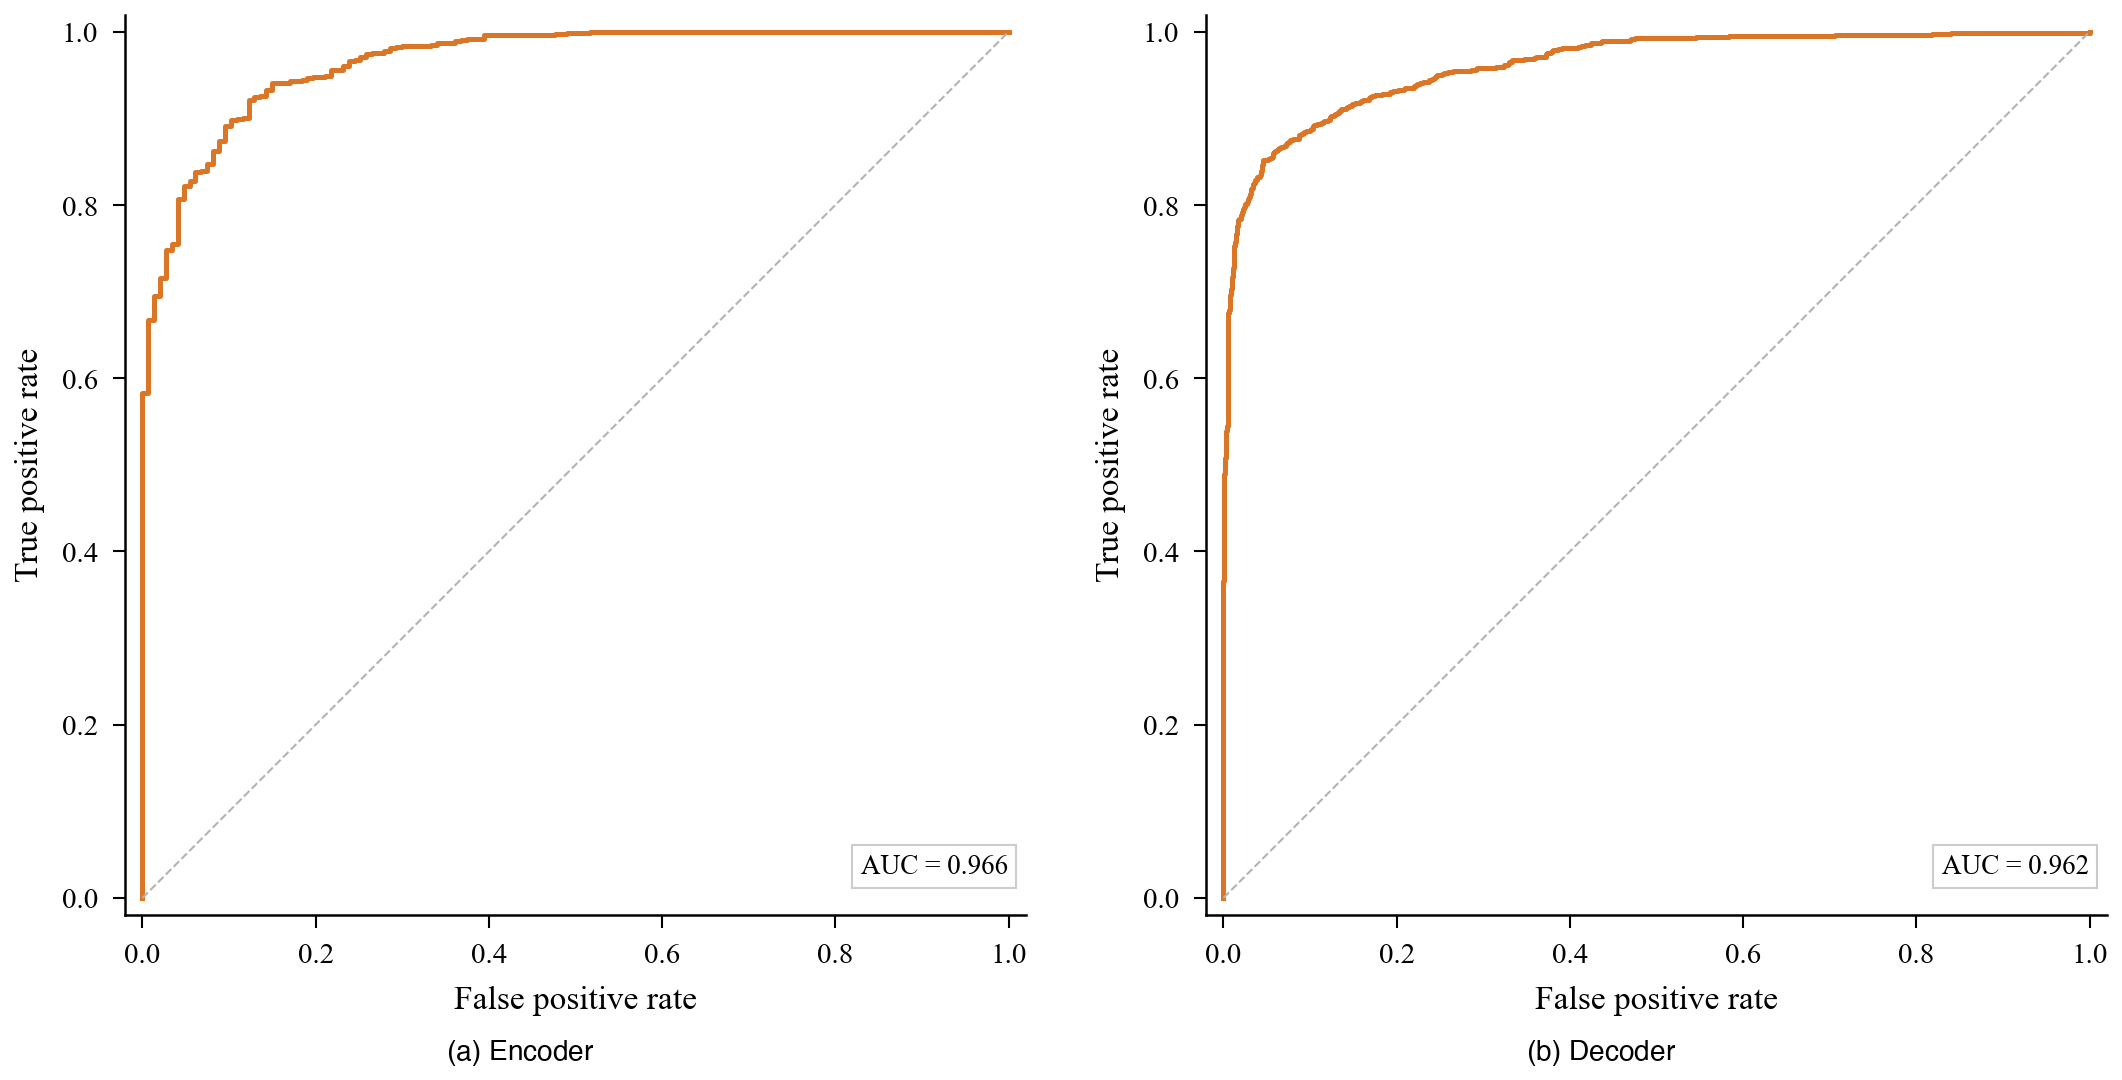
\includegraphics[width=0.9\linewidth]{fig_RQ1_roc_detection.png}
\caption{ROC curves for fault detection on encoder and decoder architectures.}
\label{fig:defaultpp_roc}
\end{figure}

\FloatBarrier

\paragraph{Baseline comparison.}
We compare DEFault++ against four baselines on the binary detection task (Table~\ref{tab:rq1_detection_comparison}). DEFault++ achieves the highest AUROC on both architectures (0.9660 encoder, 0.9620 decoder). DEFault reaches 0.8610 on encoders and 0.9030 on decoders. DeepFD reaches 0.8340 and 0.8810 respectively. Both learned methods score above the threshold-based methods. Macro-F1 follows the same ranking. DEFault++ reaches 0.8238 on encoders and 0.9088 on decoders. DEFault reaches 0.5660 and 0.7020. DeepFD reaches 0.5140 and 0.6550.

DEFault and DeepFD can still separate faulty from correct transformer models, as binary detection does not require alignment with the 11/12 transformer component categories. We attribute their lower scores to the feature space each method uses. DEFault relies on a hierarchical random forest over general DNN behavioral features, which detects broad fault patterns but does not model transformer-specific structures such as attention distributions or projection alignments. DeepFD uses a flat ensemble over DNN-level fault categories, which lacks the specificity to detect faults that manifest in transformer-specific components.

AutoTrainer and DeepDiagnosis produce the lowest Macro-F1 scores. AutoTrainer reaches 0.2840 on encoders and 0.4270 on decoders. DeepDiagnosis reaches 0.3380 and 0.4820. Both methods apply fixed threshold rules over generic DNN training symptoms. AutoTrainer encodes five such rules and DeepDiagnosis eight, none of which targets the attention, projection, or cache behaviors that characterize faults in transformer architectures.

\begin{table*}[!htbp]
\centering
\caption{Fault-detection comparison between DEFault++ and baselines.}
\label{tab:rq1_detection_comparison}
\footnotesize
\begin{adjustbox}{max width=\textwidth}
\begin{tabular}{l l c c c c c c}
\toprule
\textbf{Method} & \textbf{Type} & \textbf{AUROC (Enc)} & \textbf{M-F1 (Enc)} & \textbf{Acc.\ (Enc)} & \textbf{AUROC (Dec)} & \textbf{M-F1 (Dec)} & \textbf{Acc.\ (Dec)} \\
\midrule
\textbf{DEFault++} & Neural hierarchical & $\mathbf{0.9660}$ & $\mathbf{0.8238}$ & $\mathbf{0.9455}$ & $\mathbf{0.9620}$ & $\mathbf{0.9088}$ & $\mathbf{0.9107}$ \\
DEFault~\cite{default} & Hierarchical RF & $0.8610$ & $0.5660$ & $0.8120$ & $0.9030$ & $0.7020$ & $0.8460$ \\
DeepFD~\cite{deepfd} & Flat ensemble & $0.8340$ & $0.5140$ & $0.7810$ & $0.8810$ & $0.6550$ & $0.8190$ \\
DeepDiagnosis~\cite{deepdiagnosis} & Rule-based (8 rules) & --- & $0.3380$ & $0.7240$ & --- & $0.4820$ & $0.7710$ \\
AutoTrainer~\cite{autotrainer} & Rule-based (5 rules) & --- & $0.2840$ & $0.6970$ & --- & $0.4270$ & $0.7440$ \\
\bottomrule
\end{tabular}
\end{adjustbox}

\smallskip
\noindent{\footnotesize Rule-based techniques produce binary decisions without probabilistic scores. AUROC is therefore not applicable (---). All values are averaged over five outer folds. Learned methods are fit on the training portion of each outer fold, and rule-based methods are applied directly to the corresponding held-out fold.}
\end{table*}

We do not report Level~2 or Level~3 comparisons against these baselines. AutoTrainer and DeepDiagnosis generate generic symptom labels that do not map to any fault category in our taxonomy. DeepFD and DEFault use DNN-level fault categories that were defined independently of transformer component boundaries. A numeric comparison at those levels would equate non-equivalent labels, thus we report baseline coverage in Table~\ref{tab:baseline_coverage} instead.

\begin{rqsummary}
\textbf{Summary of RQ$\mathbf{_1}$:} DEFault++ outperforms existing fault detection techniques, achieving an AUROC above 0.96 and a Macro-F1 above 0.85 across both architectures. Residual and Positional categories score highest due to separable feature distributions, while Variant, Kernel, and FFN score lower due to limited support and overlapping distributions.
\end{rqsummary}

%------
\subsubsection{\textbf{RQ$\mathbf{_2}$:} Ablation Analysis}
\label{sec:defaultpp_rq2}

We examine the contribution of message passing in the Fault Propagation Graph and the separation loss through ablation. Tables~\ref{tab:abl_l1} and~\ref{tab:abl_l2} compare DEFault++ with and without message passing at Levels~1 and~2, where the separation loss does not apply. Table~\ref{tab:abl_l3} compares all four variants at Level~3.

\begin{table}[t]
\centering
\caption{Ablation study of Level~1: Fault Detection.}
\label{tab:abl_l1}
\small
\begin{tabular}{l l c c c c c c}
\toprule
\textbf{Arch.} & \textbf{Variant} & \textbf{AUROC} & \textbf{Acc.} & \textbf{F1} & \textbf{F1$_w$} & \textbf{Prec.} & \textbf{Rec.} \\
\midrule
Encoder & DEFault++ & 0.966 & 0.946 & 0.824 & 0.948 & 0.801 & 0.852 \\
        & $-$FPG & 0.921 & 0.922 & 0.782 & 0.924 & 0.752 & 0.816 \\
\midrule
Decoder & DEFault++ & 0.962 & 0.911 & 0.909 & 0.910 & 0.912 & 0.906 \\
        & $-$FPG & 0.949 & 0.892 & 0.890 & 0.892 & 0.890 & 0.891 \\
\bottomrule
\end{tabular}
\end{table}

\begin{table}[t]
\centering
\caption{Ablation study of Level~2: Fault Categorization.}
\label{tab:abl_l2}
\small
\begin{tabular}{l l c c c c c}
\toprule
\textbf{Arch.} & \textbf{Variant} & \textbf{Acc.} & \textbf{F1} & \textbf{F1$_w$} & \textbf{Prec.} & \textbf{Rec.} \\
\midrule
Encoder & DEFault++ & 0.852 & 0.850 & 0.853 & 0.866 & 0.840 \\
        & $-$FPG & 0.743 & 0.742 & 0.745 & 0.757 & 0.731 \\
\midrule
Decoder & DEFault++ & 0.884 & 0.868 & 0.885 & 0.879 & 0.865 \\
        & $-$FPG & 0.790 & 0.788 & 0.791 & 0.797 & 0.783 \\
\bottomrule
\end{tabular}
\end{table}

\begin{table}[t]
\centering
\caption{Ablation study of Level~3: Root Cause Diagnosis.}
\label{tab:abl_l3}
\small
\begin{tabular}{l l c c c c c}
\toprule
\textbf{Arch.} & \textbf{Variant} & \textbf{Acc.} & \textbf{F1} & \textbf{F1$_w$} & \textbf{Prec.} & \textbf{Rec.} \\
\midrule
Encoder & DEFault++ & 0.795 & 0.851 & 0.857 & 0.941 & 0.793 \\
        & $-$FPG & 0.778 & 0.812 & 0.819 & 0.933 & 0.776 \\
        & $-$Sep & 0.752 & 0.756 & 0.763 & 0.910 & 0.752 \\
        & $-$FPG$-$Sep & 0.702 & 0.701 & 0.711 & 0.883 & 0.690 \\
\midrule
Decoder & DEFault++ & 0.826 & 0.867 & 0.875 & 0.948 & 0.823 \\
        & $-$FPG & 0.810 & 0.833 & 0.840 & 0.940 & 0.809 \\
        & $-$Sep & 0.781 & 0.781 & 0.788 & 0.925 & 0.781 \\
        & $-$FPG$-$Sep & 0.735 & 0.734 & 0.742 & 0.896 & 0.721 \\
\bottomrule
\end{tabular}
\end{table}

We apply message passing in the Fault Propagation Graph as part of the shared encoding pathway across all three levels, following standard multi-task practice where lower representation layers are shared across tasks. We discuss the ablation results at each level.

\paragraph{Level~1: Fault detection.} We find that removing message passing in the FPG modestly reduces detection performance on both architectures (Table~\ref{tab:abl_l1}). Binary detection is a coarse task. A fault that disrupts any transformer component shifts the overall feature distribution enough for the binary classifier to separate faulty from clean configurations. The classifier does not need to determine which component failed or how the fault propagated. We observe that message passing adds cross-group information that improves the binary boundary, but the group-level features alone already support detection. We retain message passing at Level~1 because the cross-component aggregation helps detect faults with weak local deviations, and the ablation confirms that removing it reduces rather than improves detection.

\paragraph{Level~2: Fault categorization.} We find that removing message passing in the FPG produces the largest drop in the entire ablation (Table~\ref{tab:abl_l2}). Categorization requires the classifier to distinguish between 11/12 fault categories, several of which affect overlapping feature groups. A QKV fault propagates to attention scores and the residual stream. A Score fault propagates to attention weights and onward to the residual stream, but through a narrower path than a QKV fault, which simultaneously affects both scores and values. Without message passing, we compute each group embedding independently, and the classifier can only infer cross-group relationships from the flat projection. With message passing, we route fault evidence along the FPG propagation edges before the projection step, producing representations that already encode how the fault spreads across components. We attribute the large drop to this loss of cross-group structure, because the propagation pattern is what distinguishes categories with overlapping features.

\paragraph{Level~3: Root-cause diagnosis.} We ablate both the separation loss and message passing independently at Level~3 (Table~\ref{tab:abl_l3}). We find that removing the separation loss produces the larger drop. Root causes within the same fault category share much of the same feature distribution because they affect the same transformer component. A weight-corruption fault and a stale-parameter fault both appear in the QKV feature group with similar aggregate patterns. Cross-entropy alone does not explicitly structure the embedding space to separate these closely positioned root causes. We designed the separation loss to address this gap by pulling same-root-cause embeddings together and pushing different-root-cause embeddings apart within each category.

We find that removing message passing in the FPG at Level~3 (while retaining the separation loss) produces a smaller drop. Message passing aggregates propagation-related evidence across groups before prototype comparison, but the root-cause discrimination problem centers on within-category separation rather than cross-group structure. We observe that removing both components together produces the largest overall drop, which confirms that message passing and the separation loss contribute complementary information at Level~3.

\paragraph{Topology ablation.} The preceding ablation compares the full FPG with no message passing at all. To test whether the specific FPG topology matters, we compare it with two alternative graph structures: Rewired (same density, shuffled edges) and Random (Erd\H{o}s--R\'{e}nyi graph with matched density). Table~\ref{tab:abl_topology} reports Macro-F1 across all three levels.

\begin{table}[t]
\centering
\caption{Topology ablation: Macro-F1 across graph variants.}
\label{tab:abl_topology}
\small
\begin{tabular}{@{} l l c c c c @{}}
\toprule
\textbf{Level} & \textbf{Arch.} & \textbf{DEFault++} & \textbf{Rewired} & \textbf{Random} & \textbf{$-$FPG} \\
\midrule
L1 & Encoder & 0.824 & 0.790 & 0.786 & 0.782 \\
   & Decoder & 0.909 & 0.894 & 0.892 & 0.890 \\
\midrule
L2 & Encoder & 0.850 & 0.770 & 0.754 & 0.742 \\
   & Decoder & 0.868 & 0.807 & 0.796 & 0.788 \\
\midrule
L3 & Encoder & 0.851 & 0.820 & 0.816 & 0.812 \\
   & Decoder & 0.867 & 0.838 & 0.835 & 0.833 \\
\bottomrule
\end{tabular}
\end{table}

The results show a consistent ordering at every level and on both architectures: DEFault++ $>$ Rewired $>$ Random $>$ $-$FPG. The FPG with the correct propagation structure outperforms both alternative topologies. Rewired edges preserve the graph density and degree distribution but break the meaningful propagation links, and the performance drops below the full FPG at every level. Random edges lose both the specific links and the degree structure of the original FPG, and performance drops further. Removing message passing entirely ($-$FPG) produces the lowest performance.

The topology effect is strongest at Level~2, where DEFault++ outperforms Rewired by 0.080 (encoder) and 0.061 (decoder) in Macro-F1. This is consistent with the earlier finding that fault categorization depends most on cross-group propagation structure. At Level~1 and Level~3, the topology differences are smaller because binary detection is a coarser task and root-cause diagnosis depends more on within-category separation than on cross-group structure.

\FloatBarrier

\begin{rqsummary}
\textbf{Summary of RQ$\mathbf{_2}$:} DEFault++ adds two architectural components beyond the base DEFault hierarchical model: FPG message passing and root-cause separation loss. Removing message passing in the Fault Propagation Graph reduces performance at all three levels. The largest impact appears at Level~2 categorization, where cross-group propagation structure is essential for distinguishing fault categories with overlapping features. At Level~3, removing the separation loss produces the largest single-component drop, because root-cause discrimination requires explicit within-category separation that cross-entropy alone does not enforce. A topology ablation further confirms that the specific FPG structure matters: both rewired and random graphs underperform the correct propagation topology at every level, with the largest gap at Level~2.
\end{rqsummary}

%------
\subsubsection{\textbf{RQ$\mathbf{_3}$:} Root-Cause Diagnosis and Explanation}
\label{sec:defaultpp_rq3}

At Level~3, DEFault++ identifies the specific root cause within the fault category predicted at Level~2. Each fault category contains 2--7 structurally distinct root causes, evaluated across the nine FrankenFormer benchmark tasks described in Section~\ref{sec:defaultpp_rq1}. DEFault++ separates these root causes at Macro-F1 of 0.851 on encoders and 0.867 on decoders, as reported in Tables~\ref{tab:perf_level3_overall} and~\ref{tab:perf_level3_category}.

\begin{table}[!htbp]
\centering
\caption{DEFault++ performance on hierarchical root-cause diagnosis.}
\label{tab:perf_level3_overall}
\begin{tabular}{l c c}
\toprule
\textbf{Metric} & \textbf{Encoder} & \textbf{Decoder} \\
\midrule
Accuracy & 0.7953 & 0.8264 \\
Macro-F1 & 0.8512 & 0.8670 \\
Weighted-F1 & 0.8567 & 0.8745 \\
Precision & 0.9407 & 0.9475 \\
Recall & 0.7932 & 0.8225 \\
\bottomrule
\end{tabular}
\end{table}

\begin{table}[!htbp]
\centering
\caption{Per-category root-cause performance for DEFault++.}
\label{tab:perf_level3_category}
\small
\begin{tabular}{l c c c c c c c c}
\toprule
& \multicolumn{4}{c}{\textbf{Encoder}} & \multicolumn{4}{c}{\textbf{Decoder}} \\
\cmidrule(lr){2-5} \cmidrule(lr){6-9}
\textbf{Category} & \textbf{F1} & \textbf{Acc.} & \textbf{Prec.} & \textbf{Rec.} & \textbf{F1} & \textbf{Acc.} & \textbf{Prec.} & \textbf{Rec.} \\
\midrule
Embedding & 0.879 & 0.805 & 0.972 & 0.806 & 0.877 & 0.890 & 0.972 & 0.816 \\
FFN & 0.804 & 0.808 & 0.847 & 0.778 & 0.883 & 0.777 & 1.000 & 0.803 \\
Kernel & 0.814 & 0.740 & 1.000 & 0.706 & 0.747 & 0.691 & 0.988 & 0.676 \\
KV Cache & --- & --- & --- & --- & 0.881 & 0.822 & 1.000 & 0.817 \\
LayerNorm & 0.821 & 0.748 & 0.917 & 0.749 & 0.890 & 0.749 & 0.969 & 0.839 \\
Masking & 0.925 & 0.871 & 0.986 & 0.874 & 0.845 & 0.755 & 0.902 & 0.801 \\
Output & 0.882 & 0.825 & 0.958 & 0.822 & 0.972 & 0.969 & 1.000 & 0.947 \\
Positional & 0.930 & 0.884 & 0.992 & 0.886 & 0.975 & 0.911 & 1.000 & 0.953 \\
QKV & 0.765 & 0.693 & 0.868 & 0.694 & 0.646 & 0.629 & 0.727 & 0.592 \\
Residual & 0.908 & 0.880 & 0.927 & 0.895 & 0.958 & 0.955 & 0.961 & 0.955 \\
Score & 0.835 & 0.779 & 0.879 & 0.799 & 0.908 & 0.897 & 0.926 & 0.897 \\
Variant & 0.799 & 0.717 & 1.000 & 0.717 & 0.824 & 0.871 & 0.925 & 0.773 \\
\midrule
\textbf{Macro avg.} & 0.851 & 0.795 & 0.941 & 0.793 & 0.867 & 0.826 & 0.948 & 0.823 \\
\bottomrule
\end{tabular}
\end{table}

The strongest categories for root-cause diagnosis are Positional (0.930 encoder, 0.975 decoder), Masking (0.925 encoder, 0.845 decoder), and Residual (0.908 encoder, 0.958 decoder). Positional root causes produce distinct patterns in positional-sensitivity, attention-entropy, and pre-softmax score features. Residual root causes are distinguished because skip-connection integrity and gradient-norm features produce non-overlapping distributions across root causes within that category. QKV is the weakest category for root-cause separation, with F1 of 0.765 on encoders and 0.646 on decoders. QKV root causes activate overlapping feature groups because multiple root causes within the category affect projection weights, alignment measurements, and update flow measurements simultaneously. The shared activation patterns limit the margin the prototype-matching loss can enforce between root causes.

Root-cause count alone does not explain this pattern. Residual remains strong despite five root causes because its skip-connection and gradient features are well separated, whereas QKV is the weakest category even with four root causes because three of the four root causes disturb the same projection and alignment measurements. This pattern suggests that per-category difficulty depends more on feature separability than on the number of root causes by itself.

The per-category metrics in Table~\ref{tab:perf_level3_category} measure how well Level~3 separates root causes once the fault category is fixed. They complement the overall hierarchical metric in Table~\ref{tab:perf_level3_overall}. Level~2 errors still constrain Level~3 performance because DEFault++ predicts root causes only within the predicted fault category. Precision exceeds recall across all categories, with macro averages of 0.941 on encoders and 0.948 on decoders against recall of 0.793 and 0.823, respectively. This gap suggests that DEFault++ is conservative at the root-cause level. When DEFault++ commits to a root cause, the prediction is almost always correct. DEFault++ does, however, miss some true root-cause instances, most often in categories where root causes share overlapping feature group patterns.

DEFault++ trains with two complementary objectives at Level~3. The cross-entropy heads classify root causes from logits. The prototype-matching loss (Equation~\ref{eq:proto_matching}) brings each sample closer to the correct prototype and farther from alternatives within the same fault category. We use the prototype classifier for explanation because the distance to a prototype can be broken down group by group (Equation~\ref{eq:group_contribution}), so each feature group receives its own contribution score. Cross-entropy logits produce a single prediction vector and do not offer this per-group breakdown.

We examine prototype-level training dynamics in Figure~\ref{fig:defaultpp_prototype_faithfulness}. CE-prototype agreement measures the fraction of samples for which the cross-entropy head and the prototype classifier predict the same root cause. We find that this agreement increases steadily over training, alongside the cross-entropy objective and root-cause proto F1. The CE-head F1 rises faster in early epochs because logit-based supervision provides a direct gradient, whereas the prototype-matching loss requires the embedding clusters to separate first. The two curves converge by mid-training, which confirms that the cross-entropy and prototype-matching objectives create consistent predictions despite optimizing different loss surfaces. Only the prototype classifier is used at inference.

\begin{figure}[!htbp]
\centering
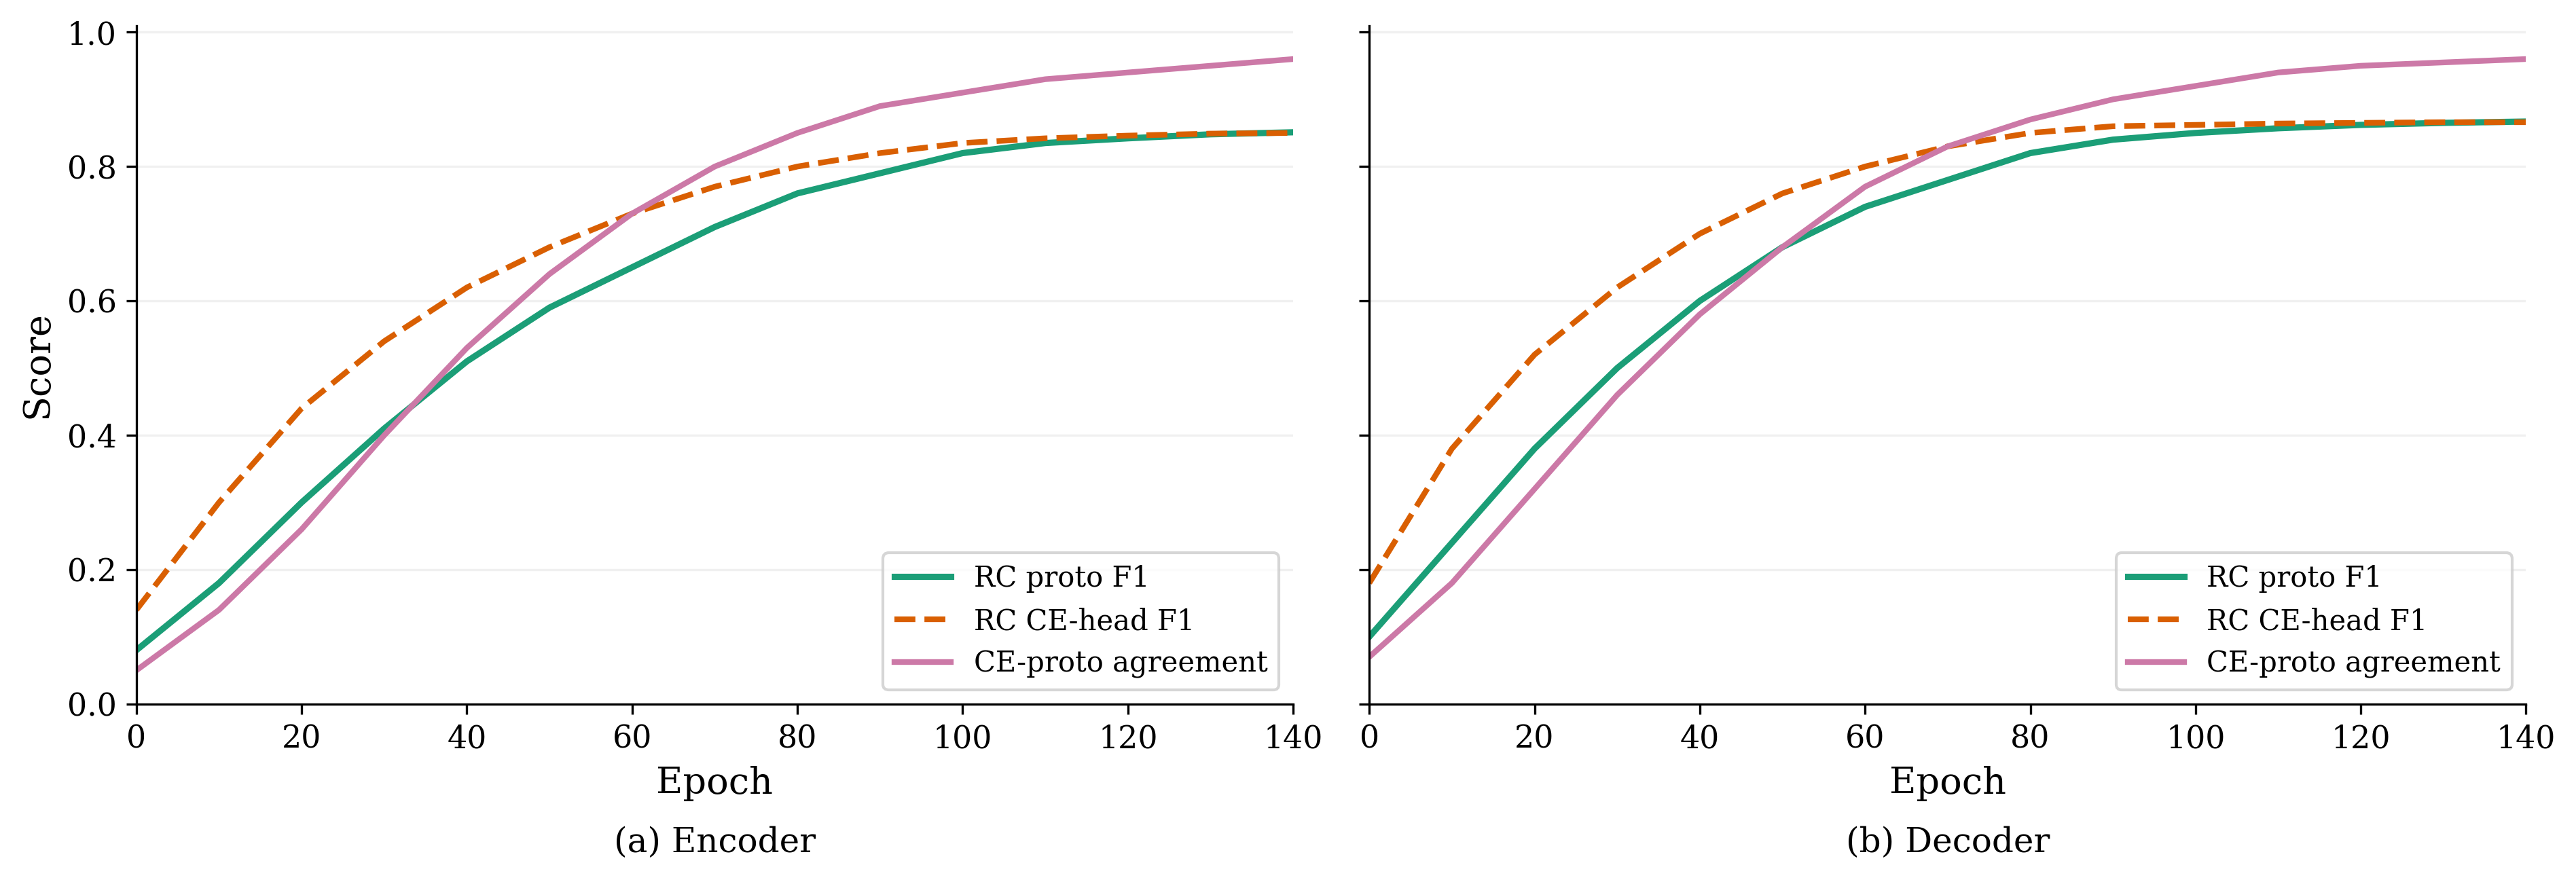
\includegraphics[width=0.9\linewidth]{fig_prototype_faithfulness.png}
\caption{Prototype-label agreement during training.}
\label{fig:defaultpp_prototype_faithfulness}
\end{figure}

\FloatBarrier

We test the explanation through group ablation. For each sample, we identify the two groups with the largest importance scores (Equation~\ref{eq:explanation}). Since the importance scores are normalized to sum to one and the distribution is typically concentrated on a few groups, in our experiment the top two groups were able to capture a substantial share of the total score. We zero out these two groups and compare the drop in the prototype margin (i.e., the gap between the predicted and nearest alternative prototype) with the drop obtained by zeroing two randomly chosen groups. Removing the most important groups reduces the gap more than removing random groups across all evaluated categories on both architectures (Figure~\ref{fig:rq3_group_ablation}). We conclude that the most important groups carry the diagnostic information that separates the predicted root cause from the nearest alternative. This ablation is a consistency check, not causal attribution. Ground-truth fault locations are not available for validation.

\begin{figure}[!htbp]
\centering
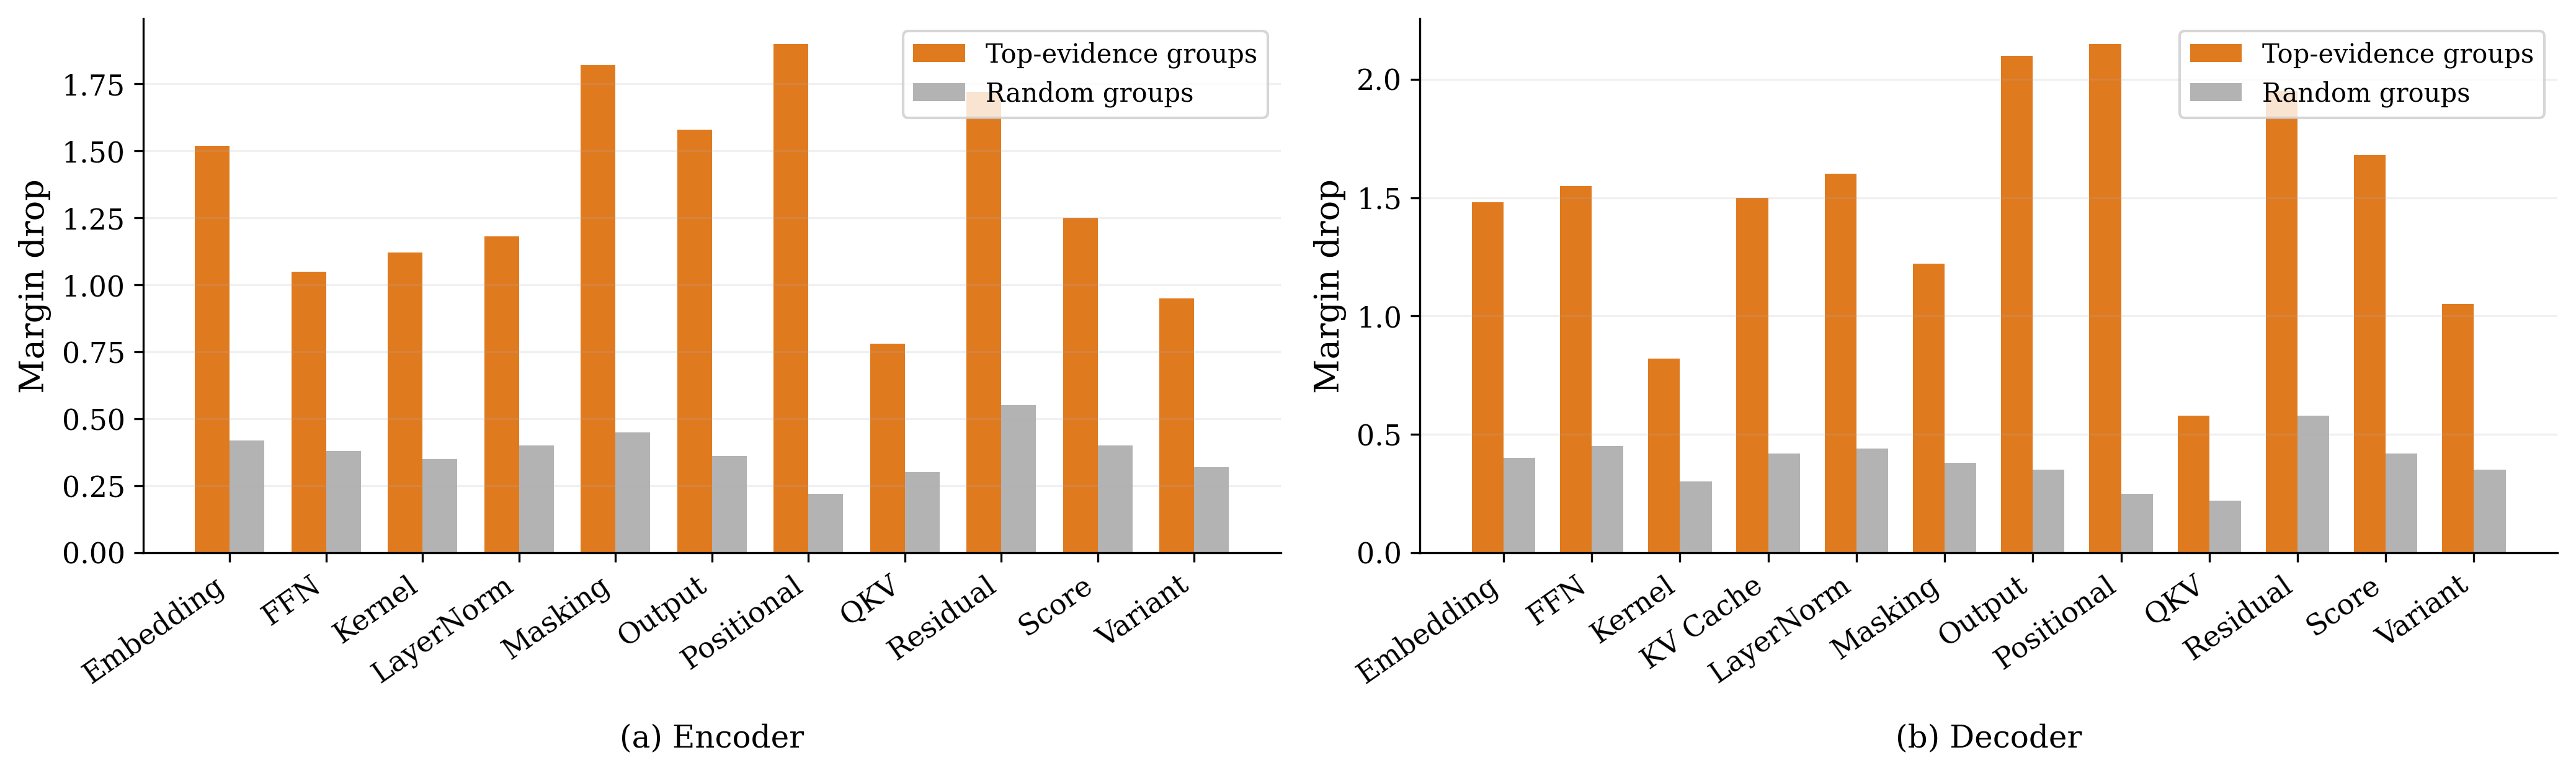
\includegraphics[width=0.9\linewidth]{fig_RQ3_group_ablation_faithfulness.png}
\caption{Group ablation analysis for the FPG-based explanation.}
\label{fig:rq3_group_ablation}
\end{figure}

% Old importance table and overlay/importance figures removed (superseded by group ablation analysis).

\FloatBarrier

\begin{rqsummary}
\textbf{Summary of RQ$\mathbf{_3}$:} When analyzing root causes of transformer faults, DEFault++'s Macro-F1 reaches 0.851 on encoders and 0.867 on decoders, with precision above 0.94. Level~2 errors constrain downstream root-cause accuracy. The group ablation confirms that the most important feature groups carry the diagnostic information that separates the predicted root cause from competing alternatives.
\end{rqsummary}

%==============================================================================
\section{Case Study: Evaluation of DEFault++}
\label{sec:defaultpp_casestudy}

We evaluated DEFault++ on real-world faults collected from open-source transformer repositories. We collected 11 confirmed faults (i.e.,~from bug-fix commits) from GitHub issue reports across jax-ml/jax, pytorch/pytorch, huggingface/transformers, huggingface/diffusers, google-ai-edge/ai-edge-torch, and lucidrains/nsa-pytorch. We reproduced each fault independently from the original issue report and instrumented it with the feature extraction technique described in Section~\ref{sec:defaultpp_features}. The faults span seven of the twelve Level~2 fault categories defined in the taxonomy (Masking, Positional, QKV, KV Cache, Score, Kernel, and Variant). Table~\ref{tab:realworld_eval} reports the results.

\begin{table*}[!htbp]
\centering
\caption[Real-world fault detection and diagnosis results.]{Real-world evaluation of DEFault++ on 11 transformer faults from six open-source repositories. Each fault was independently reproduced and diagnosed using extracted runtime features. Fault Category reports the Level~2 prediction. Discriminating Metric identifies the extraction metric that isolates the fault. \emph{(indirect)} marks cases where a related metric registers a downstream anomaly rather than the root cause directly. \emph{(none)} marks cases outside the current metric suite's coverage.}
\label{tab:realworld_eval}
\renewcommand{\arraystretch}{1.15}
\footnotesize
\begin{tabular}{@{}r l l l l p{3.6cm} r r r@{}}
\toprule
\textbf{\#} &
\textbf{Repository} &
\textbf{Issue} &
\textbf{Fault Category} &
\textbf{Component} &
\textbf{Discriminating Metric} &
\textbf{Faulty} &
\textbf{Fixed} &
\textbf{Flip Rate} \\
\midrule

1 & jax-ml/jax & \#23349
  & Masking
  & \texttt{dot\_product\_attention}
  & \texttt{attention\_mass\_pad\_mean}
  & 6.125 & 0.000 & 0.000$^{a}$ \\

2 & pytorch/pytorch & \#103082
  & Masking
  & \texttt{scaled\_dot\_product\_attn}
  & \texttt{attention\_mass\_future}
  & $>$0 & 0.000 & 1.000 \\

3 & huggingface/transformers & \#19045
  & Positional
  & \texttt{modeling\_bert.py}
  & \texttt{positional\_recv\_var} \emph{(indirect)}
  & $\downarrow$ & normal & 0.109 \\

4 & huggingface/transformers & \#17886
  & Positional
  & \texttt{modeling\_t5.py}
  & \texttt{head\_similarity\_mean} \emph{(indirect)}
  & $\uparrow$ & normal & 0.099 \\

5 & google-ai-edge/ai-edge-torch & \#6
  & QKV
  & Checkpoint loader
  & \texttt{pre\_softmax\_score\_var} \emph{(indirect)}
  & anom. & normal & 1.000$^\dagger$ \\

6 & lucidrains/nsa-pytorch & \#20
  & KV Cache
  & Transformer forward
  & \emph{(none)}
  & -- & -- & 0.820 \\

7 & huggingface/transformers & \#37574
  & KV Cache
  & \texttt{cache\_utils.py}
  & \emph{(none)}
  & -- & -- & 0.460 \\

8 & huggingface/transformers & \#36096
  & Score
  & \texttt{flex\_attention}
  & \emph{(none, extraction crash)}$^{*}$
  & crash & normal & 1.000$^\dagger$ \\

9 & pytorch/pytorch & \#116333
  & Kernel
  & Stride validator
  & \emph{(none)}
  & -- & -- & 1.000$^\dagger$ \\

10 & huggingface/transformers & \#35896
   & Variant
   & \texttt{modular\_qwen2.py}
   & \texttt{L\{idx\}\_attn\_entropy} \emph{(indirect)}
   & anom. & normal & 0.480 \\

11 & huggingface/diffusers & \#11903
   & QKV
   & \texttt{fuse\_qkv\_projections}
   & \texttt{qkv\_update\_ratio}
   & $\approx$0 & normal & 1.000 \\

\midrule
\multicolumn{4}{@{}l}{\textbf{Detection (Level~1)}} &
\multicolumn{5}{l}{8/11 faults detected\;\;(+1 via extraction crash$^{*}$;\;3 outside metric coverage)} \\
\multicolumn{4}{@{}l}{\textbf{Categorization (Level~2)}} &
\multicolumn{5}{l}{7/11 fault categories identified\;\;(3 direct, 4 indirect)} \\
\multicolumn{4}{@{}l}{\textbf{Root-Cause Diagnosis (Level~3)}} &
\multicolumn{5}{l}{4/11 root causes identified\;\;(cases 1, 2, 5, 11)} \\
\bottomrule
\end{tabular}

\vspace{2pt}
{\footnotesize
$^{a}$Fault signal present (padding attention mass = 6.125) but downstream predictions are not sensitive enough to flip on the evaluation set.\\
$^{*}$Case~8: the extraction process crashes on the malformed attention tensor. The crash is detectable as an error but is not a designed diagnostic metric.\\
$^\dagger$Cases where the faulty path produces an explicit failure (load error, invalid output, or backend rejection) before generating model output. Flip rate reflects the binary pass/fail transition after fix.\\
$\downarrow$ = decreased;\; $\uparrow$ = increased;\; anom.\ = anomalous distribution relative to healthy baseline.\\
Flip Rate = fraction of evaluation examples whose prediction differs between faulty and fixed paths (WikiText-103, PG19, or BoolQ).
}
\end{table*}

Detection performance is strongest for fault categories where a purpose-built metric directly matches the fault. We detect Cases~1 and~2 (Masking) through \texttt{attention\_mass\_pad\_mean} and \texttt{attention\_mass\_future}, which directly measure padding and causal mask behavior in the post-softmax attention distribution. We identify Case~11 (QKV) through the projection update ratio, which drops to near zero when LoRA adapts stale modules outside the active computation path. These three direct detections correspond to feature groups that received the highest importance scores in the FrankenFormer evaluation (Section~\ref{sec:defaultpp_rq3}), confirming that the same features that distinguish mutation-injected faults also identify naturally occurring faults in the same categories.

The four cases marked \emph{(indirect)} (Cases~3, 4, 5, and~10) show that a neighboring metric in the Fault Propagation Graph can register an anomaly when the fault propagates through connected components. We identify Cases~3 and~4 (Positional) through positional-sensitivity and head-similarity features that respond to downstream position-encoding anomalies. We detect Case~5 (QKV) through pre-softmax score variance, which shifts measurably when projection weights are missing or corrupted. In Case~10 (Variant), the fault misroutes sliding-window attention to the wrong layers, and the per-layer attention entropy metric registers the distributional shift even though we do not collect a dedicated window-routing metric. The propagation behavior is consistent with the forward sequential (M1) and cross-layer (M4) dependency mechanisms defined in Section~\ref{sec:defaultpp_fpg}. Adding targeted metrics for these fault classes would convert indirect detections into direct ones without requiring changes to the diagnostic model or the FPG structure.

Cases~6 and~7 involve KV Cache consistency faults that manifest during autoregressive generation rather than during fine-tuning. Our extraction technique collects cache-related metrics (cache hidden similarity and cache distribution divergence, as defined in Section~\ref{sec:defaultpp_features}), and these metrics are effective for cache faults that arise during the fine-tuning phase, as demonstrated on the FrankenFormer benchmark. However, the two KV Cache faults in this evaluation produce anomalies only at generation time, when cached key-value states from previous decoding steps interact with the current token. Extending the technique to instrument cached generation steps would bring these faults within coverage. Case~9 involves a kernel-dispatch fault that rejects a valid stride layout at the backend level. The kernel-dispatch fault operates below the model-behavior abstraction at which we collect features and would require system-level instrumentation to detect.

Case~8 presents a distinct failure mode. The faulty \texttt{flex\_attention} implementation returns a tensor with incorrect rank, which causes our extraction technique to crash rather than produce diagnostic features. The crash itself is detectable as an error, but it is not a designed diagnostic metric. We designed DEFault++ to diagnose silent faults that produce valid but incorrect output without raising exceptions. When a fault manifests as an explicit crash or exception, standard error-handling mechanisms are sufficient. Case~8 illustrates the boundary of our technique's target scope and confirms that DEFault++ addresses a complementary problem to runtime error detection.

We walk through Case~11 (Table~\ref{tab:realworld_eval}) as a detailed example. We introduced this fault as the motivating example in Section~\ref{sec:defaultpp_motivation}. The faulty program in Listing~\ref{lst:qkv_fusion_bug} fuses three projection layers into a single \texttt{to\_qkv} module but retains the original layers, which allows LoRA to attach to stale modules outside the active computation path. The fault produces no explicit error and the loss curve decreases normally, yet the fine-tuned model does not improve. We fine-tuned the model with the instrumentation from Section~\ref{sec:defaultpp_features} and ran DEFault++ on the collected trace. Figure~\ref{fig:defaultpp_case_qkv} shows the hierarchical predictions and per-group importance scores ($w_g$ from Equation~\ref{eq:explanation}) for a representative inference.

\begin{figure}[!htbp]
\centering
\begin{tikzpicture}[
    arrow/.style={-{Stealth[length=5pt]}, thick, black!50},
    barfill/.style={fill=rqblue, draw=rqblue!80},
    barfilllight/.style={fill=rqblue!25, draw=rqblue!40},
]

% === Layout constants ===
\def\labelwidth{3.6}   % width of level-label column
\def\contentstart{3.9}  % x where prediction text begins
\def\boxleft{0.0}
\def\boxright{13.0}
\def\boxmid{6.5}

% === Panel (a): Hierarchical diagnosis ===
\node[font=\small\bfseries, anchor=west] at (\boxleft, 0.3) {(a) Hierarchical diagnostic output};

% --- Level 1 ---
\draw[black!50, rounded corners=3pt] (\boxleft, -0.2) rectangle (\boxright, -1.4);
\fill[rqblue, rounded corners=2pt] (\boxleft+0.15, -0.5) rectangle (\boxleft+\labelwidth, -1.1);
\node[text=white, font=\footnotesize\bfseries] at (\boxleft+\labelwidth/2+0.075, -0.8) {Level 1: Detection};
\node[anchor=west, font=\small] at (\contentstart, -0.55) {\textbf{Faulty} \quad (confidence: 0.98)};
\node[anchor=west, font=\scriptsize, text=black!60] at (\contentstart, -1.05) {Normal training loss, abnormal projection-update behavior};

% Arrow
\draw[arrow] (\boxmid, -1.4) -- (\boxmid, -1.7);

% --- Level 2 ---
\draw[black!50, rounded corners=3pt] (\boxleft, -1.7) rectangle (\boxright, -2.9);
\fill[rqblue, rounded corners=2pt] (\boxleft+0.15, -2.0) rectangle (\boxleft+\labelwidth, -2.6);
\node[text=white, font=\footnotesize\bfseries] at (\boxleft+\labelwidth/2+0.075, -2.3) {Level 2: Categorization};
\node[anchor=west, font=\small] at (\contentstart, -2.05) {\textbf{QKV} fault category \quad (confidence: 0.91)};
\node[anchor=west, font=\scriptsize, text=black!60] at (\contentstart, -2.55) {Deviations in QKV alignment, projection update, attention entropy};

% Arrow
\draw[arrow] (\boxmid, -2.9) -- (\boxmid, -3.2);

% --- Level 3 ---
\draw[black!50, rounded corners=3pt] (\boxleft, -3.2) rectangle (\boxright, -4.4);
\fill[rqblue, rounded corners=2pt] (\boxleft+0.15, -3.5) rectangle (\boxleft+\labelwidth, -4.1);
\node[text=white, font=\footnotesize\bfseries] at (\boxleft+\labelwidth/2+0.075, -3.8) {Level 3: Root cause};
\node[anchor=west, font=\small] at (\contentstart, -3.55) {\textbf{Stale-parameter fault} \quad (confidence: 0.88)};
\node[anchor=west, font=\scriptsize, text=black!60] at (\contentstart, -4.05) {Near-zero update ratio for \texttt{q\_proj}/\texttt{v\_proj}, fused path active};

% === Panel (b): Salience bar chart ===
\node[font=\small\bfseries, anchor=west] at (\boxleft, -5.2) {(b) Feature-group importance ($w_g$)};

\def\barlabelwidth{2.8}  % width reserved for bar labels
\def\barstart{3.0}
\def\barscale{7.0}
\def\barheight{0.32}
\def\bartextoffset{0.15}

% QKV alignment: 45%
\node[anchor=east, font=\scriptsize] at (\barstart - 0.15, -5.9) {QKV alignment};
\fill[barfill] (\barstart, -5.9-\barheight/2) rectangle (\barstart+0.45*\barscale, -5.9+\barheight/2);
\node[anchor=west, font=\scriptsize\bfseries] at (\barstart+0.45*\barscale+\bartextoffset, -5.9) {45\%};

% Training dynamics (update ratios): 28%
\node[anchor=east, font=\scriptsize] at (\barstart - 0.15, -6.4) {Training dynamics};
\fill[barfill] (\barstart, -6.4-\barheight/2) rectangle (\barstart+0.28*\barscale, -6.4+\barheight/2);
\node[anchor=west, font=\scriptsize\bfseries] at (\barstart+0.28*\barscale+\bartextoffset, -6.4) {28\%};

% Attention: 12%
\node[anchor=east, font=\scriptsize] at (\barstart - 0.15, -6.9) {Attention};
\fill[barfilllight] (\barstart, -6.9-\barheight/2) rectangle (\barstart+0.12*\barscale, -6.9+\barheight/2);
\node[anchor=west, font=\scriptsize] at (\barstart+0.12*\barscale+\bartextoffset, -6.9) {12\%};

% Score: 7%
\node[anchor=east, font=\scriptsize] at (\barstart - 0.15, -7.4) {Score};
\fill[barfilllight] (\barstart, -7.4-\barheight/2) rectangle (\barstart+0.07*\barscale, -7.4+\barheight/2);
\node[anchor=west, font=\scriptsize] at (\barstart+0.07*\barscale+\bartextoffset, -7.4) {7\%};

% Other groups: 8%
\node[anchor=east, font=\scriptsize] at (\barstart - 0.15, -7.9) {Other groups};
\fill[barfilllight] (\barstart, -7.9-\barheight/2) rectangle (\barstart+0.08*\barscale, -7.9+\barheight/2);
\node[anchor=west, font=\scriptsize] at (\barstart+0.08*\barscale+\bartextoffset, -7.9) {8\%};

% Annotation brace for QKV + Training dynamics
\draw[decorate, decoration={brace, amplitude=5pt, mirror}, thick, rqblue]
    (\barstart+0.45*\barscale+0.8, -5.9+\barheight/2+0.05)
    -- (\barstart+0.45*\barscale+0.8, -6.4-\barheight/2-0.05)
    node[midway, right=6pt, font=\scriptsize, text=rqblue, align=left] {73\% in QKV alignment\\and training dynamics};

\end{tikzpicture}
\caption{DEFault++ diagnostic output for the stale QKV fusion fault (Listing~\ref{lst:qkv_fusion_bug}). Panel~(a) shows hierarchical predictions with confidence scores. Panel~(b) shows normalized feature-group importance scores for a representative inference.}
\label{fig:defaultpp_case_qkv}
\end{figure}

\paragraph{Level 1: Fault detection.}
DEFault++ applies binary detection to the trace and marks the instance as faulty (Figure~\ref{fig:defaultpp_case_qkv}). The detection is driven by projection-update features, not by global training failure. The loss decreased normally throughout training, and no aggregate optimization metric registered an anomaly. However, the internal projection-update measurements deviated from the behavior of clean configurations in the training data. The Fault Propagation Graph propagated this deviation across connected feature groups before classification.

\paragraph{Level 2: Fault categorization.}
DEFault++ classifies the instance into the \textit{QKV} fault category. We observe the primary evidence in three feature groups. First, the projection update ratios for \texttt{q\_proj} and \texttt{v\_proj} remain near zero, indicating no effective update. Second, the pairwise Q--K, Q--V, and K--V alignment features deviate from the pattern of actively fine-tuned projections. Third, attention entropy and pre-softmax scores shift toward patterns associated with disturbed projection coherence, not masking, positional, or residual-stream faults.

\paragraph{Level 3: Root cause diagnosis.}
DEFault++ predicts a \textit{weight-update / stale-parameter fault} by comparing the trace with per-root-cause prototypes in the embedding space. QKV alignment and training dynamics provide most of the evidence, together accounting for 73\% of the normalized importance (Figure~\ref{fig:defaultpp_case_qkv}b). Attention and score features provide secondary support. The observed pattern is consistent with a stale-parameter fault. The model trains, but the adapted parameters are disconnected from the computation that produces the output. In Listing~\ref{lst:qkv_fusion_bug}, the \texttt{forward} method consumes \texttt{to\_qkv}, while the \texttt{q\_proj} and \texttt{v\_proj} attributes remain addressable to downstream adapters. The explanation highlights the QKV alignment and gradient feature groups, which correspond to the projection code path where the fault originates. While individual feature values such as near-zero update ratios are observable in isolation, identifying which combination of feature-group deviations maps to which root cause across 45 possible root causes requires the learned classifier. None of the four baseline techniques (e.g.,~AutoTrainer, DeepDiagnosis, DeepFD, DEFault) detected this fault, as the training process remained within the boundaries of their monitored criteria and the fault produced no numerical errors.

%==============================================================================
\section{Developer Study}
\label{sec:defaultpp_devstudy}

We evaluated the usefulness and actionability of DEFault++ diagnostic output in a developer study with 21 practitioners~\cite{amershi2019software}. Participants reviewed four debugging scenarios derived from reproduced real-world transformer faults and selected repair actions under two conditions: a baseline condition with scenario materials only, and a DEFault++-assisted condition with the same materials plus the diagnostic output. The study measured whether the diagnostic output helped participants choose correct repair actions, and whether participants perceived the output as clear, useful, and actionable.

\subsection{Study Design}
\label{sec:defaultpp_devstudy_design}

We used a within-subjects, counterbalanced design with two conditions~\cite{wohlin2012experimentation}. In the \emph{baseline} condition, participants received a scenario description, observed behavior, and logs with metrics. In the \emph{DEFault++-assisted} condition, participants received the same materials plus four fields from the DEFault++ diagnostic output: predicted fault status, predicted fault category, predicted root cause, and predicted fault component. We created two survey forms (A and~B) to counterbalance condition assignment across scenarios. Form~A assigned Scenarios~1 and~3 to the baseline condition and Scenarios~2 and~4 to the assisted condition. Form~B reversed this assignment. Each participant completed all four scenarios, two per condition. This scenario-based evaluation follows the approach used in prior developer studies of DL debugging tools~\cite{umlaut,kunit}.

We derived the four scenarios from reproduced real-world GitHub issues, each representing a distinct transformer fault category (Table~\ref{tab:devstudy_scenarios}). Each scenario included four repair options: one correct option matching the actual fix applied in the source issue, two incorrect options targeting related components, and one unrelated option targeting training hyperparameters. The correct repair required one inferential step beyond the shown diagnosis. A DEFault++ report identifying an ``attention masking fault'' does not by itself name the specific code-level fix. The participant must translate the diagnosis into an engineering action, which is the outcome we measured.

\begin{table}[!htbp]
\centering
\caption{Developer study scenarios with source issues, fault categories, and counterbalanced condition assignments.}
\label{tab:devstudy_scenarios}
\small
\begin{tabular}{@{}r l l l l l@{}}
\toprule
\textbf{\#} & \textbf{Scenario} & \textbf{Source Issue} & \textbf{Fault Category} & \textbf{Form~A} & \textbf{Form~B} \\
\midrule
1 & Cached Decoding Visibility  & pytorch \#103082       & Masking     & Baseline  & Assisted \\
2 & Position Scoring Drift      & transformers \#19045   & Positional  & Assisted  & Baseline \\
3 & Incremental State Mismatch  & nsa-pytorch \#20       & KV Cache    & Baseline  & Assisted \\
4 & Wrong Layer Assignment      & transformers \#35896   & Variant     & Assisted  & Baseline \\
\bottomrule
\end{tabular}
\end{table}

We measured three primary outcomes per scenario: repair action correctness (binary, scored against the ground-truth fix from the source issue), self-reported confidence (5-point ordinal scale from ``not confident at all'' to ``very confident''), and self-reported time (categorical bins from ``less than a minute'' to ``more than 10~minutes''). After completing all four scenarios, participants rated three perception statements on a 5-point Likert agreement scale and answered two forced-choice preference questions comparing the baseline and assisted conditions.

% === Participants ===

\subsection{Participants}
\label{sec:defaultpp_devstudy_participants}

We recruited participants through graduate student mailing lists, academic networks, and direct outreach. The Dalhousie University Research Ethics Board reviewed and approved this study. Eligibility required experience with transformer architectures in at least one of training, fine-tuning, inference, debugging, or evaluation~\cite{umlaut,kunit}. We excluded anyone enrolled in a course taught by the lead researcher or directly supervised by the research team. Twenty-one practitioners completed the study (12 via Form~A, 9 via Form~B). Participation was anonymous, voluntary, and uncompensated. Estimated completion time was 10 to 15~minutes. We hosted the study on Microsoft Forms.

\begin{table}[!htbp]
\centering
\caption{Developer study participant demographics (N\,=\,21).}
\label{tab:devstudy_demographics}
\small
\begin{tabular}{@{}l l r r@{}}
\toprule
\textbf{Characteristic} & \textbf{Value} & \textbf{N} & \textbf{\%} \\
\midrule
ML/DL experience & Less than 1 year & 1 & 5 \\
                 & 1--2 years       & 6 & 29 \\
                 & 3--5 years       & 10 & 48 \\
                 & More than 5 years & 4 & 19 \\
\addlinespace
Prior transformer debugging & Yes & 15 & 71 \\
                            & No  & 6  & 29 \\
\addlinespace
Role (multi-select) & Research assistant      & 10 & -- \\
                    & Graduate student        & 11 & -- \\
                    & Industry practitioner   & 9  & -- \\
\bottomrule
\end{tabular}
\end{table}

Ten participants (48\%) had 3 to 5~years of ML/DL experience, and 15~(71\%) had prior experience debugging transformer models. Participants spanned academic and industry roles (Table~\ref{tab:devstudy_demographics}).

% === Results ===

\subsection{Results}
\label{sec:defaultpp_devstudy_results}

\paragraph{Repair accuracy.}
Across all 21 participants and four scenarios, participants selected the correct repair action in 24 of 42 baseline responses (57.1\%) and 35 of 42 assisted responses (83.3\%), an improvement of +26.2\% under the DEFault++-assisted condition. Table~\ref{tab:devstudy_results} reports the per-scenario breakdown. The largest accuracy gain appeared in Scenario~2 (Positional fault, +38.9\%), which had the subtlest symptom profile (flip rate 0.109, output delta 0.025) and the lowest baseline accuracy (44.4\%). Scenario~1 reached 100\% accuracy under the assisted condition. Under the baseline condition, 16 of 18 incorrect responses selected a related but incorrect option, and only 2 selected the unrelated hyperparameter option. Under the assisted condition, no participant selected the unrelated option. Figure~\ref{fig:devstudy_results} shows the per-scenario accuracy comparison and perception ratings.

\begin{figure}[!htbp]
\centering
\begin{subfigure}[t]{0.52\textwidth}
\centering
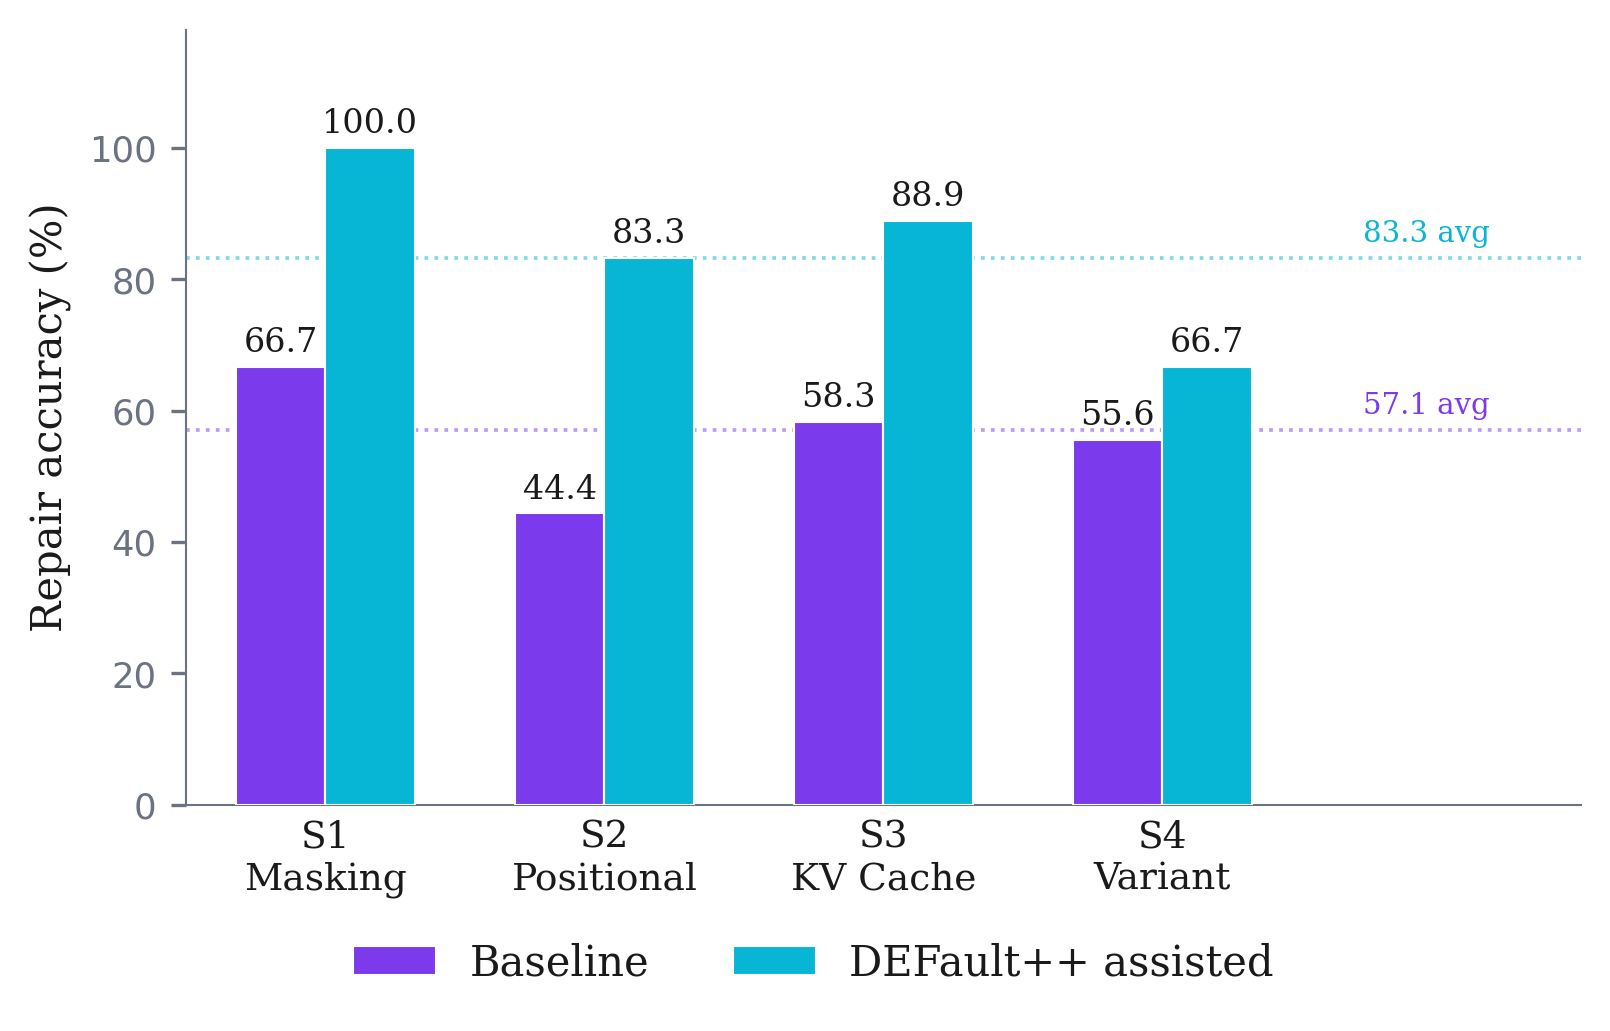
\includegraphics[width=\linewidth]{fig_devstudy_accuracy.png}
\caption{Repair accuracy by scenario and condition. Dotted lines indicate aggregate accuracy (57.1\% baseline, 83.3\% assisted).}
\label{fig:devstudy_accuracy}
\end{subfigure}%
\hfill
\begin{subfigure}[t]{0.46\textwidth}
\centering
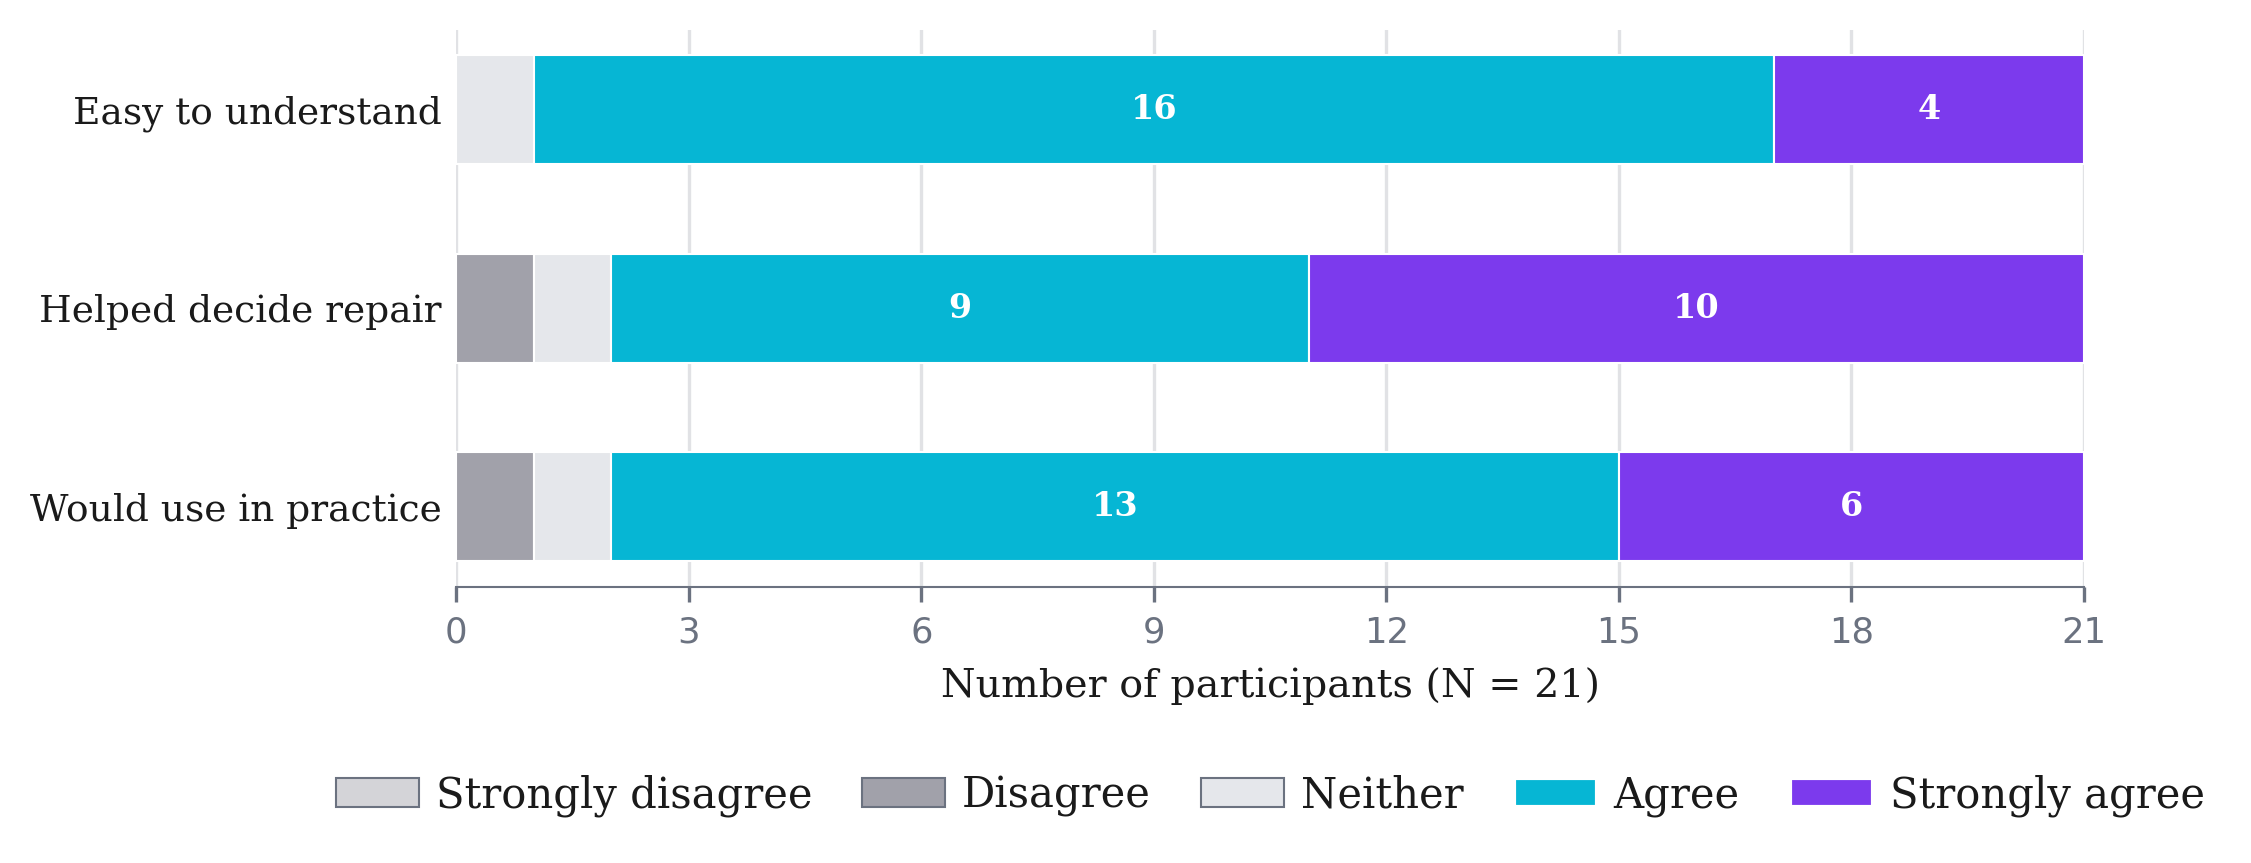
\includegraphics[width=\linewidth]{fig_devstudy_likert.png}
\caption{Likert agreement ratings for three perception statements (N\,=\,21). Across all items, 92\% agreed or strongly agreed.}
\label{fig:devstudy_likert}
\end{subfigure}
\caption{Developer study results. (a)~Per-scenario repair accuracy under baseline and DEFault++-assisted conditions. (b)~Participant perception of DEFault++ diagnostic output.}
\label{fig:devstudy_results}
\end{figure}

\begin{table}[!htbp]
\centering
\caption{Repair accuracy, confidence, and time by scenario and condition.}
\label{tab:devstudy_results}
\small
\begin{tabular}{@{}l l r l r r r@{}}
\toprule
\textbf{Scenario} & \textbf{Condition} & \textbf{N} & \textbf{Correct} & \textbf{Acc.} & \textbf{Conf.} & \textbf{Time} \\
\midrule
S1 (Masking)     & Baseline  & 12 & 8/12  & 66.7\% & 3.75 & 3.3\,m \\
S1 (Masking)     & Assisted  &  9 & 9/9   & 100.0\% & 4.11 & 2.3\,m \\
\addlinespace
S2 (Positional)  & Baseline  &  9 & 4/9   & 44.4\% & 2.78 & 2.6\,m \\
S2 (Positional)  & Assisted  & 12 & 10/12 & 83.3\% & 3.75 & 4.1\,m \\
\addlinespace
S3 (KV Cache)    & Baseline  & 12 & 7/12  & 58.3\% & 3.50 & 3.2\,m \\
S3 (KV Cache)    & Assisted  &  9 & 8/9   & 88.9\% & 4.11 & 1.8\,m \\
\addlinespace
S4 (Variant)     & Baseline  &  9 & 5/9   & 55.6\% & 3.33 & 2.7\,m \\
S4 (Variant)     & Assisted  & 12 & 8/12  & 66.7\% & 4.08 & 3.1\,m \\
\midrule
Total            & Baseline  & 42 & 24/42 & 57.1\% & 3.38 & 3.0\,m \\
Total            & Assisted  & 42 & 35/42 & 83.3\% & 4.00 & 2.9\,m \\
\bottomrule
\end{tabular}
\end{table}

\paragraph{Confidence.}
Participants reported higher confidence under the assisted condition (M\,=\,4.00, SD\,=\,0.83) than the baseline condition (M\,=\,3.38, SD\,=\,1.08). Confidence was calibrated under both conditions. On correct responses, mean confidence was 3.75 (baseline) and 4.11 (assisted). On incorrect responses, mean confidence was 2.89 (baseline) and 3.43 (assisted). The gap between correct and incorrect responses persisted under both conditions, which indicates that DEFault++ raised confidence without decoupling it from accuracy. The largest confidence gain appeared in Scenario~2 (2.78 to 3.75), the scenario with the subtlest symptoms and the lowest baseline accuracy.

\paragraph{Self-reported time.}
Self-reported time was comparable between conditions, with the assisted condition marginally faster on average than the baseline condition. Scenario~2 was the only scenario where participants reported spending more time under the assisted condition than under the baseline. This pattern is consistent with participants reading the DEFault++ output more carefully on the hardest scenario before committing to a repair action.

\paragraph{Perception of DEFault++ output.}
Across all 21 participants, 20~(95\%) agreed or strongly agreed that the DEFault++ output was easy to understand (M\,=\,4.14, SD\,=\,0.48). 19~(90\%) agreed or strongly agreed that the output helped them decide what repair to try first (M\,=\,4.29, SD\,=\,0.96). The same proportion agreed or strongly agreed that they would use a tool like DEFault++ in practice (M\,=\,4.10, SD\,=\,0.89). On the preference questions, 15~participants (71\%) reported that the assisted condition better supported their debugging decision, and 16~(76\%) perceived it as faster. One participant (5\%) preferred the baseline condition on each question. Figure~\ref{fig:devstudy_likert} shows the response distribution across all three Likert items.

\paragraph{Within-subjects comparison.}
Each participant served as their own control with two baseline and two assisted scenarios. Per-participant mean accuracy was 0.571 (SD\,=\,0.427) under the baseline condition and 0.833 (SD\,=\,0.289) under the assisted condition. Of the 21~participants, 7 improved under the assisted condition, 14 showed no change, and none declined. No participant performed worse with DEFault++ assistance than without it.

% === Discussion ===

\subsection{Discussion}
\label{sec:defaultpp_devstudy_discussion}

DEFault++ assistance improved repair accuracy from 57.1\% to 83.3\% across the four evaluated scenarios. The improvement was largest where the fault was hardest to localize from symptoms alone. Scenario~2 (Positional fault) had the subtlest behavioral signal and showed the largest accuracy gain (+38.9\%) and the largest confidence gain (+0.97). Scenario~4 (Variant fault) had the most transparent symptom-to-repair mapping and showed the smallest accuracy gain (+11.1\%). This pattern suggests that the value of DEFault++ diagnostic output concentrates on faults where the symptom-to-cause mapping is ambiguous rather than on faults where the correct action is already apparent from the scenario description.

Under the baseline condition, errors were overwhelmingly related but incorrect options (16 of 18, or 89\%), not random or unrelated choices. Participants engaged with the scenario content but lacked sufficient diagnostic information to distinguish between related components (e.g.,~masking vs.\ position encoding in Scenario~1). Under the assisted condition, the DEFault++ output resolved this ambiguity for most participants. The zero-decline result (no participant performed worse with DEFault++ than without it) indicates that the diagnostic output did not mislead participants, even in the seven cases where the assisted response was still incorrect.

The perception data reinforces the accuracy findings. Across all three Likert items, 92\% of participants agreed or strongly agreed, and 71\% preferred the assisted condition for decision support. These perception ratings are consistent with findings reported in related developer studies. Schoop~et~al.~\cite{umlaut} found that participants using UMLAUT rated the tool positively for helping them find (M\,=\,4.3) and fix (M\,=\,4.0) bugs, and Manke~et~al.~\cite{kunit} found that 34 of 36 participants rated mocks as helpful for independent component testing.

This study evaluates actionability under correct diagnoses on four decoder/generation-path scenarios. The study does not test trust calibration when DEFault++ produces an incorrect diagnosis, and the four scenarios do not cover the full taxonomy evaluated in the preceding sections. A larger study with incorrect diagnoses and broader fault coverage would strengthen the external validity of these findings.

\section{Limitations and Future Directions}
\label{sec:defaultpp_limitations}

Our proposed Fault Propagation Graph (FPG) assumes that faults always propagate along the deterministic edges derived from the forward and backward pass. In practice, successive matrix multiplications, normalization layers, and nonlinear activations can reduce or eliminate the effect of a perturbation before it reaches a downstream component. The current FPG does not model this reduction. Future work can target a fault-injection study to test whether downstream feature groups change as the FPG predicts. 

The FPG also abstracts component-level computation under a standard transformer block structure and does not model architecture-specific parameter-tying shortcuts (e.g., tied input-embedding, output-head weights in GPT-2-style decoders) (see Table~\ref{tab:fpg_derivation}). Architectures that differ from the standard transformer block layout may introduce propagation paths that the current graph does not represent. Future work can extend the graph with such architecture-specific edges and with relation-typed message passing that distinguishes the three mechanism classes. 

Our benchmark covers seven transformer models and nine tasks with single-fault configurations. This scope does not include compound faults (i.e., two or more faults within the same instance) and also does not cover larger-scale architectures (e.g., mixture-of-experts, multimodal cross-attention models). Future work can extend the evaluation along both dimensions. 


%==============================================================================
\section{Threats to Validity}
\label{sec:defaultpp_threats}

Threats to \emph{internal validity}~\cite{wohlin2012experimentation} relate to experimental errors. The main threat is information leakage among configurations sharing the same model, dataset, and seed. We mitigate this through nested grouped cross-validation, fitting all preprocessing and hyperparameter selection exclusively on the inner-training fold, and applying the same outer fold assignments across all compared methods. A second threat is the joint training objective, where the shared encoder means that changes in one loss can affect the representation available to the others. In particular, the separation loss targets Level~3 root-cause discrimination and may steer the shared representation in ways that do not benefit Level~1 detection or Level~2 categorization. We examine this interaction through the ablation in RQ$\mathbf{_2}$, which independently removes each component and measures the performance change at every level.

Threats to \emph{construct validity}~\cite{wohlin2012experimentation} relate to whether the benchmark represents the intended diagnosis problem. The benchmark is produced by mutation operators rather than by naturally occurring faults~\cite{attention_taxonomy,frankenformer}. We mitigate this threat by deriving the mutation operators from the attention fault taxonomy (Chapter~\ref{chapter_attention}), which we constructed from 555 real-world faults collected from open-source repositories. Because the mutation operators come from observed faults in real-world repositories, the injected faults reflect real failure mechanisms. Five-seed averaging may obscure transient training behaviors. We mitigate this by recording per-seed measurements before averaging and by reporting within-epoch variance as a feature (Section~\ref{sec:defaultpp_features}). Class imbalance is another construct-validity threat. We addressed this through Macro-F1 reporting and inverse-frequency class weighting~\cite{buda2018systematic}. We test the explanation through group ablation (RQ$\mathbf{_3}$), which checks internal consistency between the importance scores and the model's decision, and through a code-level check in the real-world evaluation (Section~\ref{sec:defaultpp_casestudy}). These tests are internal checks, not independent external validation. The developer study (Section~\ref{sec:defaultpp_devstudy}) provides a preliminary evaluation of whether the diagnostic output is actionable in practice.

Threats to \emph{external validity}~\cite{wohlin2012experimentation} relate to generalizability. The dataset covers seven transformer models and nine tasks~\cite{frankenformer}. We mitigate the risk of model-specific overfitting by using nested grouped cross-validation where each fold groups all seeds and tasks for a given model together, ensuring the classifier generalizes across models. We report per-fold standard deviations and use the same folds across compared methods to make variation visible. Existing baselines do not expose a label space compatible with our fault categories, so we restrict direct comparison to Level~1 detection and report baseline coverage separately (Table~\ref{tab:baseline_coverage}).

The developer study (Section~\ref{sec:defaultpp_devstudy}) introduces additional validity considerations. The sample size is modest (N\,=\,21), though the within-subjects paired design partially mitigates this limitation. The study uses a vignette-based design where participants read scenario descriptions rather than interact with DEFault++ in a live debugging environment. This design isolates the diagnostic signal from tool usability confounds but does not capture real-world debugging workflows. Self-reported time is a perceived-effort proxy rather than an objective performance measure. The four scenarios cover only decoder/generation-path faults and do not span the full taxonomy evaluated in the preceding sections. The assisted condition always shows a technically correct diagnosis. The study therefore evaluates actionability conditional on correct output rather than trust calibration under model error.


%==============================================================================
\section{Related Work}
\label{sec:defaultpp_related}

\textbf{Debugging DNN Programs.}
Rule-based debuggers such as AutoTrainer~\cite{autotrainer}, DeepDiagnosis~\cite{deepdiagnosis}, and UMLAUT~\cite{umlaut} reason over generic training symptoms. Learning-based approaches such as DeepFD~\cite{deepfd} and our prior work DEFault~\cite{default} move from fixed rules to classifiers over runtime traces. DeepFD and DEFault are most closely aligned with DEFault++, but they still predict DNN-level fault types rather than transformer component categories and within-category root causes, making them less applicable. A label space built for loss functions, activations, or optimizers does not directly express QKV, masking, positional, residual, or KV-cache faults. DeepLocalize~\cite{deeplocalize} traces numerical failures back to layers from runtime values, while static analyzers such as NeuraLint~\cite{NeuraLint}, NerdBug~\cite{nerdbug}, DEBAR~\cite{debar}, and BugLab~\cite{buglab} inspect structure without training execution. FL4Deep~\cite{fl4deep} combines static code features with dynamic features through a knowledge graph. DEFault++ instead targets runs that remain structurally valid and numerically stable but leave component-specific behavioral traces during training. Static analyzers could serve as complementary baselines for faults that manifest as structural data-flow mismatches (e.g., the QKV fusion case in Section~\ref{sec:defaultpp_casestudy}), but their label space does not align with the component-level fault categories defined by the attention fault taxonomy, and they do not produce diagnoses from runtime traces.

\textbf{Transformer-Specific Analysis.}
Some prior work is transformer-specific but addresses a different fault model. Adversarial evaluation, behavioral testing, and attention analysis approaches study robustness and behavior under perturbation~\cite{jones2020adversarial,ribeiro2020checklist,clark2019does,voita2019analyzing}. Systems-level methods such as ATTNChecker~\cite{liang2025attnchecker}, FT-Transformer~\cite{fttransformer}, AtPatch~\cite{atpatch2026}, and Bug Attention Probe~\cite{bap2025} focus on transient numerical faults, tolerance mechanisms, or attention-map anomalies. The cited studies show that transformers require dedicated analysis, but they do not address supervised diagnosis of persistent implementation faults across component categories and root causes. LLM-based debugging assistants such as SoapFL~\cite{soapfl2025}, LLM4FL~\cite{llm4fl2024}, ChatDBG~\cite{chatdbg2025}, and BugReAct~\cite{bugreact2026} assist source-level debugging in general software rather than learning a transformer fault classifier from instrumented traces.

\textbf{Mutation Testing.}
Supervised fault diagnosis depends on labeled faulty runs, and mutation testing has been the main way to construct such data. DeepMutation~\cite{deepmutation}, DeepMutation++~\cite{deepmutation++}, and DeepCrime~\cite{deepcrime} expanded mutation testing for DNNs, but their operators target generic DNN components rather than attention-specific mechanisms. FrankenFormer~\cite{frankenformer} injects transformer-specific faults and records internal measurements relevant to attention behavior. DEFault++ uses that benchmark for its training and evaluation, and therefore provides the data needed to evaluate DEFault++.

\textbf{Explainability.}
Most explanation methods used in software engineering and prior fault diagnosis are post-hoc. Representative examples include SHAP, DiCE, and Anchors~\cite{lundberg2017unified,mothilal2020dice,ribeiro2018anchors}, which return feature attributions, counterfactuals, or rules after the classifier has already made its decision. DEFault (Chapter~\ref{chapter_default}) used this style of explanation in a cascaded way for diagnosis. DEFault++ uses a different strategy. The Level~3 diagnosis is defined through prototype comparison in a grouped embedding space, and the reported explanation decomposes the gap between the predicted prototype and the nearest alternative across feature groups. We adapted this design choice from the existing works on prototype networks~\cite{snell2017prototypical} and concept-bottleneck ideas~\cite{koh2020concept}, but here the groups correspond to transformer subsystems rather than to semantic concepts.


%==============================================================================
\section{Conclusion}
\label{sec:defaultpp_summary}

This chapter summarizes DEFault++, a transformer-specific extension of DEFault. DEFault showed that hierarchical diagnosis can support fault detection and categorization for FFNNs, CNNs, and RNNs using DNN-level static and dynamic features. DEFault++ extends that framework to transformer architectures and highlights which feature groups provide the main evidence for each diagnosis. DEFault++ organizes the diagnosis around a Fault Propagation Graph, which encodes how faults propagate between transformer components. On the FrankenFormer benchmark, DEFault++ achieves AUROC above 0.96 for detection, Macro-F1 above 0.85 for categorization, and hierarchical root-cause Macro-F1 above 0.85 on both encoder and decoder architectures. These results show that transformer traces are informative enough to support automated fault detection, categorization, and hierarchical root-cause diagnosis. In a developer study with 21 practitioners, DEFault++ diagnostic output improved repair action accuracy from 57.1\% to 83.3\%, and 90\% of participants agreed that they would use the tool in practice.

